\documentclass[12pt,a4paper]{amsart}
\usepackage[utf8]{inputenc}
\usepackage[T1]{fontenc}
\usepackage{amsmath,amsfonts,amssymb}
\usepackage{tikz}
\usepackage{algorithm,algcompatible,amssymb,amsmath}
\renewcommand{\COMMENT}[2][.5\linewidth]{%
  \leavevmode\hfill\makebox[#1][l]{//~#2}}
\algnewcommand\algorithmicto{\textbf{to}}
\algnewcommand\TO{\textbf{ to }}
\algnewcommand\AND{\textbf{ and }}
\algnewcommand\RETURN{\State \textbf{return} }
\usepackage{float}
\usepackage{listings}
\usepackage[table]{xcolor}
\usepackage{caption}
\usepackage{geometry}
\usepackage{fancyhdr}
\usepackage{enumitem}
\usepackage{booktabs}
\usepackage{multirow}
\usepackage[hidelinks,bookmarksnumbered,bookmarksopen,colorlinks=true,linkcolor=red,urlcolor=red,citecolor=red]{hyperref}

\usepackage{xeCJK}
\usepackage{docmute}  % 关键宏包:自动忽略被包含文件的前言部分
\setCJKmainfont{LXGW WenKai}
% Define custom colors
\definecolor{lightblue}{RGB}{173,216,230}
\definecolor{lightgreen}{RGB}{144,238,144}
\definecolor{lightyellow}{RGB}{255,255,224}
\definecolor{lightgray}{RGB}{211,211,211}
\geometry{left=2.5cm,right=2.5cm,top=2.5cm,bottom=2.5cm}
\renewcommand{\arraystretch}{1.5}

% 代码高亮设置
\lstset{
    language=C++,
    basicstyle=\ttfamily\small,
    keywordstyle=\color{blue}\bfseries,
    commentstyle=\color{green!60!black},
    stringstyle=\color{red},
    numbers=left,
    numberstyle=\tiny\color{gray},
    stepnumber=1,
    numbersep=10pt,
    backgroundcolor=\color{gray!10},
    frame=single,
    tabsize=4,
    captionpos=b,
    breaklines=true,
    breakatwhitespace=false,
    showspaces=false,
    showstringspaces=false,
    showtabs=false
}

% 定理环境
\newtheorem{definition}{定义}[section]
\newtheorem{theorem}{定理}[section]
\newtheorem{example}{例题}[section]
\newtheorem{property}{性质}[section]

% TikZ库
\usetikzlibrary{positioning,arrows,automata,calc,shapes,patterns}

\title{\textbf{数据结构 - 合并版复习资料}}
\author{复习资料}
\date{\today. \textit{Author}: 乐绎华}

\begin{document}

\maketitle
\tableofcontents
\newpage

% 使用docmute宏包后,可以直接包含完整的.tex文件
% docmute会自动忽略被包含文件的\documentclass、\begin{document}、\end{document}等
\part{线性表}
\documentclass[12pt,a4paper]{amsart}
\usepackage[utf8]{inputenc}
\usepackage[T1]{fontenc}
\usepackage{amsmath,amsfonts,amssymb}
\usepackage{tikz}
\usepackage{algorithm}
\usepackage{algorithmic}
\usepackage{float}
\usepackage{listings}
\usepackage{xcolor}
\usepackage{geometry}
\usepackage{fancyhdr}
\usepackage{enumitem}
\usepackage{booktabs}
\usepackage{multirow}
\usepackage[hidelinks,bookmarksnumbered,bookmarksopen]{hyperref}
\usepackage{xeCJK}
\setCJKmainfont{LXGW WenKai}

\geometry{left=2.5cm,right=2.5cm,top=2.5cm,bottom=2.5cm}

% 代码高亮设置
\lstset{
    language=C++,
    basicstyle=\ttfamily\small,
    keywordstyle=\color{blue}\bfseries,
    commentstyle=\color{green!60!black},
    stringstyle=\color{red},
    numbers=left,
    numberstyle=\tiny\color{gray},
    stepnumber=1,
    numbersep=10pt,
    backgroundcolor=\color{gray!10},
    frame=single,
    tabsize=4,
    captionpos=b,
    breaklines=true,
    breakatwhitespace=false,
    showspaces=false,
    showstringspaces=false,
    showtabs=false
}

% 定理环境
\newtheorem{definition}{定义}[section]
\newtheorem{theorem}{定理}[section]
\newtheorem{example}{例题}[section]
\newtheorem{property}{性质}[section]

% TikZ库
\usetikzlibrary{positioning,arrows,automata,calc,shapes}

\title{\textbf{数据结构 - 线性表复习资料}}
\author{详细版本}
\date{\today}

\begin{document}

% \maketitle

% % 目录设置
% \tableofcontents
% \newpage

\section{线性表的基本概念}

\subsection{线性表的定义和特点}

\begin{definition}[线性表]
线性表(linear list)简称表,是$n(n \geq 0)$个数据元素的有限序列,线性表中数据元素的个数称为线性表的长度。长度等于零的线性表称为空表,一个非空表通常记为:
$$L = (a_1, a_2, \ldots, a_n)$$
\end{definition}

其中,$a_i(1 \leq i \leq n)$称为数据元素,下角标$i$表示该元素在线性表中的位置或序号,称元素$a_i$位于表的第$i$个位置,或称$a_i$是表中的第$i$个元素。

\subsection{线性表的逻辑结构特点}

\begin{enumerate}
\item 有且仅有一个开始结点$a_1$,它没有直接前趋;
\item 有且仅有一个终端结点$a_n$,它没有直接后继;
\item 除开始结点外,其余每个结点有且仅有一个直接前趋;
\item 除终端结点外,其余每个结点有且仅有一个直接后继。
\end{enumerate}

\begin{center}
\begin{tikzpicture}[node distance=2cm]
\node[draw, rectangle, minimum width=1.2cm, minimum height=0.8cm] (a1) {$a_1$};
\node[draw, rectangle, minimum width=1.2cm, minimum height=0.8cm, right of=a1] (a2) {$a_2$};
\node[draw, rectangle, minimum width=1.2cm, minimum height=0.8cm, right of=a2] (dots1) {$\cdots$};
\node[draw, rectangle, minimum width=1.2cm, minimum height=0.8cm, right of=dots1] (ai-1) {$a_{i-1}$};
\node[draw, rectangle, minimum width=1.2cm, minimum height=0.8cm, right of=ai-1] (ai) {$a_i$};
\node[draw, rectangle, minimum width=1.2cm, minimum height=0.8cm, right of=ai] (dots2) {$\cdots$};
\node[draw, rectangle, minimum width=1.2cm, minimum height=0.8cm, right of=dots2] (an) {$a_n$};

\draw[->] (a1) -- (a2);
\draw[->] (a2) -- (dots1);
\draw[->] (dots1) -- (ai-1);
\draw[->] (ai-1) -- (ai);
\draw[->] (ai) -- (dots2);
\draw[->] (dots2) -- (an);

\node[above=0.5cm of a1] {表头元素};
\node[above=0.5cm of an] {表尾元素};
\end{tikzpicture}
\end{center}

\subsection{线性表的抽象数据类型}

\indent
\begin{lstlisting}[caption=线性表抽象数据类型定义]
ADT List
DataModel
    数据元素具有相同类型,相邻元素具有前驱和后继关系
Operation
    InitList
        输入:无
        功能:线性表的初始化
        输出:空的线性表
    CreateList
        输入:n个数据元素
        功能:建立一个线性表
        输出:具有n个元素的线性表
    DestroyList
        输入:无
        功能:销毁线性表
        输出:释放线性表的存储空间
    Length
        输入:无
        功能:求线性表的长度
        输出:线性表中数据元素的个数
    Get
        输入:元素的序号i
        功能:按位查找,在线性表中查找序号为i的数据元素
        输出:如果查找成功,返回序号为i的元素值,否则返回查找失败信息
    Locate
        输入:数据元素x
        功能:按值查找,在线性表中查找值等于x的元素
        输出:如果查找成功,返回元素x在线性表中的序号,否则返回0
    Insert
        输入:插入位置i,待插元素x
        功能:插入操作,在线性表的第i个位置处插入一个新元素x
        输出:如果插入成功,返回新的线性表,否则返回插入失败信息
    Delete
        输入:删除位置i
        功能:删除操作,删除线性表中的第i个元素
        输出:如果删除成功,返回被删元素,否则返回删除失败信息
    Empty
        输入:无
        功能:判空操作,判断线性表是否为空表
        输出:如果是空表,返回1,否则返回0
    PrintList
        输入:无
        功能:遍历操作,按序号依次输出线性表中的元素
        输出:线性表的各个数据元素
endADT
\end{lstlisting}

\section{线性表的顺序存储结构}

\subsection{顺序表的定义}

\begin{definition}[顺序表]
线性表的顺序存储结构称为顺序表(sequential list),其基本思想是用一段地址连续的存储单元依次存储线性表的数据元素。
\end{definition}

\subsection{顺序表的存储结构}

设顺序表的每个元素占用$c$个存储单元,则第$i$个元素的存储地址为:
$$\text{Loc}(a_i) = \text{Loc}(a_1) + (i-1) \times c$$

\begin{center}
\begin{tikzpicture}[node distance=1.2cm]
\node[draw, rectangle, minimum width=1.2cm, minimum height=0.8cm] (base) at (0,0) {$a_1$};
\node[draw, rectangle, minimum width=1.2cm, minimum height=0.8cm, right of=base] (a2) {$a_2$};
\node[draw, rectangle, minimum width=1.2cm, minimum height=0.8cm, right of=a2] (a3) {$a_3$};
\node[draw, rectangle, minimum width=1.2cm, minimum height=0.8cm, right of=a3] (dots) {$\cdots$};
\node[draw, rectangle, minimum width=1.2cm, minimum height=0.8cm, right of=dots] (ai) {$a_i$};
\node[draw, rectangle, minimum width=1.2cm, minimum height=0.8cm, right of=ai] (dots2) {$\cdots$};
\node[draw, rectangle, minimum width=1.2cm, minimum height=0.8cm, right of=dots2] (an) {$a_n$};

\node[below=0.5cm of base] {0};
\node[below=0.5cm of a2] {1};
\node[below=0.5cm of a3] {2};
\node[below=0.5cm of ai] {$i-1$};
\node[below=0.5cm of an] {$n-1$};

\node[above=0.5cm of base] {基地址};
\node[above=1.2cm of dots] {数组下标};
\end{tikzpicture}
\end{center}

\subsection{顺序表的类定义}

\indent

\begin{lstlisting}[caption=顺序表类定义]
const int MaxSize = 100;
template <typename DataType>
class SeqList {
public:
    SeqList();                          // 建立空的顺序表
    SeqList(DataType a[], int n);       // 建立长度为n的顺序表
    ~SeqList();                         // 析构函数
    int Length();                       // 求线性表的长度
    DataType Get(int i);                // 按位查找,查找第i个元素的值
    int Locate(DataType x);             // 按值查找,查找值为x的元素序号
    void Insert(int i, DataType x);     // 插入操作,在第i个位置插入值为x的元素
    DataType Delete(int i);             // 删除操作,删除第i个元素
    int Empty();                        // 判断线性表是否为空
    void PrintList();                   // 遍历操作,按序号依次输出各元素
private:
    DataType data[MaxSize];             // 存放数据元素的数组
    int length;                         // 线性表的长度
};
\end{lstlisting}

\subsection{顺序表的基本操作}

\subsubsection{插入操作}

插入操作是在表的第$i(1 \leq i \leq n+1)$个位置插入一个新元素$x$,使长度为$n$的线性表$(a_1, \ldots, a_{i-1}, a_i, \ldots, a_n)$变成长度为$n+1$的线性表$(a_1, \ldots, a_{i-1}, x, a_i, \ldots, a_n)$。

\begin{algorithm}[H]
\caption{顺序表插入算法}
\begin{algorithmic}[1]
\REQUIRE 插入位置$i$,待插入的元素值$x$
\ENSURE 如果插入成功,返回新的顺序表,否则返回插入失败信息
\IF{表满了}
    \STATE 输出上溢错误信息,插入失败
\ENDIF
\IF{元素的插入位置不合理}
    \STATE 输出位置错误信息,插入失败
\ENDIF
\FOR{$j = length$ \TO $i$}
    \STATE $data[j] = data[j-1]$ \COMMENT{元素后移}
\ENDFOR
\STATE $data[i-1] = x$ \COMMENT{插入新元素}
\STATE $length++$ \COMMENT{表长加1}
\end{algorithmic}
\end{algorithm}

\begin{lstlisting}[caption=顺序表插入操作实现]
template <typename DataType>
void SeqList<DataType>::Insert(int i, DataType x) {
    if (length == MaxSize) throw "上溢";
    if (i < 1 || i > length + 1) throw "插入位置错误";
    for (int j = length; j >= i; j--)
        data[j] = data[j-1];    // 第j个元素存在数组下标为j-1处
    data[i-1] = x;
    length++;
}
\end{lstlisting}

\textbf{时间复杂度分析:}
\begin{itemize}
\item 最好情况:在表尾插入,时间复杂度为$O(1)$
\item 最坏情况:在表头插入,时间复杂度为$O(n)$
\item 平均情况:假设等概率插入,平均时间复杂度为$O(n)$
\end{itemize}

\subsubsection{删除操作}

删除操作是将表的第$i(1 \leq i \leq n)$个元素删除,使长度为$n$的线性表$(a_1, \ldots, a_{i-1}, a_i, a_{i+1}, \ldots, a_n)$变成长度为$n-1$的线性表$(a_1, \ldots, a_{i-1}, a_{i+1}, \ldots, a_n)$。

\begin{algorithm}[H]
\caption{顺序表删除算法}
\begin{algorithmic}[1]
\REQUIRE 删除位置$i$
\ENSURE 如果删除成功,返回被删除的元素值,否则返回删除失败信息
\IF{表空}
    \STATE 输出下溢错误信息,删除失败
\ENDIF
\IF{删除位置不合理}
    \STATE 输出位置错误信息,删除失败
\ENDIF
\STATE $x = data[i-1]$ \COMMENT{取出被删元素}
\FOR{$j = i$ \TO $length-1$}
    \STATE $data[j-1] = data[j]$ \COMMENT{元素前移}
\ENDFOR
\STATE $length--$ \COMMENT{表长减1}
\RETURN $x$
\end{algorithmic}
\end{algorithm}

\begin{lstlisting}[caption=顺序表删除操作实现]
template <typename DataType>
DataType SeqList<DataType>::Delete(int i) {
    DataType x;
    if (length == 0) throw "下溢";
    if (i < 1 || i > length) throw "删除位置错误";
    x = data[i-1];              // 取出位置i的元素
    for (int j = i; j < length; j++)
        data[j-1] = data[j];    // 此处j已经是元素所在的数组下标
    length--;
    return x;
}
\end{lstlisting}

\section{线性表的链式存储结构}

\subsection{单链表的定义}

\begin{definition}[单链表]
单链表(singly linked list)是用一组任意的存储单元存放线性表的元素,这组存储单元可以连续也可以不连续。为了能正确表示元素之间的逻辑关系,每个存储单元除了存储数据元素外,还必须存储其后继元素所在的地址信息,这个地址信息称为指针。
\end{definition}

\subsection{单链表的结点结构}

\begin{center}
\begin{tikzpicture}
\node[draw, rectangle, minimum width=2cm, minimum height=1cm] at (0,0) {data};
\node[draw, rectangle, minimum width=2cm, minimum height=1cm] at (2,0) {next};
\node[below] at (0,-0.8) {数据域};
\node[below] at (2,-0.8) {指针域};
\end{tikzpicture}
\end{center}

\begin{lstlisting}[caption=单链表结点定义]
template <typename DataType>
struct Node {
    DataType data;          // 数据域
    Node<DataType> *next;   // 指针域
};
\end{lstlisting}

\subsection{单链表的表示}

\begin{center}
\begin{tikzpicture}[node distance=2.5cm]
\node[draw, rectangle, minimum width=1.2cm, minimum height=0.8cm] (head) {first};
\node[draw, rectangle split, rectangle split parts=2, right of=head] (node1) {$a_1$ \nodepart{second} $\rightarrow$};
\node[draw, rectangle split, rectangle split parts=2, right of=node1] (node2) {$a_2$ \nodepart{second} $\rightarrow$};
\node[draw, rectangle split, rectangle split parts=2, right of=node2] (node3) {$a_3$ \nodepart{second} $\wedge$};

\draw[->] (head) -- (node1);
\draw[->] (node1) -- (node2);
\draw[->] (node2) -- (node3);

\node[above=0.5cm of head] {头指针};
\node[above=0.5cm of node1] {开始结点};
\node[above=0.5cm of node3] {终端结点};
\end{tikzpicture}
\end{center}

\subsection{带头结点的单链表}

为了统一处理,通常在单链表的开始结点之前附设一个类型相同的结点,称为头结点(head node)。

\begin{center}
\begin{tikzpicture}[node distance=2cm]
\node[draw, rectangle, minimum width=1.2cm, minimum height=0.8cm] (head) {first};
\node[draw, rectangle split, rectangle split parts=2, right of=head] (headnode) {\nodepart{second} $\rightarrow$};
\node[draw, rectangle split, rectangle split parts=2, right of=headnode] (node1) {$a_1$ \nodepart{second} $\rightarrow$};
\node[draw, rectangle split, rectangle split parts=2, right of=node1] (node2) {$a_2$ \nodepart{second} $\rightarrow$};
\node[draw, rectangle split, rectangle split parts=2, right of=node2] (node3) {$a_3$ \nodepart{second} $\wedge$};

\draw[->] (head) -- (headnode);
\draw[->] (headnode) -- (node1);
\draw[->] (node1) -- (node2);
\draw[->] (node2) -- (node3);

\node[above=0.5cm of head] {头指针};
\node[above=0.5cm of headnode] {头结点};
\node[above=0.5cm of node1] {开始结点};
\end{tikzpicture}
\end{center}

\subsection{单链表的类定义}

\indent

\begin{lstlisting}[caption=单链表类定义]
template <typename DataType>
class LinkList {
public:
    LinkList();                         // 建立空的单链表
    LinkList(DataType a[], int n);      // 建立长度为n的单链表
    ~LinkList();                        // 析构函数
    int Length();                       // 求单链表的长度
    DataType Get(int i);                // 按位查找,查找第i个元素的值
    int Locate(DataType x);             // 按值查找,查找值为x的元素序号
    void Insert(int i, DataType x);     // 插入操作,在第i个位置插入值为x的元素
    DataType Delete(int i);             // 删除操作,删除第i个元素
    int Empty();                        // 判断单链表是否为空
    void PrintList();                   // 遍历操作,按序号依次输出各元素
private:
    Node<DataType> *first;              // 单链表的头指针
};
\end{lstlisting}

\subsection{单链表的基本操作}

\subsubsection{单链表的插入操作}

在单链表的第$i$个位置插入值为$x$的新结点,即插入到$a_{i-1}$与$a_i$之间。

\begin{algorithm}[H]
\caption{单链表插入算法}
\begin{algorithmic}[1]
\REQUIRE 单链表的头指针first,插入位置$i$,待插值$x$
\ENSURE 如果插入成功,返回新的单链表,否则返回插入失败信息
\STATE 工作指针$p$初始化为指向头结点
\STATE 查找第$i-1$个结点并使工作指针$p$指向该结点
\IF{查找不成功}
    \STATE 说明插入位置不合理,返回插入失败信息
\ELSE
    \STATE 生成一个元素值为$x$的新结点$s$
    \STATE $s \rightarrow next = p \rightarrow next$
    \STATE $p \rightarrow next = s$
\ENDIF
\end{algorithmic}
\end{algorithm}

\begin{center}
\begin{tikzpicture}[node distance=2.5cm]
% 插入前的状态
\node[draw, rectangle split, rectangle split parts=2] (p) at (0,2.5) {$a_{i-1}$ \nodepart{second} $\rightarrow$};
\node[draw, rectangle split, rectangle split parts=2] (next) at (4,2.5) {$a_i$ \nodepart{second} $\rightarrow$};
\node[draw, rectangle split, rectangle split parts=2] (s) at (2,0.5) {$x$ \nodepart{second} $\rightarrow$};

\draw[->] (p) -- (next);
\draw[->, red, thick] (s) -- (next) node[midway, above, red] {(1)};
\draw[->, red, thick] (p) -- (s) node[midway, above left, red] {(2)};

\node[below=0.5cm of p] {结点p};
\node[below=0.5cm of s] {新结点s};
\node[above=0.5cm] at (2,3.5) {插入操作示意图};
\end{tikzpicture}
\end{center}

\begin{lstlisting}[caption=单链表插入操作实现]
template <typename DataType>
void LinkList<DataType>::Insert(int i, DataType x) {
    Node<DataType> *p = first, *s = nullptr;
    int count = 0;
    while (p != nullptr && count < i-1) {  // 查找第i-1个结点
        p = p->next;    // 工作指针p后移
        count++;
    }
    if (p == nullptr) throw "插入位置错误";  // 没有找到第i-1个结点
    else {
        s = new Node<DataType>;
        s->data = x;
        s->next = p->next;      // (1)
        p->next = s;            // (2)
    }
}
\end{lstlisting}

\subsubsection{单链表的删除操作}

删除单链表的第$i$个结点。因为在单链表中结点$a_i$的存储地址在其前驱结点$a_{i-1}$的指针域中,所以必须首先找到$a_{i-1}$的存储地址$p$。

\begin{algorithm}[H]
\caption{单链表删除算法}
\begin{algorithmic}[1]
\REQUIRE 单链表的头指针first,删除位置$i$
\ENSURE 如果删除成功,返回被删除的元素值,否则返回删除失败信息
\STATE 工作指针$p$初始化,累加器count初始化
\STATE 查找第$i-1$个结点并使工作指针$p$指向该结点
\IF{$p$不存在或$p$的后继结点不存在}
    \STATE 出现删除位置错误,删除失败
\ELSE
    \STATE 存储被删结点和被删元素值
    \STATE 摘链,将结点$p$的后继结点从链表上摘下
    \STATE 释放被删结点
\ENDIF
\end{algorithmic}
\end{algorithm}

\begin{center}
\begin{tikzpicture}[node distance=2.5cm]
% 删除操作示意图
\node[draw, rectangle split, rectangle split parts=2] (p) at (0,1.5) {$a_{i-1}$ \nodepart{second} $\rightarrow$};
\node[draw, rectangle split, rectangle split parts=2] (q) at (3,1.5) {$a_i$ \nodepart{second} $\rightarrow$};
\node[draw, rectangle split, rectangle split parts=2] (next) at (6,1.5) {$a_{i+1}$ \nodepart{second} $\rightarrow$};

\draw[->] (p) -- (q);
\draw[->] (q) -- (next);
\draw[->, red, thick, bend left=45] (p) to (next);

\node[below=0.5cm of p] {结点p};
\node[below=0.5cm of q] {被删结点q};
\node[above=0.5cm] at (3,2.5) {删除操作示意图};
\end{tikzpicture}
\end{center}

\begin{lstlisting}[caption=单链表删除操作实现]
template <typename DataType>
DataType LinkList<DataType>::Delete(int i) {
    DataType x;
    Node<DataType> *p = first, *q = nullptr;
    int count = 0;
    while (p != nullptr && count < i-1) {  // 查找第i-1个结点
        p = p->next;
        count++;
    }
    if (p == nullptr || p->next == nullptr)  // 结点p不存在或p的后继结点不存在
        throw "删除位置错误";
    else {
        q = p->next; x = q->data;   // 暂存被删结点
        p->next = q->next;          // 摘链
        delete q;
        return x;
    }
}
\end{lstlisting}

\begin{description}
    \item[\textit{return x} 的原因:] 如果这个函数不返回任何值 (void),那么调用者删除了一个节点后,就无法得知那个节点里到底存的是什么数据了。如果想知道,就必须在调用 Delete 函数之前,自己先遍历一遍链表找到那个数据,这无疑是低效和冗余的。
\end{description}

\section{双链表和循环链表}

\subsection{双链表}

\begin{definition}[双链表]
双链表(double linked list)是在单链表的每个结点中再设置一个指向其前驱结点的指针域,这样就形成了双链表。
\end{definition}

\subsubsection{双链表的结点结构}

\begin{center}
\begin{tikzpicture}
\node[draw, rectangle, minimum width=1.8cm, minimum height=1cm] at (0,0) {prior};
\node[draw, rectangle, minimum width=1.8cm, minimum height=1cm] at (1.8,0) {data};
\node[draw, rectangle, minimum width=1.8cm, minimum height=1cm] at (3.6,0) {next};
\node[below=0.5cm] at (0,0) {前驱指针域};
\node[below=0.5cm] at (1.8,0) {数据域};
\node[below=0.5cm] at (3.6,0) {后继指针域};
\end{tikzpicture}
\end{center}

\begin{lstlisting}[caption=双链表结点定义]
template <typename DataType>
struct DulNode {
    DataType data;
    DulNode<DataType> *prior, *next;
};
\end{lstlisting}

\subsubsection{双链表的插入操作}

在结点$p$的后面插入一个新结点$s$,需要修改4个指针:

\begin{enumerate}
\item $s \rightarrow prior = p$
\item $s \rightarrow next = p \rightarrow next$
\item $p \rightarrow next \rightarrow prior = s$
\item $p \rightarrow next = s$
\end{enumerate}

\subsubsection{双链表的删除操作}

设指针$p$指向待删除结点,删除操作可通过下述两条语句完成:
\begin{enumerate}
\item $(p \rightarrow prior) \rightarrow next = p \rightarrow next$
\item $(p \rightarrow next) \rightarrow prior = p \rightarrow prior$
\end{enumerate}

\subsection{循环链表}

\begin{definition}[循环单链表]
在单链表中,如果将终端结点的指针由空指针改为指向头结点,就使整个单链表形成一个环,这种头尾相接的单链表称为循环单链表(circular singly linked list)。
\end{definition}

\begin{definition}[循环双链表]
在双链表中,如果将终端结点的后继指针由空指针改为指向头结点,将头结点的前驱指针由空指针改为指向终端结点,就使整个双链表形成一个头尾相接的循环双链表(circular double linked list)。
\end{definition}

\section{顺序表与链表的比较}

\subsection{时间性能比较}

\begin{center}
\begin{tabular}{|c|c|c|}
\hline
\textbf{操作} & \textbf{顺序表} & \textbf{链表} \\
\hline
按位查找 & $O(1)$ & $O(n)$ \\
\hline
按值查找 & $O(n)$ & $O(n)$ \\
\hline
插入操作 & $O(n)$ & $O(1)$(已知插入位置) \\
\hline
删除操作 & $O(n)$ & $O(1)$(已知删除位置) \\
\hline
\end{tabular}
\end{center}

\subsection{空间性能比较}

\begin{itemize}
\item \textbf{存储密度}:顺序表的存储密度高,链表需要额外的指针空间
\item \textbf{存储空间分配}:顺序表需要预先分配固定大小的空间,链表可以动态分配
\item \textbf{内存利用}:链表能更好地利用内存碎片,顺序表要求连续存储空间
\end{itemize}

\subsection{使用场景}

\textbf{选择顺序表的情况:}
\begin{itemize}
\item 需要频繁进行随机访问操作
\item 存储空间要求较高的场合
\item 线性表长度相对稳定
\item 很少进行插入和删除操作
\end{itemize}

\textbf{选择链表的情况:}
\begin{itemize}
\item 需要频繁进行插入和删除操作
\item 线性表长度变化较大
\item 事先不知道线性表的长度
\item 不需要频繁进行随机访问
\end{itemize}

\section{线性表的应用实例}

\subsection{约瑟夫环问题}

\begin{example}[约瑟夫环问题]
约瑟夫环问题:$n$个人围成一圈,从第1个人开始报数,报到$m$时停止报数,报$m$的人出环。再从他的下一个人起重新报数,报到$m$时停止报数,报$m$的人出环。如此下去,直到所有人全部出环为止。求$n$个人出环的次序。
\end{example}

\textbf{解决方案:}使用循环单链表来解决约瑟夫环问题。

\begin{algorithm}[H]
\caption{约瑟夫环算法}
\begin{algorithmic}[1]
\REQUIRE 尾指针指示的循环单链表rear,密码$m$
\ENSURE 约瑟夫环的出环顺序
\STATE 初始化:$pre = rear$;$p = rear \rightarrow next$;$count = 1$
\WHILE{链表中结点数大于1}
    \IF{$count < m$}
        \STATE 工作指针$pre$和$p$后移
        \STATE $count++$
    \ELSE
        \STATE 输出结点$p$的数据域
        \STATE 删除结点$p$
        \STATE $p$指向$pre$的后继结点;$count = 1$重新开始计数
    \ENDIF
\ENDWHILE
\STATE 输出结点$p$的数据域,删除结点$p$
\end{algorithmic}
\end{algorithm}

\subsection{一元多项式求和}

\begin{example}[一元多项式求和]
设$A(x) = a_0 + a_1x + a_2x^2 + \cdots + a_nx^n$,$B(x) = b_0 + b_1x + b_2x^2 + \cdots + b_mx^m$,求两个一元多项式的和$A(x) + B(x)$。
\end{example}

\textbf{数据结构设计:}
用单链表存储多项式,每个结点包含系数和指数两个数据域:

\begin{center}
\begin{tikzpicture}
\node[draw, rectangle, minimum width=1.6cm, minimum height=1cm] at (0,0) {coef};
\node[draw, rectangle, minimum width=1.6cm, minimum height=1cm] at (1.6,0) {exp};
\node[draw, rectangle, minimum width=1.6cm, minimum height=1cm] at (3.2,0) {next};
\node[below=0.5cm] at (0,0) {系数域};
\node[below=0.5cm] at (1.6,0) {指数域};
\node[below=0.5cm] at (3.2,0) {指针域};
\end{tikzpicture}
\end{center}

\textbf{算法思想:}
\begin{enumerate}
\item 设两个工作指针$p$和$q$分别指向两个单链表的开始结点
\item 比较结点$p$的指数域和结点$q$的指数域:
    \begin{itemize}
    \item 若$p \rightarrow exp < q \rightarrow exp$,则将指针$p$后移
    \item 若$p \rightarrow exp > q \rightarrow exp$,则将$q$插入到第一个单链表中结点$p$之前
    \item 若$p \rightarrow exp = q \rightarrow exp$,则$p \rightarrow coef = p \rightarrow coef + q \rightarrow coef$
    \end{itemize}
\end{enumerate}

\section{静态链表}

\subsection{静态链表的概念}

\begin{definition}[静态链表]
静态链表(static linked list)用数组来表示链表,用数组元素的下标来模拟链表的指针。
\end{definition}

\subsection{静态链表的结点结构}

\indent

\begin{lstlisting}[caption=静态链表结点定义]
template <typename DataType>
struct SNode {
    DataType data;      // 数据域
    int next;          // 指针域(游标),注意不是指针类型
};
\end{lstlisting}

\subsection{静态链表的特点}

\begin{itemize}
\item 用数组来存储线性表,但在执行插入和删除操作时,只需修改游标,无须移动表中的元素
\item 改进了在顺序表中插入和删除操作需要移动大量元素的缺点
\item 适用于不支持指针的语言环境
\end{itemize}

\section{线性表的动态分配}

\subsection{动态顺序表}

动态顺序表是在程序执行过程中通过动态存储分配来扩充数组空间的顺序表。

\begin{lstlisting}[caption=动态顺序表类定义]
const int InitSize = 10;    // 初始长度
const int IncreSize = 5;    // 增量长度

template <typename DataType>
class SeqList {
public:
    SeqList();
    SeqList(DataType a[], int n);
    ~SeqList();
    // 其他成员函数与静态顺序表相同
private:
    DataType *data;         // 动态分配的数组指针
    int maxSize;           // 当前最大长度
    int length;            // 当前长度
};
\end{lstlisting}

\subsection{动态分配的优点}

\begin{itemize}
\item 可以根据需要动态扩展存储空间
\item 避免了静态分配中可能出现的空间浪费或不足问题
\item 提高了内存利用率
\end{itemize}

\section{总结}

\subsection{线性表的知识框架}

\begin{center}
\begin{tikzpicture}[
    level distance=3cm, 
    level 1/.style={sibling distance=6.5cm}, 
    level 2/.style={sibling distance=2.1cm},
    every node/.style={
        draw, 
        rectangle, 
        rounded corners=3pt,
        text centered, 
        minimum width=2.0cm,
        minimum height=1cm,
        font=\small
    },
    edge from parent/.style={draw, thick}
]
\node[fill=blue!20] {\textbf{线性表}}
    child {
        node[fill=green!20] {\textbf{顺序存储}}
        child {node[fill=yellow!20] {静态分配}}
        child {node[fill=yellow!20] {动态分配}}
    }
    child {
        node[fill=green!20] {\textbf{链式存储}}
        child {node[fill=orange!20] {单链表}}
        child {node[fill=orange!20] {双链表}}
        child {node[fill=orange!20] {循环链表}}
        child {node[fill=orange!20] {静态链表}}
    };
\end{tikzpicture}
\end{center}

\subsection{重点掌握内容}

\begin{enumerate}
\item 线性表的逻辑结构特点和抽象数据类型定义
\item 顺序表和链表的存储结构及其基本操作的实现
\item 顺序表和链表的时间复杂度分析
\item 顺序表和链表的优缺点比较及适用场景
\item 双链表、循环链表的基本操作
\item 线性表在实际问题中的应用
\end{enumerate}

\subsection{常见考试题型}

\begin{enumerate}
\item 线性表基本概念的选择题
\item 顺序表和链表基本操作的算法设计
\item 时间复杂度和空间复杂度的计算
\item 综合应用题(如约瑟夫环、多项式运算等)
\item 程序阅读和程序填空题
\end{enumerate}

\end{document} 
\part{栈和队列}
\documentclass[12pt,a4paper]{amsart}
\usepackage[utf8]{inputenc}
\usepackage[T1]{fontenc}
\usepackage{amsmath,amsfonts,amssymb}
\usepackage{tikz}
\usepackage{algorithm}
\usepackage{algorithmic}
\usepackage{float}
\usepackage{listings}
\usepackage{xcolor}
\usepackage{geometry}

% Define custom colors
\definecolor{lightblue}{RGB}{173,216,230}
\definecolor{lightgreen}{RGB}{144,238,144}
\definecolor{lightyellow}{RGB}{255,255,224}
\definecolor{lightgray}{RGB}{211,211,211}
\usepackage{fancyhdr}
\usepackage{enumitem}
\usepackage{booktabs}
\usepackage{multirow}
\usepackage{mdframed}
\usepackage[hidelinks,bookmarksnumbered,bookmarksopen]{hyperref}
\usepackage{xeCJK}
\setCJKmainfont{LXGW WenKai}

\geometry{left=2.5cm,right=2.5cm,top=2.5cm,bottom=2.5cm}

% 代码高亮设置
\lstset{
    language=C++,
    basicstyle=\ttfamily\small,
    keywordstyle=\color{blue}\bfseries,
    commentstyle=\color{green!60!black},
    stringstyle=\color{red},
    numbers=left,
    numberstyle=\tiny\color{gray},
    stepnumber=1,
    numbersep=10pt,
    backgroundcolor=\color{gray!10},
    frame=single,
    tabsize=4,
    captionpos=b,
    breaklines=true,
    breakatwhitespace=false,
    showspaces=false,
    showstringspaces=false,
    showtabs=false
}

% 定理环境
\newtheorem{definition}{定义}[section]
\newtheorem{theorem}{定理}[section]
\newtheorem{example}{例题}[section]
\newtheorem{property}{性质}[section]

% TikZ库
\usetikzlibrary{trees,positioning,arrows,automata,calc,shapes}


\title{\textbf{数据结构 - 栈和队列复习资料}}
\author{详细版本}
\date{\today}

\begin{document}

% \maketitle

% % 目录设置
% \tableofcontents
% \newpage

\section{栈的基本概念}

\subsection{栈的定义}

\begin{definition}[栈]
栈(stack)是限定仅在表的一端进行插入和删除操作的线性表。允许插入和删除的一端称为栈顶(stack top),另一端称为栈底(stack bottom),不含任何数据元素的栈称为空栈。
\end{definition}

\subsection{栈的特性}

栈中元素具有以下特性:
\begin{enumerate}
\item \textbf{后进先出(LIFO)}:Last In First Out,最后进入栈的元素最先出栈
\item \textbf{线性关系}:栈中元素具有一对一的前驱后继关系
\item \textbf{操作受限}:只能在栈顶进行插入(入栈、压栈)和删除(出栈、弹栈)操作
\end{enumerate}

\begin{center}
\begin{tikzpicture}[scale=1]
% 栈的示意图
\draw[thick] (0,0) rectangle (2,4);
\node[rectangle,draw,fill=lightblue,minimum width=1.8cm,minimum height=0.6cm] at (1,0.4) {$a_1$};
\node[rectangle,draw,fill=lightblue,minimum width=1.8cm,minimum height=0.6cm] at (1,1.2) {$a_2$};
\node[rectangle,draw,fill=lightblue,minimum width=1.8cm,minimum height=0.6cm] at (1,2.0) {$a_3$};
\node[rectangle,draw,fill=lightblue,minimum width=1.8cm,minimum height=0.6cm] at (1,2.8) {$a_4$};

% 标注
\node[left] at (0,0.4) {栈底};
\node[left] at (0,2.8) {栈顶};
\node[right] at (2.3,2.8) {出栈};
\node[above] at (1,4.2) {入栈};

% 箭头
\draw[->,thick,red] (1,3.5) -- (1,3.2);
\draw[->,thick,blue] (2.5,2.8) -- (2.2,2.8);
\end{tikzpicture}
\end{center}

\subsection{栈的抽象数据类型定义}

\indent

\begin{lstlisting}[caption=栈的抽象数据类型定义]
ADT Stack {
    数据对象:D = {ai | ai ∈ ElemType, i = 1,2,...,n, n ≥ 0}
    数据关系:R1 = {<ai-1, ai> | ai-1, ai ∈ D, i = 2,...,n}
    基本操作:
        InitStack(S);           // 栈的初始化
        DestroyStack(S);        // 栈的销毁
        Push(S, x);             // 入栈操作
        Pop(S);                 // 出栈操作
        GetTop(S);              // 取栈顶元素
        Empty(S);               // 判断栈是否为空
} ADT Stack
\end{lstlisting}

\section{栈的存储结构及实现}

\subsection{顺序栈}

\subsubsection{顺序栈的存储结构}

顺序栈是栈的顺序存储结构,用一维数组存储栈中元素,并用一个整型变量top记录栈顶元素在数组中的位置。

\begin{center}
\begin{tikzpicture}[scale=1]
% 顺序栈示意图
\foreach \x in {0,1,2,3,4,5,6,7,8,9} {
    \draw (\x,0) rectangle (\x+1,1);
    \node at (\x+0.5,-0.3) {\x};
}

% 填充数据
\node at (0.5,0.5) {$a_1$};
\node at (1.5,0.5) {$a_2$};
\node at (2.5,0.5) {$a_3$};
\node at (3.5,0.5) {$a_4$};

% 标注
\node[below] at (0.5,-0.8) {栈底};
\node[above] at (3.5,1.3) {top = 3};
\node[above] at (3.5,1.7) {栈顶};
\draw[->,thick] (3.5,1.5) -- (3.5,1.1);

% 空闲区域标注
\node at (6.5,0.5) {空闲};

% 数组名
\node[left] at (0,0.5) {data};
\end{tikzpicture}
\end{center}

\subsubsection{顺序栈的实现}

\indent

\begin{lstlisting}[caption=顺序栈类定义]
const int StackSize = 100;
template <typename DataType>
class SeqStack {
public:
    SeqStack();                    // 构造函数
    ~SeqStack();                   // 析构函数
    void Push(DataType x);         // 入栈操作
    DataType Pop();                // 出栈操作
    DataType GetTop();             // 取栈顶元素
    int Empty();                   // 判断栈是否为空
private:
    DataType data[StackSize];      // 存放栈元素的数组
    int top;                       // 栈顶指针
};
\end{lstlisting}

\textbf{基本操作实现:}

\begin{lstlisting}[caption=顺序栈基本操作]
// 构造函数
template <typename DataType>
SeqStack<DataType>::SeqStack() {
    top = -1;    // 栈空时top = -1
}

// 入栈操作
template <typename DataType>
void SeqStack<DataType>::Push(DataType x) {
    if (top == StackSize - 1) 
        throw "栈上溢";
    data[++top] = x;
}

// 出栈操作
template <typename DataType>
DataType SeqStack<DataType>::Pop() {
    if (top == -1) 
        throw "栈下溢";
    return data[top--];
}

// 取栈顶元素
template <typename DataType>
DataType SeqStack<DataType>::GetTop() {
    if (top == -1) 
        throw "栈为空";
    return data[top];
}

// 判空操作
template <typename DataType>
int SeqStack<DataType>::Empty() {
    return (top == -1) ? 1 : 0;
}
\end{lstlisting}

\subsection{链栈}

\subsubsection{链栈的存储结构}

链栈是栈的链式存储结构,用单链表实现,通常以链表的头部作为栈顶。
\begin{center}
\begin{tikzpicture}[scale=1]
% 链栈示意图
\node[rectangle,draw,minimum width=1cm,minimum height=0.8cm] at (0,0) {top};
\draw[->] (0.5,0) -- (1.5,0);

\node[rectangle,draw,minimum width=1cm,minimum height=0.8cm,fill=lightblue] at (2,0) {$a_4$};
\node[rectangle,draw,minimum width=0.8cm,minimum height=0.8cm] at (3,0) {};
\draw[->] (3.4,0) -- (4.5,0);

\node[rectangle,draw,minimum width=1cm,minimum height=0.8cm,fill=lightblue] at (5,0) {$a_3$};
\node[rectangle,draw,minimum width=0.8cm,minimum height=0.8cm] at (6,0) {};
\draw[->] (6.4,0) -- (7.5,0);

\node[rectangle,draw,minimum width=1cm,minimum height=0.8cm,fill=lightblue] at (8,0) {$a_2$};
\node[rectangle,draw,minimum width=0.8cm,minimum height=0.8cm] at (9,0) {};
\draw[->] (9.4,0) -- (10.5,0);

\node[rectangle,draw,minimum width=1cm,minimum height=0.8cm,fill=lightblue] at (11,0) {$a_1$};
\node[rectangle,draw,minimum width=0.8cm,minimum height=0.8cm] at (12,0) {$\wedge$};

% 标注
\node[above] at (2,0.5) {栈顶};
\node[above] at (11,0.5) {栈底};
\end{tikzpicture}
\end{center}

\subsubsection{链栈的实现}

\indent

\begin{lstlisting}[caption=链栈类定义]
template <typename DataType>
struct Node {
    DataType data;
    Node<DataType>* next;
};

template <typename DataType>
class LinkStack {
public:
    LinkStack();                   // 构造函数
    ~LinkStack();                  // 析构函数
    void Push(DataType x);         // 入栈操作
    DataType Pop();                // 出栈操作
    DataType GetTop();             // 取栈顶元素
    int Empty();                   // 判断栈是否为空
private:
    Node<DataType>* top;           // 栈顶指针
};
\end{lstlisting}

\begin{lstlisting}[caption=链栈基本操作]
// 入栈操作
template <typename DataType>
void LinkStack<DataType>::Push(DataType x) {
    Node<DataType>* s = new Node<DataType>;
    s->data = x;
    s->next = top;
    top = s;
}

// 出栈操作
template <typename DataType>
DataType LinkStack<DataType>::Pop() {
    if (top == nullptr) 
        throw "栈下溢";
    DataType x = top->data;
    Node<DataType>* p = top;
    top = top->next;
    delete p;
    return x;
}
\end{lstlisting}

\subsection{顺序栈与链栈的比较}

\begin{center}
\begin{tabular}{|l|l|l|}
\hline
\textbf{比较项目} & \textbf{顺序栈} & \textbf{链栈} \\
\hline
存储空间 & 预分配固定大小 & 动态分配 \\
\hline
空间利用率 & 可能浪费空间 & 充分利用空间 \\
\hline
存储密度 & 高(无指针开销) & 低(有指针开销) \\
\hline
操作效率 & 高 & 相对较低 \\
\hline
栈满判断 & 容易判断 & 依赖内存状态 \\
\hline
适用场景 & 元素个数相对稳定 & 元素个数变化较大 \\
\hline
\end{tabular}
\end{center}

\section{队列的基本概念}

\subsection{队列的定义}

\begin{definition}[队列]
队列(queue)是只允许在一端进行插入操作,在另一端进行删除操作的线性表。允许插入(入队)的一端称为队尾(rear),允许删除(出队)的一端称为队头(front)。
\end{definition}

\subsection{队列的特性}

队列中元素具有以下特性:
\begin{enumerate}
\item \textbf{先进先出(FIFO)}:First In First Out,最先进入队列的元素最先出队
\item \textbf{线性关系}:队列中元素具有一对一的前驱后继关系
\item \textbf{操作受限}:只能在队尾插入,在队头删除
\end{enumerate}

\begin{center}
\begin{tikzpicture}[scale=1]
% 队列示意图
\foreach \x in {0,1,2,3,4,5} {
    \draw (\x,0) rectangle (\x+1,1);
}

% 填充数据
\node at (0.5,0.5) {$a_1$};
\node at (1.5,0.5) {$a_2$};
\node at (2.5,0.5) {$a_3$};
\node at (3.5,0.5) {$a_4$};

% 标注
\node[below] at (0.5,-0.5) {队头};
\node[below] at (3.5,-0.5) {队尾};

% 箭头
\draw[->,thick,blue] (-0.5,0.5) -- (-0.1,0.5);
\node[left] at (-0.5,0.5) {出队};

\draw[->,thick,red] (6.5,0.5) -- (6.1,0.5);
\node[right] at (6.5,0.5) {入队};

\draw[->] (0,-0.3) -- (0,-0.1);
\draw[->] (4,-0.3) -- (4,-0.1);
\end{tikzpicture}
\end{center}

\subsection{队列的抽象数据类型定义}

\indent

\begin{lstlisting}[caption=队列的抽象数据类型定义]
ADT Queue {
    数据对象:D = {ai | ai ∈ ElemType, i = 1,2,...,n, n ≥ 0}
    数据关系:R1 = {<ai-1, ai> | ai-1, ai ∈ D, i = 2,...,n}
    基本操作:
        InitQueue(Q);           // 队列的初始化
        DestroyQueue(Q);        // 队列的销毁
        EnQueue(Q, x);          // 入队操作
        DeQueue(Q);             // 出队操作
        GetHead(Q);             // 取队头元素
        Empty(Q);               // 判断队列是否为空
} ADT Queue
\end{lstlisting}

\section{队列的存储结构及实现}

\subsection{顺序队列的问题}

如果用顺序存储实现队列,会遇到"假溢出"问题:

\begin{center}
\begin{tikzpicture}[scale=1]
% 假溢出示意图
\foreach \x in {0,1,2,3,4,5,6,7} {
    \draw (\x,0) rectangle (\x+1,1);
    \node at (\x+0.5,-0.3) {\x};
}

% 状态1:正常队列
\node at (1.5,2.5) {\textbf{状态1:正常队列}};
\node at (1.5,0.5) {$a_1$};
\node at (2.5,0.5) {$a_2$};
\node at (3.5,0.5) {$a_3$};
\draw[->] (1,-0.1) -- (1,0.1);
\node[below] at (1,-0.4) {front};
\draw[->] (4,-0.1) -- (4,0.1);
\node[below] at (4,-0.4) {rear};

% 状态2:假溢出
\foreach \x in {0,1,2,3,4,5,6,7} {
    \draw (\x,3) rectangle (\x+1,4);
    \node at (\x+0.5,2.7) {\x};
}
\node at (1.5,5.5) {\textbf{状态2:假溢出}};
\node at (5.5,3.5) {$a_4$};
\node at (6.5,3.5) {$a_5$};
\node at (7.5,3.5) {$a_6$};
\draw[->] (5,2.9) -- (5,3.1);
\node[below] at (5,2.6) {front};
\draw[->] (8,2.9) -- (8,3.1);
\node[below] at (8,2.6) {rear};
\node[above] at (4,4.3) {空闲但无法使用};
\end{tikzpicture}
\end{center}

\subsection{循环队列}

为了解决假溢出问题,将存储队列的数组看成头尾相接的循环结构,称为循环队列。

\begin{center}
\begin{tikzpicture}[scale=1]
% 循环队列示意图
\draw[thick] (0,0) circle (2.5);

% 数组位置
\foreach \i in {0,1,2,3,4,5,6,7} {
    \pgfmathsetmacro{\angle}{90 - \i * 45}
    \coordinate (pos\i) at (\angle:2.5);
    \node[circle,draw,fill=white,minimum size=0.6cm] at (pos\i) {\i};
}

% 填充数据
\node[circle,draw,fill=lightblue,minimum size=0.6cm] at (pos4) {$a_1$};
\node[circle,draw,fill=lightblue,minimum size=0.6cm] at (pos5) {$a_2$};
\node[circle,draw,fill=lightblue,minimum size=0.6cm] at (pos6) {$a_3$};
\node[circle,draw,fill=lightblue,minimum size=0.6cm] at (pos7) {$a_4$};

% 指针标注
\draw[->,thick,red] ([yshift=15pt]pos3) -- (pos3);
\node[above] at ([yshift=15pt]pos3) {\textbf{front}};

\draw[->,thick,blue] ([yshift=15pt]pos7) -- (pos7);
\node[above] at ([yshift=15pt]pos7) {\textbf{rear}};

\node[below] at (0,-3) {\textbf{循环队列示意图}};
\end{tikzpicture}
\end{center}

\subsubsection{循环队列的队空和队满判断}

\textbf{问题:}循环队列中,队空和队满时都有front == rear,如何区分?

\textbf{解决方案:}牺牲一个存储单元,队满条件为:$(rear + 1) \% QueueSize == front$

\begin{center}
\begin{tabular}{|l|l|}
\hline
\textbf{状态} & \textbf{判断条件} \\
\hline
队空 & front == rear \\
\hline
队满 & (rear + 1) \% QueueSize == front \\
\hline
队列长度 & (rear - front + QueueSize) \% QueueSize \\
\hline
\end{tabular}
\end{center}

\subsubsection{循环队列的实现}

\indent

\begin{lstlisting}[caption=循环队列类定义]
const int QueueSize = 100;
template <typename DataType>
class CirQueue {
public:
    CirQueue();                    // 构造函数
    ~CirQueue();                   // 析构函数
    void EnQueue(DataType x);      // 入队操作
    DataType DeQueue();            // 出队操作
    DataType GetHead();            // 取队头元素
    int Empty();                   // 判断队列是否为空
private:
    DataType data[QueueSize];      // 存放队列元素的数组
    int front, rear;               // 队头和队尾指针
};
\end{lstlisting}

\begin{lstlisting}[caption=循环队列基本操作]
// 构造函数
template <typename DataType>
CirQueue<DataType>::CirQueue() {
    front = rear = 0;    // 队空时front = rear
}

// 入队操作
template <typename DataType>
void CirQueue<DataType>::EnQueue(DataType x) {
    if ((rear + 1) % QueueSize == front) 
        throw "队列上溢";
    rear = (rear + 1) % QueueSize;
    data[rear] = x;
}

// 出队操作
template <typename DataType>
DataType CirQueue<DataType>::DeQueue() {
    if (front == rear) 
        throw "队列下溢";
    front = (front + 1) % QueueSize;
    return data[front];
}

// 取队头元素
template <typename DataType>
DataType CirQueue<DataType>::GetHead() {
    if (front == rear) 
        throw "队列为空";
    return data[(front + 1) % QueueSize];
}
\end{lstlisting}

\subsection{链队列}

\subsubsection{链队列的存储结构}

链队列是队列的链式存储结构,用单链表实现,需要设置队头指针front和队尾指针rear。

\begin{center}
\begin{tikzpicture}[scale=1,
    node distance=0.5cm,
    box/.style={rectangle,draw,thick,minimum width=1.2cm,minimum height=0.8cm,rounded corners=2pt},
    pointer/.style={rectangle,draw,thick,minimum width=0.6cm,minimum height=0.4cm,fill=white},
    data/.style={box,fill=lightblue!80},
    header/.style={box,fill=lightgray!60},
    label/.style={rectangle,draw,thick,fill=orange!20,rounded corners=3pt,font=\small\bfseries}]

% 指针标签
\node[label] (front_label) at (0,1.5) {front};
\node[label] (rear_label) at (0,0) {rear};

% 头结点
\node[header] (head) at (3,0.75) {head};
\node[pointer] (head_ptr) at (4.2,0.75) {};

% 数据结点
\node[data] (node1) at (6,0.75) {$a_1$};
\node[pointer] (ptr1) at (7.2,0.75) {};

\node[data] (node2) at (9,0.75) {$a_2$};
\node[pointer] (ptr2) at (10.2,0.75) {};

\node[data] (node3) at (12,0.75) {$a_3$};
\node[pointer] (ptr3) at (13.2,0.75) {$\wedge$};

% 连接箭头 - 使用更美观的弯曲箭头
\draw[->,very thick,red] (front_label.east) to[bend left=10] (head.west);
\draw[->,very thick,blue] (rear_label.east) to[bend right=20] (node3.south west);

\draw[->,thick] (head_ptr.east) to[bend left=5] (node1.west);
\draw[->,thick] (ptr1.east) to[bend left=5] (node2.west);
\draw[->,thick] (ptr2.east) to[bend left=5] (node3.west);

% 操作方向指示
\draw[->,very thick,green!70!black] (5.5,1.8) -- (6.5,1.8);
\node[above] at (6,2.1) {\footnotesize \textcolor{green!70!black}{出队方向}};

\draw[->,very thick,purple!70!black] (11.5,1.8) -- (12.5,1.8);
\node[above] at (12,2.1) {\footnotesize \textcolor{purple!70!black}{入队方向}};

% 节点类型标注
\node[below] at (3,-0.4) {\footnotesize 头结点};
\node[below] at (6,-0.4) {\footnotesize 队头数据};
\node[below] at (12,-0.4) {\footnotesize 队尾数据};

% 整体标题和说明
\node[below] at (6.5,-1.2) {\textbf{链队列存储结构}};
\node[below] at (6.5,-1.6) {\footnotesize 蓝色为数据节点,灰色为头结点,$\wedge$表示空指针};
\end{tikzpicture}
\end{center}

\subsubsection{链队列的实现}

\indent

\begin{lstlisting}[caption=链队列类定义]
template <typename DataType>
class LinkQueue {
public:
    LinkQueue();                   // 构造函数
    ~LinkQueue();                  // 析构函数
    void EnQueue(DataType x);      // 入队操作
    DataType DeQueue();            // 出队操作
    DataType GetHead();            // 取队头元素
    int Empty();                   // 判断队列是否为空
private:
    Node<DataType>* front, * rear; // 队头和队尾指针
};
\end{lstlisting}

\begin{lstlisting}[caption=链队列基本操作]
// 构造函数
template <typename DataType>
LinkQueue<DataType>::LinkQueue() {
    Node<DataType>* s = new Node<DataType>;
    s->next = nullptr;
    front = rear = s;    // 头结点
}

// 入队操作
template <typename DataType>
void LinkQueue<DataType>::EnQueue(DataType x) {
    Node<DataType>* s = new Node<DataType>;
    s->data = x;
    s->next = nullptr;
    rear->next = s;
    rear = s;
}

// 出队操作
template <typename DataType>
DataType LinkQueue<DataType>::DeQueue() {
    if (front == rear) 
        throw "队列下溢";
    Node<DataType>* p = front->next;
    DataType x = p->data;
    front->next = p->next;
    if (rear == p) rear = front;  // 队列变空
    delete p;
    return x;
}
\end{lstlisting}

\section{栈和队列的应用}

\subsection{括号匹配问题}

\begin{example}[括号匹配算法]
设计算法判断表达式中括号是否正确配对。

\textbf{算法思想:}
\begin{enumerate}
\item 用栈保存未配对的左括号
\item 遇到左括号时入栈
\item 遇到右括号时出栈一个左括号与之配对
\item 最后栈空则配对成功
\end{enumerate}
\end{example}

\begin{algorithm}[H]
\caption{括号匹配算法}
\begin{algorithmic}[1]
\REQUIRE 表达式字符串$str$
\ENSURE 匹配结果:0表示匹配,1表示多左括号,-1表示多右括号
\STATE 栈$S$初始化
\FOR{$i = 0$ to $strlen(str) - 1$}
    \IF{$str[i] == '('$}
        \STATE $S.Push('(')$
    \ELSIF{$str[i] == ')'$}
        \IF{$S.Empty()$}
            \RETURN $-1$ \COMMENT{多右括号}
        \ELSE
            \STATE $S.Pop()$
        \ENDIF
    \ENDIF
\ENDFOR
\IF{$S.Empty()$}
    \RETURN $0$ \COMMENT{正确匹配}
\ELSE
    \RETURN $1$ \COMMENT{多左括号}
\ENDIF
\end{algorithmic}
\end{algorithm}

\subsection{表达式求值}

\begin{example}[表达式求值算法]
利用两个栈(操作数栈和运算符栈)实现中缀表达式求值。

\textbf{算法过程:}
\begin{enumerate}
\item 扫描表达式,操作数直接入操作数栈
\item 运算符与运算符栈顶比较优先级
\item 当前运算符优先级高,入运算符栈
\item 当前运算符优先级低,弹出栈顶运算符计算
\end{enumerate}
\end{example}

\begin{center}
\begin{tabular}{|c|c|c|c|}
\hline
\textbf{当前字符} & \textbf{操作数栈} & \textbf{运算符栈} & \textbf{说明} \\
\hline
$($ & & $\#,($ & $($ 入运算符栈 \\
\hline
$4$ & $4$ & $\#,($ & $4$ 入操作数栈 \\
\hline
$+$ & $4$ & $\#,(,+$ & $+$ 入运算符栈 \\
\hline
$2$ & $4,2$ & $\#,(,+$ & $2$ 入操作数栈 \\
\hline
$)$ & $6$ & $\#,($ & 计算 $4+2=6$ \\
\hline
$)$ & $6$ & $\#$ & 括号匹配,$($出栈 \\
\hline
$*$ & $6$ & $\#,*$ & $*$ 入运算符栈 \\
\hline
$3$ & $6,3$ & $\#,*$ & $3$ 入操作数栈 \\
\hline
$\#$ & $18$ & $\#$ & 计算 $6*3=18$ ,结束 \\
\hline
\end{tabular}
\end{center}

\subsection{函数调用栈}

函数的嵌套调用使用系统栈保存调用现场:

\begin{center}
\begin{tikzpicture}[scale=1]
% 函数调用栈示意图
% 栈的外框
\draw[thick] (-1.5,-0.5) rectangle (1.5,4);

% 栈中的函数调用现场
\node[rectangle,draw,thick,minimum width=2.5cm,minimum height=0.8cm,fill=lightblue,rounded corners=2pt] at (0,3.2) {\small 函数A调用现场};
\node[rectangle,draw,thick,minimum width=2.5cm,minimum height=0.8cm,fill=lightgreen,rounded corners=2pt] at (0,2.2) {\small 函数B调用现场};
\node[rectangle,draw,thick,minimum width=2.5cm,minimum height=0.8cm,fill=lightyellow,rounded corners=2pt] at (0,1.2) {\small 函数C调用现场};
\node[rectangle,draw,thick,minimum width=2.5cm,minimum height=0.8cm,fill=lightgray,rounded corners=2pt] at (0,0.2) {\small $\cdots$};

% 栈顶和栈底标记
\node[above,font=\bfseries] at (0,4.2) {栈顶};
\node[below,font=\bfseries] at (0,-0.7) {栈底};

% 状态指示箭头和标签
\draw[->,thick,red] (2,3.2) -- (1.3,3.2);
\node[right,font=\small] at (2,3.2) {\textcolor{red}{当前执行}};

\draw[->,thick,blue] (2,2.2) -- (1.3,2.2);
\node[right,font=\small] at (2,2.2) {\textcolor{blue}{被挂起}};

\draw[->,thick,blue] (2,1.2) -- (1.3,1.2);
\node[right,font=\small] at (2,1.2) {\textcolor{blue}{被挂起}};

% 说明文字
\node[below,font=\small] at (0,-1.2) {函数调用栈结构};
\end{tikzpicture}
\end{center}

\subsection{队列的应用场景}

\begin{enumerate}
\item \textbf{操作系统}:进程调度、作业队列
\item \textbf{打印缓冲}:打印任务排队
\item \textbf{键盘缓冲}:按键事件队列
\item \textbf{BFS遍历}:广度优先搜索算法
\item \textbf{银行排队}:客户服务系统
\end{enumerate}

\section{特殊栈和队列}

\subsection{共享栈}

利用一个数组实现两个栈,充分利用存储空间:

\begin{center}
\begin{tikzpicture}[scale=1]
% 共享栈示意图
% 绘制数组格子
\foreach \x in {0,1,2,3,4,5,6,7,8,9} {
    \draw[thick] (\x,0) rectangle (\x+1,1);
    \node[font=\small] at (\x+0.5,-0.3) {\x};
}

% 栈1数据 (从左侧开始)
\node[rectangle,draw,thick,minimum width=0.8cm,minimum height=0.8cm,fill=lightblue,rounded corners=1pt] at (0.5,0.5) {$a_1$};
\node[rectangle,draw,thick,minimum width=0.8cm,minimum height=0.8cm,fill=lightblue,rounded corners=1pt] at (1.5,0.5) {$a_2$};
\node[rectangle,draw,thick,minimum width=0.8cm,minimum height=0.8cm,fill=lightblue,rounded corners=1pt] at (2.5,0.5) {$a_3$};

% 栈2数据 (从右侧开始)
\node[rectangle,draw,thick,minimum width=0.8cm,minimum height=0.8cm,fill=lightgreen,rounded corners=1pt] at (9.5,0.5) {$b_1$};
\node[rectangle,draw,thick,minimum width=0.8cm,minimum height=0.8cm,fill=lightgreen,rounded corners=1pt] at (8.5,0.5) {$b_2$};
\node[rectangle,draw,thick,minimum width=0.8cm,minimum height=0.8cm,fill=lightgreen,rounded corners=1pt] at (7.5,0.5) {$b_3$};

% 栈顶指针
\draw[->,very thick,red] (3,1.3) -- (3,1.1);
\node[above,font=\bfseries,fill=red!20,rounded corners=2pt,inner sep=2pt] at (3,1.5) {\small top1};

\draw[->,very thick,blue] (7,1.3) -- (7,1.1);
\node[above,font=\bfseries,fill=blue!20,rounded corners=2pt,inner sep=2pt] at (7,1.5) {\small top2};

% 区域标注
\node[above,font=\bfseries,color=blue] at (1.5,2) {栈1};
\node[above,font=\bfseries,color=green!60!black] at (8.5,2) {栈2};
\node[above,font=\small,color=gray] at (5,2.2) {共享空间};

% 栈满条件
\node[below,font=\small] at (5,-0.8) {栈满条件:top1 + 1 == top2};

% 生长方向指示
\draw[->,thick,red,dashed] (3.5,0.5) -- (4.5,0.5);
\node[above,font=\tiny,color=red] at (4,0.8) {栈1增长};

\draw[->,thick,blue,dashed] (6.5,0.5) -- (5.5,0.5);
\node[above,font=\tiny,color=blue] at (6,0.8) {栈2增长};
\end{tikzpicture}
\end{center}

\subsection{双端队列}

允许在队列两端进行插入和删除操作:

\begin{center}
\begin{tikzpicture}[scale=1]
% 双端队列示意图
\foreach \x in {0,1,2,3,4,5} {
    \draw (\x,0) rectangle (\x+1,1);
}

\node at (0.5,0.5) {$a_1$};
\node at (1.5,0.5) {$a_2$};
\node at (2.5,0.5) {$a_3$};
\node at (3.5,0.5) {$a_4$};

% 双向箭头
\draw[<->,thick,red] (-0.5,0.5) -- (-0.1,0.5);
\node[left] at (-0.5,0.5) {出队};
\draw[<->,thick,red] (6.5,0.5) -- (6.1,0.5);
\node[right] at (6.5,0.5) {出队};

\draw[<->,thick,blue] (-0.5,1.5) -- (-0.1,1.5);
\node[left] at (-0.5,1.5) {入队};
\draw[<->,thick,blue] (6.5,1.5) -- (6.1,1.5);
\node[right] at (6.5,1.5) {入队};

\node[below] at (0,-0.5) {队头/队尾};
\node[below] at (5,-0.5) {队尾/队头};
\end{tikzpicture}
\end{center}

\section{算法复杂度分析}

\subsection{时间复杂度}

\begin{center}
\begin{tabular}{|l|c|c|c|}
\hline
\textbf{操作} & \textbf{顺序栈} & \textbf{链栈} & \textbf{说明} \\
\hline
Push & $O(1)$ & $O(1)$ & 入栈操作 \\
\hline
Pop & $O(1)$ & $O(1)$ & 出栈操作 \\
\hline
GetTop & $O(1)$ & $O(1)$ & 取栈顶元素 \\
\hline
Empty & $O(1)$ & $O(1)$ & 判空操作 \\
\hline
\end{tabular}
\end{center}

\begin{center}
\begin{tabular}{|l|c|c|c|}
\hline
\textbf{操作} & \textbf{循环队列} & \textbf{链队列} & \textbf{说明} \\
\hline
EnQueue & $O(1)$ & $O(1)$ & 入队操作 \\
\hline
DeQueue & $O(1)$ & $O(1)$ & 出队操作 \\
\hline
GetHead & $O(1)$ & $O(1)$ & 取队头元素 \\
\hline
Empty & $O(1)$ & $O(1)$ & 判空操作 \\
\hline
\end{tabular}
\end{center}

\subsection{空间复杂度}

\begin{itemize}
\item \textbf{顺序栈}:$O(n)$,需要预分配固定大小的数组
\item \textbf{链栈}:$O(n)$,动态分配,但有指针开销
\item \textbf{循环队列}:$O(n)$,需要预分配固定大小的数组
\item \textbf{链队列}:$O(n)$,动态分配,但有指针开销
\end{itemize}

\section{常见考点总结}

\subsection{重点掌握内容}

\begin{enumerate}
\item \textbf{栈和队列的基本概念}:LIFO和FIFO特性
\item \textbf{循环队列}:队空和队满的判断条件
\item \textbf{栈的应用}:括号匹配、表达式求值、函数调用
\item \textbf{队列的应用}:BFS算法、操作系统调度
\item \textbf{出入栈序列}:判断序列的合法性
\item \textbf{算法设计}:用栈和队列解决实际问题
\end{enumerate}

\subsection{常见题型}

\begin{enumerate}
\item 判断给定的出栈序列是否合法
\item 循环队列的队空、队满判断
\item 用栈实现括号匹配算法
\item 用栈实现中缀表达式求值
\item 用栈实现中缀转后缀表达式
\item 用队列实现BFS算法
\item 共享栈的设计与实现
\end{enumerate}

\subsection{解题技巧}

\begin{enumerate}
\item \textbf{出栈序列判断}:利用栈的LIFO特性,模拟入栈出栈过程
\item \textbf{循环队列}:注意取模运算和牺牲一个存储单元
\item \textbf{表达式求值}:掌握运算符优先级和两个栈的配合
\item \textbf{递归转迭代}:用栈模拟递归调用过程
\end{enumerate}

\section{典型例题解析}

\begin{example}[出栈序列判断]
栈的入栈序列为1,2,3,4,5,判断以下哪些是合法的出栈序列:
\begin{enumerate}
\item 5,4,3,2,1
\item 4,5,3,2,1  
\item 4,3,5,1,2
\end{enumerate}

\textbf{解:}
\begin{enumerate}
\item \textbf{5,4,3,2,1}:合法。全部入栈后依次出栈。
\item \textbf{4,5,3,2,1}:合法。1,2,3,4入栈,4出栈,5入栈,5出栈,3,2,1依次出栈。
\item \textbf{4,3,5,1,2}:不合法。当5出栈时,1,2还在栈中,不可能2比1先出栈。
\end{enumerate}
\end{example}

\begin{example}[循环队列容量计算]
循环队列的存储空间为Q[0..m-1],约定front指向队头元素前一个位置,rear指向队尾元素位置。当front=rear时队列为空,当(rear+1)%m=front时队列为满。求该循环队列最多可以存储多少个元素?

\textbf{解:}
设队列最多存储n个元素。当队列满时,有一个位置被浪费(用于区分队空和队满),因此:
$$n = m - 1$$
该循环队列最多可以存储$m-1$个元素。
\end{example}

\begin{example}[共享栈设计]
设计一个共享栈,用一个数组S[0..n-1]存储两个栈,栈1从数组低端开始,栈2从数组高端开始。写出入栈和出栈算法。

\textbf{解:}
\begin{lstlisting}
// 共享栈结构
struct SharedStack {
    int data[MAXSIZE];
    int top1, top2;  // 两个栈顶指针
};

// 初始化
void InitStack(SharedStack &S) {
    S.top1 = -1;
    S.top2 = MAXSIZE;
}

// 栈满判断
bool StackFull(SharedStack S) {
    return S.top1 + 1 == S.top2;
}

// 入栈操作
bool Push(SharedStack &S, int i, int x) {
    if (StackFull(S)) return false;
    if (i == 1) 
        S.data[++S.top1] = x;
    else
        S.data[--S.top2] = x;
    return true;
}

// 出栈操作
int Pop(SharedStack &S, int i) {
    if (i == 1) {
        if (S.top1 == -1) throw "栈1下溢";
        return S.data[S.top1--];
    } else {
        if (S.top2 == MAXSIZE) throw "栈2下溢";
        return S.data[S.top2++];
    }
}
\end{lstlisting}
\end{example}
\end{document} 
\part{字符串和多维数组}
\documentclass[12pt,a4paper]{amsart}
\usepackage[utf8]{inputenc}
\usepackage[T1]{fontenc}
\usepackage{amsmath,amsfonts,amssymb}
\usepackage{tikz}
\usepackage{algorithm}
\usepackage{algorithmic}
\usepackage{float}
\usepackage{listings}
\usepackage{xcolor}
\usepackage{geometry}
\usepackage{fancyhdr}
\usepackage{enumitem}
\usepackage{booktabs}
\usepackage{multirow}
\usepackage{mdframed}
\usepackage[hidelinks,bookmarksnumbered,bookmarksopen]{hyperref}
\usepackage{xeCJK}
\setCJKmainfont{LXGW WenKai}

\geometry{left=2.5cm,right=2.5cm,top=2.5cm,bottom=2.5cm}

% 代码高亮设置
\lstset{
    language=C++,
    basicstyle=\ttfamily\small,
    keywordstyle=\color{blue}\bfseries,
    commentstyle=\color{green!60!black},
    stringstyle=\color{red},
    numbers=left,
    numberstyle=\tiny\color{gray},
    stepnumber=1,
    numbersep=10pt,
    backgroundcolor=\color{gray!10},
    frame=single,
    tabsize=4,
    captionpos=b,
    breaklines=true,
    breakatwhitespace=false,
    showspaces=false,
    showstringspaces=false,
    showtabs=false
}

% 定理环境
\newtheorem{definition}{定义}[section]
\newtheorem{theorem}{定理}[section]
\newtheorem{example}{例题}[section]
\newtheorem{property}{性质}[section]

% TikZ库
\usetikzlibrary{trees,positioning,arrows,automata,calc}

% 定义mdframed样式
\mdfdefinestyle{framestyle}{
    linecolor=blue,
    linewidth=2pt,
    roundcorner=5pt,
    backgroundcolor=blue!10
}

\title{\textbf{数据结构 - 字符串和多维数组复习资料}}
\author{详细版本}
\date{\today}

\begin{document}

\maketitle

% 目录设置
\tableofcontents
\newpage

\subsection{字符串的定义}

\begin{definition}[字符串]
字符串(string)是由 $n(n \geq 0)$ 个字符组成的有限序列,记作:
$$S = "s_1s_2\cdots s_n"$$
其中 $S$ 是串名,双引号是定界符,不属于串的内容,$s_i(1 \leq i \leq n)$ 是一个任意字符,$n$ 为串的长度。$s_i$ 在串中出现的序号称为该字符在串中的位置。
\end{definition}

\subsection{字符串的基本术语}

\begin{definition}[空串]
长度为0的串称为空串,记作"",空串中不包含任何字符。
\end{definition}

\begin{definition}[空格串]
由一个或多个空格组成的串称为空格串,其长度是串中包含的空格数。
\end{definition}

\begin{definition}[子串]
字符串中任意个连续的字符组成的子序列称为该串的子串(substring)。
\end{definition}

\begin{definition}[主串]
包含子串的串称为主串(primary string)。
\end{definition}

\begin{definition}[子串位置]
子串的第一个字符在主串中的序号称为子串在主串中的位置(location)。
\end{definition}

\subsection{字符串的比较}

字符集中的每个字符都有一个唯一的数值表示——称为字符编码,字符间的大小关系就定义为对应字符编码之间的大小关系。

给定两个字符串 $X = "x_1x_2\cdots x_n"$,$Y = "y_1y_2\cdots y_m"$:

\begin{align}
X = Y &\iff n = m \text{ 且 } x_i = y_i \text{ for all } i \\
X < Y &\iff \begin{cases}
n < m \text{ 且 } x_i = y_i (i = 1,2,\ldots,n) \\
\text{或存在 } k \leq \min(m,n) \text{ 使得 } x_i = y_i (i < k), x_k < y_k
\end{cases}
\end{align}

\textbf{例如:}
\begin{itemize}
\item "abcd" = "abcd"
\item "abc" < "abcd"
\item "abac" < "abaec"
\item "aba fg" < "abc"
\end{itemize}

\section{字符串的存储结构}

字符串是数据元素为单个字符的线性表,一般采用顺序存储,即用数组来存储串的字符序列。在C、C++、Java等语言中,字符串都是采用顺序存储。

\subsection{字符串长度的表示方法}

在字符串的顺序存储中,一般有以下三种方法表示串的长度:

\subsubsection{方法一:用变量存储长度}

\begin{center}
\begin{tikzpicture}
\draw (0,0) rectangle (10,0.8);
\foreach \x in {0,1,2,3,4,5,6,7,8,9}
    \draw (\x,0) -- (\x,0.8);
\node at (0.5,0.4) {a};
\node at (1.5,0.4) {b};
\node at (2.5,0.4) {c};
\node at (3.5,0.4) {d};
\node at (4.5,0.4) {e};
\node at (5.5,0.4) {f};
\node at (6.5,0.4) {g};
\node at (7.5,0.4) {h};
\node at (8.5,0.4) {i};
\node at (9.5,0.4) {空闲};
\node at (0.5,-0.3) {0};
\node at (1.5,-0.3) {1};
\node at (2.5,-0.3) {2};
\node at (3.5,-0.3) {3};
\node at (4.5,-0.3) {4};
\node at (5.5,-0.3) {5};
\node at (6.5,-0.3) {6};
\node at (7.5,-0.3) {7};
\node at (8.5,-0.3) {8};
\node at (9.5,-0.3) {$\cdots$};
\node at (12,0.4) {串的长度为9};
\end{tikzpicture}
\end{center}

\subsubsection{方法二:用数组0号单元存放长度}

\begin{center}
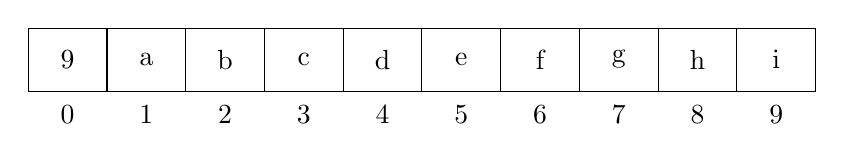
\begin{tikzpicture}
\draw (0,0) rectangle (10,0.8);
\foreach \x in {0,1,2,3,4,5,6,7,8,9}
    \draw (\x,0) -- (\x,0.8);
\node at (0.5,0.4) {9};
\node at (1.5,0.4) {a};
\node at (2.5,0.4) {b};
\node at (3.5,0.4) {c};
\node at (4.5,0.4) {d};
\node at (5.5,0.4) {e};
\node at (6.5,0.4) {f};
\node at (7.5,0.4) {g};
\node at (8.5,0.4) {h};
\node at (9.5,0.4) {i};
\node at (0.5,-0.3) {0};
\node at (1.5,-0.3) {1};
\node at (2.5,-0.3) {2};
\node at (3.5,-0.3) {3};
\node at (4.5,-0.3) {4};
\node at (5.5,-0.3) {5};
\node at (6.5,-0.3) {6};
\node at (7.5,-0.3) {7};
\node at (8.5,-0.3) {8};
\node at (9.5,-0.3) {9};
\end{tikzpicture}
\end{center}

\subsubsection{方法三:用结束符标记}

在串尾存储一个不会在串中出现的特殊字符作为字符串的终结符,例如,在C、C++和Java语言中用'\textbackslash 0'来表示串的结束。

\begin{center}
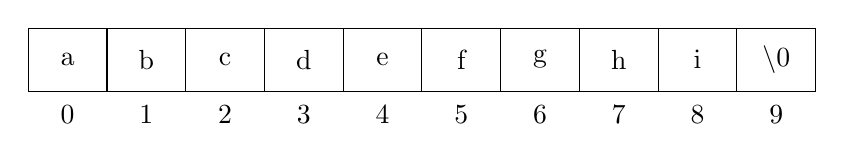
\begin{tikzpicture}
\draw (0,0) rectangle (10,0.8);
\foreach \x in {0,1,2,3,4,5,6,7,8,9}
    \draw (\x,0) -- (\x,0.8);
\node at (0.5,0.4) {a};
\node at (1.5,0.4) {b};
\node at (2.5,0.4) {c};
\node at (3.5,0.4) {d};
\node at (4.5,0.4) {e};
\node at (5.5,0.4) {f};
\node at (6.5,0.4) {g};
\node at (7.5,0.4) {h};
\node at (8.5,0.4) {i};
\node at (9.5,0.4) {\textbackslash 0};
\node at (0.5,-0.3) {0};
\node at (1.5,-0.3) {1};
\node at (2.5,-0.3) {2};
\node at (3.5,-0.3) {3};
\node at (4.5,-0.3) {4};
\node at (5.5,-0.3) {5};
\node at (6.5,-0.3) {6};
\node at (7.5,-0.3) {7};
\node at (8.5,-0.3) {8};
\node at (9.5,-0.3) {9};
\end{tikzpicture}
\end{center}

这种存储方法不能直接得到串的长度,而是通过判断当前字符是否为'\textbackslash 0'来确定串是否结束,从而求得串的长度。

\subsection{字符串的抽象数据类型定义}

字符串的逻辑结构与线性表的逻辑结构相同,但字符串的基本操作和线性表的基本操作有很大差别。线性表的基本操作大多以"单个元素"作为操作对象,而字符串的基本操作通常以"字符串整体"作为操作对象。

\begin{lstlisting}[caption=字符串抽象数据类型]
ADT String {
    数据对象:D = {ai | ai ∈ CharacterSet, i = 1,2,...,n, n ≥ 0}
    数据关系:R1 = {<ai-1, ai> | ai-1, ai ∈ D, i = 2,...,n}
    基本操作:
        StrAssign(T, chars);          // 串赋值
        StrCopy(T, S);               // 串复制
        StrEmpty(S);                 // 判断串空
        StrCompare(S, T);            // 串比较
        StrLength(S);                // 求串长
        StrConcat(T, S1, S2);        // 串连接
        SubString(Sub, S, pos, len); // 求子串
        Index(S, T, pos);            // 子串定位
        Replace(S, T, V);            // 串替换
        StrInsert(S, pos, T);        // 串插入
        StrDelete(S, pos, len);      // 串删除
} ADT String
\end{lstlisting}

\section{模式匹配算法}

模式匹配是字符串处理中最重要的操作之一。给定两个字符串 $S = "s_1s_2\cdots s_n"$ 和 $T = "t_1t_2\cdots t_m"$,在主串 $S$ 中寻找子串 $T$ 的过程称为模式匹配(pattern matching),$T$ 称为模式(pattern)。如果匹配成功,返回 $T$ 在 $S$ 中的位置;如果匹配失败,返回0。

\subsection{BF算法(暴力匹配)}

BF算法(Brute-Force algorithm)的基本思想是蛮力匹配,即从主串 $S$ 的第一个字符开始和模式 $T$ 的第一个字符进行比较。若相等,则继续比较两者的后续字符;否则,从主串 $S$ 的第二个字符开始和模式 $T$ 的第一个字符进行比较。重复上述过程,直至 $S$ 或 $T$ 中所有字符比较完毕。

\begin{algorithm}[H]
\caption{BF算法}
\begin{algorithmic}[1]
\REQUIRE 主串$S$,模式$T$
\ENSURE $T$在$S$中的位置
\STATE $start \leftarrow 0$, $i \leftarrow 0$, $j \leftarrow 0$
\WHILE{$S[i] \neq '\backslash 0'$ AND $T[j] \neq '\backslash 0'$}
    \IF{$S[i] = T[j]$}
        \STATE $i \leftarrow i + 1$, $j \leftarrow j + 1$
    \ELSE
        \STATE $start \leftarrow start + 1$
        \STATE $i \leftarrow start$, $j \leftarrow 0$
    \ENDIF
\ENDWHILE
\IF{$T[j] = '\backslash 0'$}
    \RETURN $start + 1$
\ELSE
    \RETURN $0$
\ENDIF
\end{algorithmic}
\end{algorithm}

\begin{lstlisting}[caption=BF算法C++实现]
int BF(char S[], char T[]) {
    int start = 0;  // 主串从下标0开始第一趟匹配
    int i = 0, j = 0;  // 设置比较的起始下标
    
    while (S[i] != '\0' && T[j] != '\0') {
        if (S[i] == T[j]) {
            i++; j++;  // 继续比较下一对字符
        } else {
            start++;   // 开始下一趟匹配
            i = start; j = 0;  // i和j分别回溯
        }
    }
    
    if (T[j] == '\0')
        return start + 1;  // 返回本趟匹配的起始位置
    else
        return 0;  // 匹配失败
}
\end{lstlisting}

\begin{theorem}[BF算法时间复杂度]
设主串 $S$ 长度为 $n$,模式 $T$ 长度为 $m$,在匹配成功的情况下,考虑两种极端情况:
\begin{enumerate}
\item \textbf{最好情况}:每趟不成功的匹配都发生在模式 $T$ 的第一个字符。平均比较次数为 $\frac{n+m}{2} = O(n+m)$。
\item \textbf{最坏情况}:每趟不成功的匹配都发生在模式 $T$ 的最后一个字符。平均比较次数为 $\frac{m(n-m+2)}{2} = O(n \times m)$。
\item \textbf{平均情况}:$O(n+m)$
\end{enumerate}
其中$n$为主串长度,$m$为模式长度。
\end{theorem}

\begin{example}[BF算法执行过程]
设主串 $S = "abcabcacb"$,模式 $T = "abcac"$,BF算法的匹配过程如下:

\textbf{第1趟匹配:}
\begin{center}
\begin{tabular}{|c|c|c|c|c|c|c|c|c|c|}
\hline
S & a & b & c & a & b & c & a & c & b \\
\hline
T & a & b & c & a & \textcolor{red}{c} &  &  &  &  \\
\hline
\end{tabular}
\end{center}
$i=4, j=4$ 失败,$i$ 回溯到1,$j$ 回溯到0

\textbf{第2趟匹配:}
\begin{center}
\begin{tabular}{|c|c|c|c|c|c|c|c|c|c|}
\hline
S & a & \textcolor{red}{b} & c & a & b & c & a & c & b \\
\hline
T &  & \textcolor{red}{a} &  &  &  &  &  &  &  \\
\hline
\end{tabular}
\end{center}
$i=1, j=0$ 失败,$i$ 回溯到2,$j$ 回溯到0

\textbf{第3趟匹配:}
\begin{center}
\begin{tabular}{|c|c|c|c|c|c|c|c|c|c|}
\hline
S & a & b & \textcolor{red}{c} & a & b & c & a & c & b \\
\hline
T &  &  & \textcolor{red}{a} &  &  &  &  &  &  \\
\hline
\end{tabular}
\end{center}
$i=2, j=0$ 失败,$i$ 回溯到3,$j$ 回溯到0

\textbf{第4趟匹配:}
\begin{center}
\begin{tabular}{|c|c|c|c|c|c|c|c|c|c|}
\hline
S & a & b & c & a & b & c & a & c & b \\
\hline
T &  &  &  & a & b & c & a & c &  \\
\hline
\end{tabular}
\end{center}
$i=8, j=5$,$T$ 中全部字符都比较完毕,匹配成功,返回位置4。
\end{example}

\subsection{KMP算法}

KMP算法是克努思(Knuth)、莫里斯(Morris)和普拉特(Pratt)同时设计的,是对BF算法的重大改进。KMP算法的核心思想是避免主串指针回溯,通过预计算模式的next数组实现高效匹配。

\subsubsection{KMP算法的基本思想}

分析BF算法的执行过程,造成BF算法效率低的原因是回溯,即在某趟匹配失败后,对于主串$S$要回溯到本趟匹配开始字符的下一个字符,模式$T$要回溯到第一个字符,而这些回溯往往是不必要的。

KMP算法希望某趟在$S[i]$和$T[j]$匹配失败后,下标$i$不回溯,下标$j$回溯至某个位置$k$,使得$T[k]$对准$S[i]$继续进行比较。关键问题是如何确定位置$k$。

\begin{definition}[next数组]
模式中的每一个字符$T[j]$都对应一个$k$值,这个$k$值仅依赖于模式本身,与主串无关。用$\text{next}[j]$表示$T[j]$对应的$k$值$(0 \leq j < m)$,其定义如下:
$$\text{next}[j] = \begin{cases}
-1 & j = 0 \\
\max\{k | 1 \leq k < j \text{ 且 } T[0]\cdots T[k-1] = T[j-k]\cdots T[j-1]\} & \text{集合非空} \\
0 & \text{其他情况}
\end{cases}$$
\end{definition}

\textbf{next数组的含义:}
next[j]表示当模式中第j个字符与主串中相应字符"失配"时,在模式中需要重新和主串中该字符进行比较的字符的位置。

\begin{example}[计算next数组]
设模式 $T = "ababc"$,计算其next值:

\begin{center}
\begin{tabular}{|c|c|c|c|c|c|}
\hline
j & 0 & 1 & 2 & 3 & 4 \\
\hline
T[j] & a & b & a & b & c \\
\hline
next[j] & -1 & 0 & 0 & 1 & 2 \\
\hline
\end{tabular}
\end{center}

计算过程:
\begin{itemize}
\item $j=0$: $\text{next}[0] = -1$
\item $j=1$: $\text{next}[1] = 0$
\item $j=2$: $T[0] \neq T[1]$,故 $\text{next}[2] = 0$
\item $j=3$: $T[0] = T[2] = a$,故 $\text{next}[3] = 1$
\item $j=4$: $T[0]T[1] = T[2]T[3] = ab$,故 $\text{next}[4] = 2$
\end{itemize}
\end{example}

\begin{example}[KMP算法执行过程]
设主串 $S = "ababcabcacbab"$,模式 $T = "abcac"$。

首先计算模式T的next数组。`next[j]` 的值是模式串 `T` 的子串 `T[0...j-1]` 的最长公共前后缀的长度。

\begin{center}
\begin{tabular}{|c|c|c|c|c|c|}
\hline
j & 0 & 1 & 2 & 3 & 4 \\
\hline
T[j] & a & b & c & a & c \\
\hline
next[j] & -1 & 0 & 0 & 0 & 1 \\
\hline
\end{tabular}
\end{center}
\textbf{详细计算过程}:
\begin{itemize}
    \item \textbf{j = 0}: 
        \begin{itemize}
            \item `next[0]` 按定义为 -1。这是一个哨兵值,表示模式串的第一个字符就不匹配,此时主串指针需要后移。
        \end{itemize}
    \item \textbf{j = 1}: 
        \begin{itemize}
            \item 子串 `T[0...0]` 为 "a"。
            \item 其所有前缀和后缀都为空。最长公共前后缀长度为0。
            \item 所以 `next[1] = 0`。
        \end{itemize}
    \item \textbf{j = 2}: 
        \begin{itemize}
            \item 子串 `T[0...1]` 为 "ab"。
            \item 前缀: \{"a"\}。后缀: \{"b"\}。
            \item 两者没有交集。最长公共前后缀长度为0。
            \item 所以 `next[2] = 0`。
        \end{itemize}
    \item \textbf{j = 3}: 
        \begin{itemize}
            \item 子串 `T[0...2]` 为 "abc"。
            \item 前缀: \{"a", "ab"\}。后缀: \{"c", "bc"\}。
            \item 两者没有交集。最长公共前后缀长度为0。
            \item 所以 `next[3] = 0`。
        \end{itemize}
    \item \textbf{j = 4}: 
        \begin{itemize}
            \item 子串 `T[0...3]` 为 "abca"。
            \item 前缀: \{"a", "ab", "abc"\}。后缀: \{"a", "ca", "bca"\}。
            \item 最长的公共元素是 "a",长度为1。
            \item 所以 `next[4] = 1`。
        \end{itemize}
\end{itemize}

\textbf{KMP匹配过程} (i为主串指针,j为模式串指针):

\textbf{第1趟匹配:} $i$从0开始, $j$从0开始
\begin{center}
\begin{tabular}{|c|c|c|c|c|c|c|c|c|c|c|c|c|}
\hline
S & a & b & c & a & \textcolor{red}{b} & c & a & c & b & a & b & \\
\hline
T & a & b & c & a & \textcolor{red}{c} &  &  &  &  &  &  &  \\
\hline
索引i & 0 & 1 & 2 & 3 & 4 & 5 & 6 & 7 & 8 & 9 & 10 & 11 \\
\hline
\end{tabular}
\end{center}
在 $i=4, j=4$ 时,$S[4]='b' \neq T[4]='c'$,发生不匹配。\\
根据KMP算法,主串指针$i$不回溯 ($i$保持为4),模式串指针$j$更新为 $j = \text{next}[4] = 1$。

\textbf{第2趟匹配:}
\begin{center}
\begin{tabular}{|c|c|c|c|c|c|c|c|c|c|c|c|c|}
\hline
S & a & b & c & a & \textcolor{red}{b} & c & a & c & b & a & b & \\
\hline
T &   &   &   &   & \textcolor{red}{b} & c & a & c &  &  &  &  \\
\hline
索引i & 0 & 1 & 2 & 3 & 4 & 5 & 6 & 7 & 8 & 9 & 10 & 11 \\
\hline
\end{tabular}
\end{center}
从 $i=4, j=1$ 继续比较。$S[4]='b' = T[1]='b'$,匹配。$i,j$ 都加1。\\
$i=5, j=2$ 时,$S[5]='c' = T[2]='c'$,匹配。$i,j$ 都加1。\\
$i=6, j=3$ 时,$S[6]='a' = T[3]='a'$,匹配。$i,j$ 都加1。\\
$i=7, j=4$ 时,$S[7]='c' = T[4]='c'$,匹配。$i,j$ 都加1。\\
$i=8, j=5$ 时,$T[j]$ 到达末尾($\backslash 0$),说明匹配成功。\\
返回匹配开始的位置 $i-j = 8-5 = 3$ (若从1开始计数,则是位置4)。
\end{example}

\begin{algorithm}
\caption{KMP算法}
\begin{algorithmic}[1]
\REQUIRE 主串$S$,模式$T$,next数组
\ENSURE $T$在$S$中的位置
\STATE $i \leftarrow 0$, $j \leftarrow 0$
\WHILE{$S[i] \neq '\backslash 0'$ AND $T[j] \neq '\backslash 0'$}
    \IF{$S[i] = T[j]$}
        \STATE $i \leftarrow i + 1$, $j \leftarrow j + 1$
    \ELSE
        \STATE $j \leftarrow \text{next}[j]$
        \IF{$j = -1$}
            \STATE $i \leftarrow i + 1$, $j \leftarrow 0$
        \ENDIF
    \ENDIF
\ENDWHILE
\IF{$T[j] = '\backslash 0'$}
    \RETURN $i - j + 1$
\ELSE
    \RETURN $0$
\ENDIF
\end{algorithmic}
\end{algorithm}

\begin{theorem}[KMP算法时间复杂度]
KMP算法的时间复杂度为 $O(n+m)$,其中$n$为主串长度,$m$为模式长度。
\end{theorem}

\section{多维数组}

\subsection{数组的基本概念}

\begin{definition}[数组]
数组是由类型相同的数据元素构成的有序集合,每个元素受$n(n \geq 1)$个线性关系约束,每个元素在$n$个线性关系中的序号称为下标。
\end{definition}

数组的特点:
\begin{itemize}
\item 数据元素类型相同
\item 结构固定,一般不做插入删除操作
\item 支持随机访问
\item 是线性表的推广
\end{itemize}

\subsection{数组的存储结构与寻址}

\subsubsection{二维数组的存储}

二维数组可按两种方式存储:
\begin{itemize}
\item \textbf{按行优先}:先行后列存储
\item \textbf{按列优先}:先列后行存储
\end{itemize}

\begin{theorem}[二维数组按行优先寻址公式]
设二维数组$A[l_1..h_1][l_2..h_2]$,按行优先存储,则元素$a_{ij}$的地址为:
$$\text{LOC}(a_{ij}) = \text{LOC}(a_{l_1l_2}) + [(i-l_1) \times (h_2-l_2+1) + (j-l_2)] \times c$$
其中$c$为每个元素占用的存储单元数。
\end{theorem}

\subsubsection{多维数组的寻址}

对于$n$维数组$A[d_1][d_2]\cdots[d_n]$,按行优先存储,元素$A[i_1][i_2]\cdots[i_n]$的地址为:
$$\text{LOC}(A[i_1][i_2]\cdots[i_n]) = \text{LOC}(A[0][0]\cdots[0]) + \left(\sum_{k=1}^{n} i_k \prod_{j=k+1}^{n} d_j\right) \times c$$

\section{矩阵的压缩存储}

\subsection{特殊矩阵的压缩存储}

\subsubsection{对称矩阵}

对称矩阵满足 $a_{ij} = a_{ji}$,只需存储下三角部分。

\begin{theorem}[对称矩阵寻址公式]
$n$阶对称矩阵按行优先存储下三角部分,元素$a_{ij}$在一维数组中的下标为:
$$k = \begin{cases}
\frac{i(i-1)}{2} + j - 1 & \text{if } i \geq j \\
\frac{j(j-1)}{2} + i - 1 & \text{if } i < j
\end{cases}$$
\end{theorem}

\subsubsection{三角矩阵}

\begin{itemize}
\item \textbf{下三角矩阵}:主对角线以上元素为常数$c$
\item \textbf{上三角矩阵}:主对角线以下元素为常数$c$
\end{itemize}

存储方案:存储非常数元素 + 一个常数。

\subsubsection{对角矩阵(带状矩阵)}

对角矩阵的非零元素集中在主对角线及其附近的几条对角线上。

\begin{example}[三对角矩阵]
三对角矩阵的寻址公式:
$$k = 2i + j - 3 \quad (|i-j| \leq 1)$$
\end{example}

\subsection{稀疏矩阵的存储}

\begin{definition}[稀疏矩阵]
设$m \times n$矩阵中有$t$个非零元素,若$t \ll m \times n$,则称该矩阵为稀疏矩阵。
\end{definition}

稀疏矩阵的存储策略:只存储非零元素,节省存储空间。

\subsubsection{三元组表示法}

三元组$(i, j, v)$表示矩阵第$i$行第$j$列的元素值为$v$。

\begin{lstlisting}[caption=三元组结构定义]
typedef struct {
    int i, j;        // 行号和列号
    ElemType e;      // 元素值
} Triple;

typedef struct {
    Triple data[MAXSIZE];  // 三元组表
    int m, n, t;          // 矩阵的行数、列数和非零元素个数
} TSMatrix;
\end{lstlisting}

\subsubsection{稀疏矩阵的转置}

\textbf{方法一:简单转置算法}

\begin{algorithm}[H]
\caption{简单转置算法}
\begin{algorithmic}[1]
\REQUIRE 稀疏矩阵$A$
\ENSURE 转置矩阵$B$
\STATE $B.m \leftarrow A.n$, $B.n \leftarrow A.m$, $B.t \leftarrow A.t$
\STATE $q \leftarrow 1$
\FOR{$col = 1$ to $A.n$}
    \FOR{$p = 1$ to $A.t$}
        \IF{$A.data[p].j = col$}
            \STATE $B.data[q].i \leftarrow A.data[p].j$
            \STATE $B.data[q].j \leftarrow A.data[p].i$
            \STATE $B.data[q].e \leftarrow A.data[p].e$
            \STATE $q \leftarrow q + 1$
        \ENDIF
    \ENDFOR
\ENDFOR
\end{algorithmic}
\end{algorithm}

\begin{theorem}[简单转置算法时间复杂度]
时间复杂度为$O(n \times t)$,其中$n$为矩阵列数,$t$为非零元素个数。当$t$与$m \times n$同数量级时,算法的时间复杂度为$O(m \times n^2)$。
\end{theorem}

\textbf{方法二:快速转置算法}

利用辅助数组记录每列的非零元素个数和每列第一个非零元素在转置矩阵中的位置。

\begin{algorithm}[H]
\caption{快速转置算法}
\begin{algorithmic}[1]
\REQUIRE 稀疏矩阵$A$
\ENSURE 转置矩阵$B$
\STATE $B.m \leftarrow A.n$, $B.n \leftarrow A.m$, $B.t \leftarrow A.t$
\STATE 初始化$num[1..A.n]$和$cpot[1..A.n]$
\FOR{$col = 1$ to $A.n$}
    \STATE $num[col] \leftarrow 0$
\ENDFOR
\FOR{$t = 1$ to $A.t$}
    \STATE $num[A.data[t].j] \leftarrow num[A.data[t].j] + 1$
\ENDFOR
\STATE $cpot[1] \leftarrow 1$
\FOR{$col = 2$ to $A.n$}
    \STATE $cpot[col] \leftarrow cpot[col-1] + num[col-1]$
\ENDFOR
\FOR{$p = 1$ to $A.t$}
    \STATE $col \leftarrow A.data[p].j$
    \STATE $pos \leftarrow cpot[col]$
    \STATE $B.data[pos] \leftarrow$ 转置$A.data[p]$
    \STATE $cpot[col] \leftarrow cpot[col] + 1$
\ENDFOR
\end{algorithmic}
\end{algorithm}

\begin{theorem}[快速转置算法时间复杂度]
时间复杂度为$O(n + t)$,其中$n$为矩阵列数,$t$为非零元素个数。
\end{theorem}

\subsubsection{十字链表表示法}

对于频繁进行插入、删除操作的稀疏矩阵,三元组表示法效率较低,可采用十字链表表示法。

\begin{lstlisting}[caption=十字链表结构定义]
typedef struct OLNode {
    int i, j;                    // 行号和列号
    ElemType e;                  // 元素值
    struct OLNode *right, *down; // 同行右邻接和同列下邻接
} OLNode, *OLink;

typedef struct {
    OLink *rhead, *chead;  // 行和列链表头指针向量
    int m, n, t;          // 矩阵的行数、列数和非零元素个数
} CrossList;
\end{lstlisting}

十字链表的优点:
\begin{itemize}
\item 能够方便地进行按行或按列遍历
\item 插入和删除操作效率高
\item 适合于矩阵运算
\end{itemize}

\subsubsection{稀疏矩阵转置算法详细示例}

设有如下$6 \times 7$稀疏矩阵$A$,包含7个非零元素:

$$
A = \begin{pmatrix}
0 & 0 & 12 & 0 & 9 & 0 & 0 \\
0 & 0 & 0 & 0 & 0 & 0 & 0 \\
0 & -1 & 0 & 0 & 0 & 0 & 0 \\
5 & 0 & 0 & -3 & 0 & 0 & 0 \\
0 & 0 & 0 & 0 & 0 & 2 & 0 \\
0 & 0 & 0 & 0 & 8 & 0 & 0
\end{pmatrix}
$$

三元组表示为:$A.m = 6$,$A.n = 7$,$A.t = 7$

\begin{center}
\begin{tabular}{|c|c|c|c|}
\hline
p(下标) & i(行) & j(列) & e(值) \\
\hline
1 & 1 & 3 & 12 \\
2 & 1 & 5 & 9 \\
3 & 3 & 2 & -1 \\
4 & 4 & 1 & 5 \\
5 & 4 & 4 & -3 \\
6 & 5 & 6 & 2 \\
7 & 6 & 5 & 8 \\
\hline
\end{tabular}
\end{center}

\textbf{例:简单转置算法执行过程}

初始化:$B.m = 7$,$B.n = 6$,$B.t = 7$,$q = 1$

\begin{enumerate}
\item \textbf{col = 1}:扫描$A.data$,找到$A.data[4]$的$j=1$
    \begin{itemize}
    \item 转置$(4, 1, 5) \rightarrow (1, 4, 5)$
    \item 存入$B.data[1]$,$q = 2$
    \end{itemize}

\item \textbf{col = 2}:扫描$A.data$,找到$A.data[3]$的$j=2$
    \begin{itemize}
    \item 转置$(3, 2, -1) \rightarrow (2, 3, -1)$
    \item 存入$B.data[2]$,$q = 3$
    \end{itemize}

\item \textbf{col = 3}:扫描$A.data$,找到$A.data[1]$的$j=3$
    \begin{itemize}
    \item 转置$(1, 3, 12) \rightarrow (3, 1, 12)$
    \item 存入$B.data[3]$,$q = 4$
    \end{itemize}

\item \textbf{col = 4}:扫描$A.data$,找到$A.data[5]$的$j=4$
    \begin{itemize}
    \item 转置$(4, 4, -3) \rightarrow (4, 4, -3)$
    \item 存入$B.data[4]$,$q = 5$
    \end{itemize}

\item \textbf{col = 5}:扫描$A.data$,找到两个元素$j=5$
    \begin{itemize}
    \item 转置$(1, 5, 9) \rightarrow (5, 1, 9)$,存入$B.data[5]$,$q = 6$
    \item 转置$(6, 5, 8) \rightarrow (5, 6, 8)$,存入$B.data[6]$,$q = 7$
    \end{itemize}

\item \textbf{col = 6}:扫描$A.data$,找到$A.data[6]$的$j=6$
    \begin{itemize}
    \item 转置$(5, 6, 2) \rightarrow (6, 5, 2)$
    \item 存入$B.data[7]$,$q = 8$
    \end{itemize}

\item \textbf{col = 7}:扫描$A.data$,无元素
\end{enumerate}

\textbf{最终结果$B.data$:}

\begin{center}
\begin{tabular}{|c|c|c|c|}
\hline
q(下标) & i(行) & j(列) & e(值) \\
\hline
1 & 1 & 4 & 5 \\
2 & 2 & 3 & -1 \\
3 & 3 & 1 & 12 \\
4 & 4 & 4 & -3 \\
5 & 5 & 1 & 9 \\
6 & 5 & 6 & 8 \\
7 & 6 & 5 & 2 \\
\hline
\end{tabular}
\end{center}

\textbf{例:快速转置算法执行过程}

\textbf{步骤1:计算num数组}

$num[col]$存储$A$的第$col$列的非零元素个数。扫描$A.data$一次:

\begin{center}
\begin{tabular}{|c|c|c|c|c|c|c|c|}
\hline
col & 1 & 2 & 3 & 4 & 5 & 6 & 7 \\
\hline
num & 1 & 1 & 1 & 1 & 2 & 1 & 0 \\
\hline
\end{tabular}
\end{center}

\textbf{步骤2:计算cpot数组}

$cpot[col]$存储$A$的第$col$列元素在$B.data$中的起始位置:

\begin{align}
cpot[1] &= 1 \\
cpot[2] &= cpot[1] + num[1] = 1 + 1 = 2 \\
cpot[3] &= cpot[2] + num[2] = 2 + 1 = 3 \\
cpot[4] &= cpot[3] + num[3] = 3 + 1 = 4 \\
cpot[5] &= cpot[4] + num[4] = 4 + 1 = 5 \\
cpot[6] &= cpot[5] + num[5] = 5 + 2 = 7 \\
cpot[7] &= cpot[6] + num[6] = 7 + 1 = 8
\end{align}

\begin{center}
\begin{tabular}{|c|c|c|c|c|c|c|c|}
\hline
col & 1 & 2 & 3 & 4 & 5 & 6 & 7 \\
\hline
cpot & 1 & 2 & 3 & 4 & 5 & 7 & 8 \\
\hline
\end{tabular}
\end{center}

\textbf{步骤3:放置元素到$B.data$}

最后一次扫描$A.data$,对每个元素$A.data[p]$:

\begin{enumerate}
\item \textbf{p = 1}:$A.data[1] = (1, 3, 12)$,$col=3$,$pos = cpot[3] = 3$
    \begin{itemize}
    \item 放置$(3, 1, 12)$到$B.data[3]$
    \item $cpot[3] \leftarrow 4$
    \end{itemize}

\item \textbf{p = 2}:$A.data[2] = (1, 5, 9)$,$col=5$,$pos = cpot[5] = 5$
    \begin{itemize}
    \item 放置$(5, 1, 9)$到$B.data[5]$
    \item $cpot[5] \leftarrow 6$
    \end{itemize}

\item \textbf{p = 3}:$A.data[3] = (3, 2, -1)$,$col=2$,$pos = cpot[2] = 2$
    \begin{itemize}
    \item 放置$(2, 3, -1)$到$B.data[2]$
    \item $cpot[2] \leftarrow 3$
    \end{itemize}

\item \textbf{p = 4}:$A.data[4] = (4, 1, 5)$,$col=1$,$pos = cpot[1] = 1$
    \begin{itemize}
    \item 放置$(1, 4, 5)$到$B.data[1]$
    \item $cpot[1] \leftarrow 2$
    \end{itemize}

\item \textbf{p = 5}:$A.data[5] = (4, 4, -3)$,$col=4$,$pos = cpot[4] = 4$
    \begin{itemize}
    \item 放置$(4, 4, -3)$到$B.data[4]$
    \item $cpot[4] \leftarrow 5$
    \end{itemize}

\item \textbf{p = 6}:$A.data[6] = (5, 6, 2)$,$col=6$,$pos = cpot[6] = 7$
    \begin{itemize}
    \item 放置$(6, 5, 2)$到$B.data[7]$
    \item $cpot[6] \leftarrow 8$
    \end{itemize}

\item \textbf{p = 7}:$A.data[7] = (6, 5, 8)$,$col=5$,$pos = cpot[5] = 6$
    \begin{itemize}
    \item 放置$(5, 6, 8)$到$B.data[6]$
    \item $cpot[5] \leftarrow 7$
    \end{itemize}
\end{enumerate}

\textbf{最终$B.data$结果:}

\begin{center}
\begin{tabular}{|c|c|c|c|}
\hline
q(下标) & i(行) & j(列) & e(值) \\
\hline
1 & 1 & 4 & 5 \\
2 & 2 & 3 & -1 \\
3 & 3 & 1 & 12 \\
4 & 4 & 4 & -3 \\
5 & 5 & 1 & 9 \\
6 & 5 & 6 & 8 \\
7 & 6 & 5 & 2 \\
\hline
\end{tabular}
\end{center}

两种算法得到相同的结果,但快速转置算法通过预计算避免了重复扫描,大大提高了效率。

\begin{lstlisting}[caption=快速转置算法C++实现]
void FastTranspose(TSMatrix A, TSMatrix &B) {
    B.m = A.n; B.n = A.m; B.t = A.t;
    
    int num[A.n + 1];  // 各列非零元个数
    int cpot[A.n + 1]; // 各列第一个非零元在B中的位置
    
    // 初始化num数组
    for (int col = 1; col <= A.n; col++)
        num[col] = 0;
    
    // 统计各列非零元个数
    for (int t = 1; t <= A.t; t++)
        num[A.data[t].j]++;
    
    // 计算各列第一个非零元在B中的位置
    cpot[1] = 1;
    for (int col = 2; col <= A.n; col++)
        cpot[col] = cpot[col-1] + num[col-1];
    
    // 转置
    for (int p = 1; p <= A.t; p++) {
        int col = A.data[p].j;
        int pos = cpot[col];
        B.data[pos].i = A.data[p].j;
        B.data[pos].j = A.data[p].i;
        B.data[pos].e = A.data[p].e;
        cpot[col]++;
    }
}
\end{lstlisting}

\section{广义表}

\subsection{广义表的定义}

\begin{definition}[广义表]
广义表(Generalized List)是$n(n \geq 0)$个元素的有限序列,记作:
$$LS = (a_1, a_2, \ldots, a_n)$$
其中$LS$是广义表的名称,$a_i$可以是原子或子表。
\end{definition}

\subsection{广义表的特性}

\begin{enumerate}
\item \textbf{有序性}:元素有先后次序
\item \textbf{长度}:最外层包含元素的个数
\item \textbf{深度}:括号的重数
\item \textbf{递归性}:广义表可以为自身的子表
\item \textbf{共享性}:可以被其他广义表所共享
\end{enumerate}

\begin{example}[广义表示例]
\begin{align}
A &= () && \text{空表,长度为0,深度为1} \\
B &= (e) && \text{长度为1,深度为1} \\
C &= (a, (b, c)) && \text{长度为2,深度为2} \\
D &= (a, b, (c, d), e) && \text{长度为4,深度为2} \\
E &= ((a, b), (c, d)) && \text{长度为2,深度为2} \\
F &= (a, F) && \text{递归定义,长度为2,深度无穷}
\end{align}
\end{example}

\subsection{广义表的存储结构}

\subsubsection{头尾链表存储}

\indent

\begin{lstlisting}[caption=头尾链表结构定义]
typedef enum {ATOM, LIST} ElemTag;

typedef struct GLNode {
    ElemTag tag;           // 标志域:ATOM或LIST
    union {
        AtomType atom;     // 原子结点的值域
        struct {
            struct GLNode *hp, *tp;  // 表结点的指针域,hp指向表头,tp指向表尾
        } ptr;
    };
} *GList;
\end{lstlisting}

\subsubsection{子表结点存储}

\indent

\begin{lstlisting}[caption=子表结点结构定义]
typedef struct GLNode {
    ElemTag tag;
    union {
        AtomType atom;
        struct GLNode *hp;  // 指向子表
    };
    struct GLNode *tp;      // 指向同层下一个结点
} *GList;
\end{lstlisting}

\subsection{广义表的基本操作}

\textbf{求广义表的长度:}
\begin{lstlisting}[caption=求广义表长度]
int GListLength(GList L) {
    if (!L) return 0;
    int len = 0;
    while (L) {
        len++;
        L = L->tp;
    }
    return len;
}
\end{lstlisting}

\textbf{求广义表的深度:}
\begin{lstlisting}[caption=求广义表深度]
int GListDepth(GList L) {
    if (!L) return 1;     // 空表深度为1
    if (L->tag == ATOM) return 0;  // 原子深度为0
    
    int maxdep = 0;
    while (L) {
        if (L->tag == LIST) {
            int dep = GListDepth(L->ptr.hp);
            if (dep > maxdep) maxdep = dep;
        }
        L = L->ptr.tp;
    }
    return maxdep + 1;
}
\end{lstlisting}

\subsection{稀疏矩阵的压缩存储}

稀疏矩阵是零元素很多的矩阵,稀疏因子$\delta = \frac{t}{m \times n} < 0.05$。

\subsubsection{三元组顺序表}

将非零元素表示为三元组$(i, j, a_{ij})$,按行优先顺序存储。

\begin{verbatim}
struct Element {
    int row, col;
    DataType value;
};

struct SparseMatrix {
    Element data[MaxSize];
    int rows, cols, nums;  // 行数、列数、非零元个数
};
\end{verbatim}

\subsubsection{十字链表}

每个非零元素节点包含5个域:row, col, value, right, down。
\begin{itemize}
\item right指向同行下一个非零元素
\item down指向同列下一个非零元素
\end{itemize}

\subsection{稀疏矩阵转置算法}

\subsubsection{转置算法1(直接转置)}

\begin{algorithm}
\caption{稀疏矩阵转置算法1}
\begin{algorithmic}[1]
\REQUIRE 稀疏矩阵$A$
\ENSURE 转置矩阵$B$
\STATE 设置$B$的行数、列数、非零元个数
\FOR{$col = 1$ to $A.cols$}
    \FOR{$i = 0$ to $A.nums-1$}
        \IF{$A.data[i].col = col$}
            \STATE 将$A.data[i]$行列交换后存入$B$
        \ENDIF
    \ENDFOR
\ENDFOR
\end{algorithmic}
\end{algorithm}

时间复杂度:$O(cols \times nums)$

\subsubsection{转置算法2(快速转置)}

引入辅助数组:
\begin{itemize}
\item $num[1..A.n]$:第$col$列非零元个数
\item $cpot[1..A.n]$:第$col$列第一个非零元在$B$中的位置
\end{itemize}

递推关系:
$$\begin{cases}
cpot[1] = 0 \\
cpot[col] = cpot[col-1] + num[col-1] \quad (2 \leq col \leq nu)
\end{cases}$$

\begin{algorithm}
\caption{稀疏矩阵转置算法2}
\begin{algorithmic}[1]
\REQUIRE 稀疏矩阵$A$
\ENSURE 转置矩阵$B$
\STATE 统计每列非零元个数到$num[]$
\STATE 计算每列第一个元素在$B$中位置到$cpot[]$
\FOR{$i = 0$ to $A.nums-1$}
    \STATE $col \leftarrow A.data[i].col$
    \STATE $pos \leftarrow cpot[col]$
    \STATE $B.data[pos] \leftarrow$ 转置$A.data[i]$
    \STATE $cpot[col] \leftarrow cpot[col] + 1$
\ENDFOR
\end{algorithmic}
\end{algorithm}

时间复杂度:$O(cols + nums)$

\section{重难点分析}

\subsection{重点内容}
\begin{enumerate}
\item \textbf{模式匹配算法}(★★★★★)
    \begin{itemize}
    \item BF算法的执行过程和复杂度分析
    \item KMP算法的next数组计算
    \item KMP算法的匹配过程
    \end{itemize}
    
\item \textbf{数组寻址公式}(★★★★☆)
    \begin{itemize}
    \item 二维数组按行/列优先的寻址公式
    \item 多维数组的寻址公式推导
    \end{itemize}
    
\item \textbf{特殊矩阵压缩存储}(★★★★☆)
    \begin{itemize}
    \item 对称矩阵的存储和寻址
    \item 三角矩阵的存储方案
    \item 对角矩阵的压缩存储
    \end{itemize}
\end{enumerate}

\subsection{难点内容}
\begin{enumerate}
\item \textbf{KMP算法的next数组计算}(★★★★★)
    \begin{itemize}
    \item 理解next数组的含义
    \item 掌握手工计算next值的方法
    \item 理解KMP算法避免回溯的原理
    \end{itemize}
    
\item \textbf{稀疏矩阵的压缩存储}(★★★★☆)
    \begin{itemize}
    \item 三元组表的组织方式
    \item 十字链表的结构设计
    \item 稀疏矩阵转置算法的优化
    \end{itemize}
\end{enumerate}


\section{典型例题}

\begin{example}[KMP算法next数组计算]
设模式串$T = "abcabca"$,求其next数组。

\textbf{解答:}
\begin{center}
\begin{tabular}{|c|c|c|c|c|c|c|c|}
\hline
j & 0 & 1 & 2 & 3 & 4 & 5 & 6 \\
\hline
T[j] & a & b & c & a & b & c & a \\
\hline
next[j] & -1 & 0 & 0 & 0 & 1 & 2 & 3 \\
\hline
\end{tabular}
\end{center}

计算过程:
\begin{itemize}
\item $j=0$: $\text{next}[0] = -1$
\item $j=1$: $\text{next}[1] = 0$
\item $j=2$: $T[0] \neq T[1]$,$\text{next}[2] = 0$
\item $j=3$: $T[0] \neq T[1] \neq T[2]$,$\text{next}[3] = 0$
\item $j=4$: $T[0] = T[3] = a$,$\text{next}[4] = 1$
\item $j=5$: $T[0]T[1] = T[3]T[4] = ab$,$\text{next}[5] = 2$
\item $j=6$: $T[0]T[1]T[2] = T[3]T[4]T[5] = abc$,$\text{next}[6] = 3$
\end{itemize}
\end{example}

\begin{example}[对称矩阵压缩存储]
设有5阶对称矩阵,按行优先存储下三角部分,求元素$a_{32}$和$a_{23}$在一维数组中的下标。

\textbf{解答:}
对于$a_{32}$($i=3, j=2$),由于$i > j$,直接计算:
$$k = \frac{i(i-1)}{2} + j - 1 = \frac{3 \times 2}{2} + 2 - 1 = 4$$

对于$a_{23}$($i=2, j=3$),由于$i < j$,利用对称性$a_{23} = a_{32}$:
$$k = \frac{j(j-1)}{2} + i - 1 = \frac{3 \times 2}{2} + 2 - 1 = 4$$

因此两个元素都存储在下标4的位置。
\end{example}

\begin{example}[二维数组寻址]
设有二维数组$A[1..10][5..15]$,每个元素占4个字节,按行优先存储,数组首地址为1000,求$A[5][8]$的地址。

\textbf{解答:}
按行优先寻址公式:
$$\text{LOC}(A[i][j]) = \text{LOC}(A[1][5]) + [(i-1) \times (15-5+1) + (j-5)] \times 4$$

代入$i=5, j=8$:
$$\text{LOC}(A[5][8]) = 1000 + [(5-1) \times 11 + (8-5)] \times 4$$
$$= 1000 + (44 + 3) \times 4 = 1000 + 188 = 1188$$
\end{example}

\section{复习建议}

\subsection{学习重点顺序}
\begin{enumerate}
\item \textbf{第一轮:掌握基本概念}
    \begin{itemize}
    \item 字符串的定义和存储方式
    \item 数组的寻址计算方法
    \item 矩阵压缩存储的基本思想
    \end{itemize}
    
\item \textbf{第二轮:理解核心算法}
    \begin{itemize}
    \item BF算法的执行过程
    \item KMP算法的next数组计算
    \item 稀疏矩阵的转置算法
    \end{itemize}
    
\item \textbf{第三轮:强化练习}
    \begin{itemize}
    \item 大量next数组计算练习
    \item 各种寻址公式的推导和应用
    \item 算法复杂度分析
    \end{itemize}
\end{enumerate}

\subsection{常考题型}
\begin{enumerate}
\item \textbf{选择题}:算法复杂度、存储效率、概念理解
\item \textbf{填空题}:next数组数值、寻址公式结果、复杂度表达式
\item \textbf{应用题}:手工执行算法、公式推导、程序设计
\item \textbf{算法题}:KMP算法实现、矩阵操作算法
\end{enumerate}

\subsection{记忆要点}
\begin{enumerate}
\item \textbf{KMP算法}:
    \begin{itemize}
    \item next[0] = -1, next[1] = 0
    \item 寻找最长相同前缀后缀
    \item 时间复杂度O(m+n)
    \end{itemize}
    
\item \textbf{寻址公式}:
    \begin{itemize}
    \item 二维数组:LOC = base + (i×列数 + j)×size
    \item 对称矩阵:k = i(i-1)/2 + j - 1(i≥j)
    \item 三角矩阵:存储方式决定公式形式
    \end{itemize}
    
\item \textbf{复杂度}:
    \begin{itemize}
    \item BF算法:最坏O(mn),平均O(m+n)
    \item KMP算法:O(m+n)
    \item 矩阵转置:简单O(列数×非零元),快速O(列数+非零元)
    \end{itemize}
\end{enumerate}

\section{扩展知识}

\subsection{高级字符串算法}
\begin{itemize}
\item \textbf{Boyer-Moore算法}:从右向左匹配,使用坏字符和好后缀规则
\item \textbf{Sunday算法}:BM算法的简化版本,使用坏字符规则
\item \textbf{Rabin-Karp算法}:基于哈希值的匹配算法
\item \textbf{AC自动机}:多模式串匹配,基于KMP和字典树
\end{itemize}

\subsection{现代应用}
\begin{itemize}
\item \textbf{文本编辑器}:查找替换功能的核心算法
\item \textbf{生物信息学}:DNA序列分析中的模式匹配
\item \textbf{信息检索}:搜索引擎中的字符串匹配
\item \textbf{网络安全}:入侵检测系统中的模式识别
\end{itemize}

\subsection{相关数据结构}
\begin{itemize}
\item \textbf{字典树(Trie)}:高效的字符串存储和检索
\item \textbf{后缀数组}:字符串处理的强大工具
\item \textbf{后缀树}:线性时间的多种字符串操作
\item \textbf{压缩索引}:大数据时代的字符串索引技术
\end{itemize}

\section{总结}

字符串和多维数组是数据结构中的重要内容,具有很强的实用性。学习重点包括:

\begin{enumerate}
\item \textbf{理论基础}:深入理解各种算法的原理和适用场景
\item \textbf{算法实现}:熟练掌握关键算法的实现细节
\item \textbf{复杂度分析}:能够准确分析算法的时间空间复杂度
\item \textbf{实际应用}:了解这些数据结构在实际项目中的应用
\end{enumerate}

通过系统学习和大量练习,相信同学们能够很好地掌握这部分内容,为后续课程和实际应用打下坚实基础。

\end{document}

\section{复习建议}

\begin{mdframed}[style=framestyle]
\subsection{学习重点}
\begin{enumerate}
\item \textbf{熟练掌握KMP算法}
    \begin{itemize}
    \item 多练习next数组的手工计算
    \item 理解KMP算法的匹配过程
    \item 掌握算法的时间复杂度分析
    \end{itemize}
    
\item \textbf{掌握数组寻址公式}
    \begin{itemize}
    \item 记忆二维数组的寻址公式
    \item 理解行优先和列优先的区别
    \item 练习多维数组的寻址计算
    \end{itemize}
    
\item \textbf{掌握矩阵压缩存储}
    \begin{itemize}
    \item 理解各种特殊矩阵的特点
    \item 掌握压缩存储的寻址方法
    \item 理解稀疏矩阵的存储结构
    \end{itemize}
\end{enumerate}

\subsection{常考题型}
\begin{enumerate}
\item KMP算法的next数组计算
\item 数组元素的寻址计算
\item 特殊矩阵的压缩存储方案
\item 稀疏矩阵的存储结构设计
\item 字符串基本操作的实现
\end{enumerate}
\end{mdframed}

\section{扩展知识}

\subsection{字符串匹配的其他算法}
\begin{itemize}
\item \textbf{Boyer-Moore算法}:从右向左匹配,利用坏字符和好后缀规则
\item \textbf{Rabin-Karp算法}:基于哈希的字符串匹配
\item \textbf{Sunday算法}:BM算法的简化版本
\end{itemize}

\subsection{多维数组的应用}
\begin{itemize}
\item \textbf{图像处理}:二维数组表示图像像素
\item \textbf{科学计算}:多维数组表示张量
\item \textbf{动态规划}:多维数组存储状态
\end{itemize}

\subsection{压缩存储的实际应用}
\begin{itemize}
\item \textbf{大规模科学计算}:稀疏矩阵运算
\item \textbf{图论算法}:邻接矩阵的压缩存储
\item \textbf{机器学习}:特征矩阵的稀疏表示
\end{itemize}

\end{document} 
\part{二叉树}
\documentclass[12pt,a4paper]{amsart}
\usepackage[utf8]{inputenc}
\usepackage[T1]{fontenc}
\usepackage{amsmath,amsfonts,amssymb}
\usepackage{tikz}
\usepackage{algorithm}
\usepackage{algorithmic}
\usepackage{float}
\usepackage{listings}
\usepackage{xcolor}
\usepackage{geometry}
\usepackage{fancyhdr}
\usepackage{enumitem}
\usepackage{booktabs}
\usepackage{multirow}
\usepackage[hidelinks,bookmarksnumbered,bookmarksopen]{hyperref}
\usepackage{xeCJK}
\setCJKmainfont{LXGW WenKai}

\geometry{left=2.5cm,right=2.5cm,top=2.5cm,bottom=2.5cm}

% 代码高亮设置
\lstset{
    language=C++,
    basicstyle=\ttfamily\small,
    keywordstyle=\color{blue}\bfseries,
    commentstyle=\color{green!60!black},
    stringstyle=\color{red},
    numbers=left,
    numberstyle=\tiny\color{gray},
    stepnumber=1,
    numbersep=10pt,
    backgroundcolor=\color{gray!10},
    frame=single,
    tabsize=4,
    captionpos=b,
    breaklines=true,
    breakatwhitespace=false,
    showspaces=false,
    showstringspaces=false,
    showtabs=false
}

% 定理环境
\newtheorem{definition}{定义}[section]
\newtheorem{theorem}{定理}[section]

\newtheorem{example}{例题}[section]
\newtheorem{property}{性质}[section]

% TikZ库
\usetikzlibrary{trees,positioning,arrows,automata,calc}

\title{\textbf{数据结构 - 二叉树复习资料}}
\author{详细版本}
\date{\today}

\begin{document}

% \maketitle

% % 目录设置
% \tableofcontents
% \newpage

\section{二叉树的基本概念}

\subsection{树和二叉树的定义}

\begin{definition}[树]
树是$n(n \geq 0)$个结点的有限集合。当$n=0$时,称为空树;任意一棵非空树满足以下条件:
\begin{enumerate}
\item 有且仅有一个特定的称为根的结点;
\item 当$n>1$时,除根结点之外的其余结点被分成$m(m>0)$个互不相交的有限集合$T_1, T_2, \ldots, T_m$,其中每个集合又是一棵树,并称为这个根结点的子树。
\end{enumerate}
\end{definition}

\begin{definition}[二叉树]
二叉树是$n(n \geq 0)$个结点的有限集合,该集合或者为空集(称为空二叉树),或者由一个根结点和两棵互不相交的、分别称为根结点的左子树和右子树的二叉树组成。
\end{definition}

\subsection{二叉树的特点}

二叉树具有以下特点:
\begin{enumerate}
\item 每个结点最多有两棵子树,所以二叉树中不存在度大于2的结点;
\item 二叉树的左右子树不能任意颠倒,如果某结点只有一棵子树,一定要指明它是左子树还是右子树。
\end{enumerate}

\subsection{特殊的二叉树}

\begin{definition}[满二叉树]
在一棵二叉树中,如果所有分支结点都存在左子树和右子树,并且所有叶子都在同一层上,这样的二叉树称为满二叉树。
\end{definition}

\begin{definition}[完全二叉树]
对一棵具有$n$个结点的二叉树按层序编号,如果编号为$i(1 \leq i \leq n)$的结点与同样深度的满二叉树中编号为$i$的结点在二叉树中的位置完全相同,则这棵二叉树称为完全二叉树。
\end{definition}

\begin{center}
\begin{tikzpicture}[level distance=1.5cm,
level 1/.style={sibling distance=4cm},
level 2/.style={sibling distance=2cm},
level 3/.style={sibling distance=1.5cm}]

% 满二叉树示例
\node at (-4,3) {\textbf{满二叉树}};
\node[circle,draw] at (-4,2) {1}
    child {node[circle,draw] {2}
        child {node[circle,draw] {4}}
        child {node[circle,draw] {5}}}
    child {node[circle,draw] {3}
        child {node[circle,draw] {6}}
        child {node[circle,draw] {7}}};

% 完全二叉树示例
\node at (4,3) {\textbf{完全二叉树}};
\node[circle,draw] at (4,2) {1}
    child {node[circle,draw] {2}
        child {node[circle,draw] {4}}
        child {node[circle,draw] {5}}}
    child {node[circle,draw] {3}
        child {node[circle,draw] {6}}
        child[missing]};
\end{tikzpicture}
\end{center}

\section{二叉树的基本性质}

\begin{property}[性质1]
在一棵二叉树中,如果叶子结点的个数为$n_0$,度为2的结点个数为$n_2$,则$n_0 = n_2 + 1$。
\end{property}

\begin{proof}
设二叉树的结点总数为$N$,叶子结点(度为0)的个数为$n_0$,度为1的结点个数为$n_1$,度为2的结点个数为$n_2$。
根据定义,树中任意一个结点,其度数(即子结点数)只能是0, 1或2。因此,结点总数可以表示为:
$$N = n_0 + n_1 + n_2 \quad (1)$$

现在,我们从两个不同的角度来考虑树中的分枝(边)的总数,设为$B$。

\textbf{角度一:从结点与边的关系来看}
对于一棵非空树,除了根结点,每个结点都有且仅有一个父结点,对应一条进入该结点的分枝。因此,分枝总数等于结点总数减1。
$$B = N - 1 \quad (2)$$

\textbf{角度二:从结点度数与边的关系来看}
树中所有分枝都是由度为1或度为2的结点发出的。每个度为1的结点发出一条分枝,每个度为2的结点发出两条分枝。因此,分枝总数等于所有结点的度数之和。
$$B = (0 \cdot n_0) + (1 \cdot n_1) + (2 \cdot n_2) = n_1 + 2n_2 \quad (3)$$

联立等式 (2) 和 (3),我们得到:
$$N - 1 = n_1 + 2n_2$$
将等式 (1) 代入上式,用 $n_0 + n_1 + n_2$ 替换 $N$:
$$(n_0 + n_1 + n_2) - 1 = n_1 + 2n_2$$
对上式进行化简,两边同时减去 $n_1$:
$$n_0 + n_2 - 1 = 2n_2$$
两边再同时减去 $n_2$:
$$n_0 - 1 = n_2$$
最终得到:
$$n_0 = n_2 + 1$$
此性质对于空树也成立(此时 $n_0=0, n_2=0$)。
\end{proof}

\begin{property}[性质2]
二叉树的第$i$层上最多有$2^{i-1}$个结点$(i \geq 1)$。
\end{property}

\begin{property}[性质3]
在一棵深度为$k$的二叉树中,最多有$2^k - 1$个结点。
\end{property}

\begin{property}[性质4]
具有$n$个结点的完全二叉树的深度为$\lfloor\log_2 n\rfloor + 1$。
\end{property}

\begin{property}[性质5]
对一棵具有$n$个结点的完全二叉树从1开始按层序编号,则对于编号为$i(1 \leq i \leq n)$的结点,有如下关系成立:
\begin{enumerate}
\item 如果$i > 1$,则结点$i$的双亲的编号为$\lfloor i/2 \rfloor$;否则结点$i$是根结点,无双亲。
\item 如果$2i \leq n$,则结点$i$的左孩子的编号为$2i$;否则结点$i$无左孩子。
\item 如果$2i+1 \leq n$,则结点$i$的右孩子的编号为$2i+1$;否则结点$i$无右孩子。
\end{enumerate}
\end{property}

\section{二叉树的存储结构}

\subsection{顺序存储结构}

二叉树的顺序存储结构是用一维数组存储二叉树的结点,用结点的存储位置(下标)表示结点之间的逻辑关系。

\begin{center}
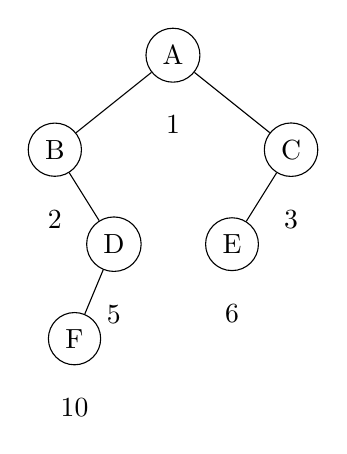
\begin{tikzpicture}[level distance=1.2cm,
level 1/.style={sibling distance=3cm},
level 2/.style={sibling distance=1.5cm},
level 3/.style={sibling distance=1cm}]

\node[circle,draw] (1) {A}
    child {node[circle,draw] (2) {B}
        child[missing]
        child {node[circle,draw] (5) {D}
            child {node[circle,draw] (10) {F}}
            child[missing]}}
    child {node[circle,draw] (3) {C}
        child {node[circle,draw] (6) {E}}
        child[missing]};

% 添加编号
\node[below=0.3cm of 1] {1};
\node[below=0.3cm of 2] {2};
\node[below=0.3cm of 3] {3};
\node[below=0.3cm of 5] {5};
\node[below=0.3cm of 6] {6};
\node[below=0.3cm of 10] {10};
\end{tikzpicture}
\end{center}

顺序存储数组:
\begin{center}
\begin{tabular}{|c|c|c|c|c|c|c|c|c|c|c|}
\hline
下标 & 1 & 2 & 3 & 4 & 5 & 6 & 7 & 8 & 9 & 10 \\
\hline
元素 & A & B & C & $\emptyset$ & D & E & $\emptyset$ & $\emptyset$ & $\emptyset$ & F \\
\hline
\end{tabular}
\end{center}

\subsection{二叉链表}

二叉链表的结点结构:
\begin{center}
\begin{tabular}{|c|c|c|}
\hline
lchild & data & rchild \\
\hline
\end{tabular}
\end{center}

\begin{lstlisting}[caption=二叉链表结点定义]
template <typename DataType>
struct BiNode {
    DataType data;
    BiNode<DataType> *lchild, *rchild;
};
\end{lstlisting}

\section{二叉树的遍历}

\subsection{遍历方法}

二叉树的遍历是指从根结点出发,按照某种次序访问二叉树中的所有结点,使得每个结点被访问一次且仅被访问一次。

\begin{definition}[前序遍历]
若二叉树为空,则空操作返回;否则执行下述操作:
\begin{enumerate}
\item 访问根结点;
\item 前序遍历根结点的左子树;
\item 前序遍历根结点的右子树。
\end{enumerate}
\end{definition}

\begin{definition}[中序遍历]
若二叉树为空,则空操作返回;否则执行下述操作:
\begin{enumerate}
\item 中序遍历根结点的左子树;
\item 访问根结点;
\item 中序遍历根结点的右子树。
\end{enumerate}
\end{definition}

\begin{definition}[后序遍历]
若二叉树为空,则空操作返回;否则执行下述操作:
\begin{enumerate}
\item 后序遍历根结点的左子树;
\item 后序遍历根结点的右子树;
\item 访问根结点。
\end{enumerate}
\end{definition}

\begin{definition}[层序遍历]
从二叉树的根结点开始,从上至下逐层遍历,同一层按从左到右的顺序对结点逐个访问。
\end{definition}

\subsection{遍历算法实现}

\noindent

\begin{algorithm}[H]
\caption{前序遍历递归算法}
\begin{algorithmic}[1]
\REQUIRE 二叉树根指针$bt$
\ENSURE 输出前序遍历序列
\IF{$bt \neq NULL$}
\STATE 访问$bt$的数据域
\STATE 前序遍历$bt$的左子树
\STATE 前序遍历$bt$的右子树
\ENDIF
\end{algorithmic}
\end{algorithm}

\begin{lstlisting}[caption=前序遍历递归实现]
template <typename DataType>
void PreOrder(BiNode<DataType> *bt) {
    if (bt == nullptr) return;
    cout << bt->data << "\t";    // 访问根结点
    PreOrder(bt->lchild);        // 遍历左子树
    PreOrder(bt->rchild);        // 遍历右子树
}
\end{lstlisting}

\begin{example}[前序遍历示例]
给定如下二叉树:
\begin{center}
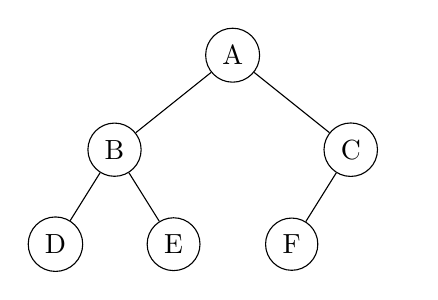
\begin{tikzpicture}[level distance=1.2cm,
    level 1/.style={sibling distance=3cm},
    level 2/.style={sibling distance=1.5cm},
    level 3/.style={sibling distance=1cm}]
\node[circle,draw] {A}
    child {node[circle,draw] {B}
        child {node[circle,draw] {D}}
        child {node[circle,draw] {E}}
    }
    child {node[circle,draw] {C}
        child {node[circle,draw] {F}}
        child {edge from parent[draw=none]}
    };
\end{tikzpicture}
\end{center}

前序遍历过程:
\begin{enumerate}
\item 访问根结点A,输出A
\item 前序遍历左子树(以B为根):
    \begin{itemize}
    \item 访问B,输出B
    \item 前序遍历B的左子树:访问D,输出D
    \item 前序遍历B的右子树:访问E,输出E
    \end{itemize}
\item 前序遍历右子树(以C为根):
    \begin{itemize}
    \item 访问C,输出C
    \item 前序遍历C的左子树:访问F,输出F
    \item 前序遍历C的右子树:空
    \end{itemize}
\end{enumerate}

\textbf{前序遍历结果:A B D E C F}
\end{example}

\begin{algorithm}[H]
\caption{中序遍历递归算法}
\begin{algorithmic}[1]
\REQUIRE 二叉树根指针$bt$
\ENSURE 输出中序遍历序列
\IF{$bt \neq NULL$}
\STATE 中序遍历$bt$的左子树
\STATE 访问$bt$的数据域
\STATE 中序遍历$bt$的右子树
\ENDIF
\end{algorithmic}
\end{algorithm}

\begin{lstlisting}[caption=中序遍历递归实现]
template <typename DataType>
void InOrder(BiNode<DataType> *bt) {
    if (bt == nullptr) return;
    InOrder(bt->lchild);         // 遍历左子树
    cout << bt->data << "\t";    // 访问根结点
    InOrder(bt->rchild);         // 遍历右子树
}
\end{lstlisting}
\begin{center}
    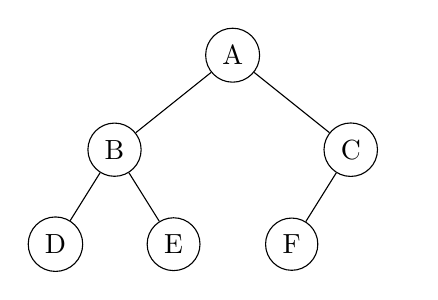
\begin{tikzpicture}[level distance=1.2cm,
        level 1/.style={sibling distance=3cm},
        level 2/.style={sibling distance=1.5cm},
        level 3/.style={sibling distance=1cm}]
    \node[circle,draw] {A}
        child {node[circle,draw] {B}
            child {node[circle,draw] {D}}
            child {node[circle,draw] {E}}
        }
        child {node[circle,draw] {C}
            child {node[circle,draw] {F}}
            child {edge from parent[draw=none]}
        };
    \end{tikzpicture}
    \end{center}
\begin{example}[中序遍历示例]
使用同一棵二叉树,中序遍历过程:
\begin{enumerate}
\item 中序遍历左子树(以B为根):
    \begin{itemize}
    \item 中序遍历B的左子树:访问D,输出D
    \item 访问B,输出B
    \item 中序遍历B的右子树:访问E,输出E
    \end{itemize}
\item 访问根结点A,输出A
\item 中序遍历右子树(以C为根):
    \begin{itemize}
    \item 中序遍历C的左子树:访问F,输出F
    \item 访问C,输出C
    \item 中序遍历C的右子树:空
    \end{itemize}
\end{enumerate}

\textbf{中序遍历结果:D B E A F C}
\end{example}

\begin{algorithm}[H]
\caption{后序遍历递归算法}
\begin{algorithmic}[1]
\REQUIRE 二叉树根指针$bt$
\ENSURE 输出后序遍历序列
\IF{$bt \neq NULL$}
\STATE 后序遍历$bt$的左子树
\STATE 后序遍历$bt$的右子树
\STATE 访问$bt$的数据域
\ENDIF
\end{algorithmic}
\end{algorithm}

\begin{lstlisting}[caption=后序遍历递归实现]
template <typename DataType>
void PostOrder(BiNode<DataType> *bt) {
    if (bt == nullptr) return;
    PostOrder(bt->lchild);       // 遍历左子树
    PostOrder(bt->rchild);       // 遍历右子树
    cout << bt->data << "\t";    // 访问根结点
}
\end{lstlisting}
\begin{center}
    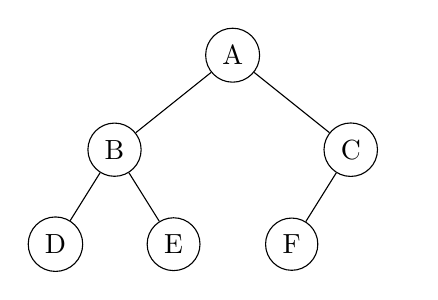
\begin{tikzpicture}[level distance=1.2cm,
        level 1/.style={sibling distance=3cm},
        level 2/.style={sibling distance=1.5cm},
        level 3/.style={sibling distance=1cm}]
    \node[circle,draw] {A}
        child {node[circle,draw] {B}
            child {node[circle,draw] {D}}
            child {node[circle,draw] {E}}
        }
        child {node[circle,draw] {C}
            child {node[circle,draw] {F}}
            child {edge from parent[draw=none]}
        };
    \end{tikzpicture}
    \end{center}
\begin{example}[后序遍历示例]
使用同一棵二叉树,后序遍历过程:
\begin{enumerate}
\item 后序遍历左子树(以B为根):
    \begin{itemize}
    \item 后序遍历B的左子树:访问D,输出D
    \item 后序遍历B的右子树:访问E,输出E
    \item 访问B,输出B
    \end{itemize}
\item 后序遍历右子树(以C为根):
    \begin{itemize}
    \item 后序遍历C的左子树:访问F,输出F
    \item 后序遍历C的右子树:空
    \item 访问C,输出C
    \end{itemize}
\item 访问根结点A,输出A
\end{enumerate}

\textbf{后序遍历结果:D E B F C A}
\end{example}

\begin{example}[更复杂的遍历示例]
考虑一个更复杂的二叉树:
\begin{center}
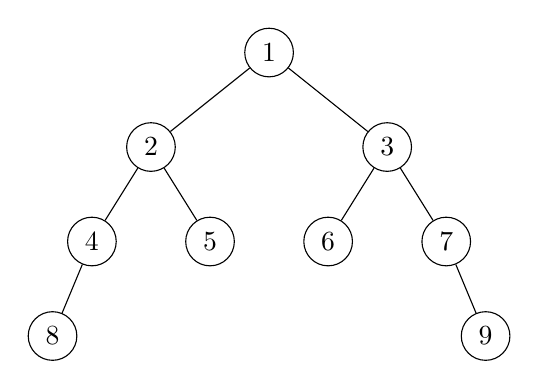
\begin{tikzpicture}[level distance=1.2cm,
    level 1/.style={sibling distance=3cm},
    level 2/.style={sibling distance=1.5cm},
    level 3/.style={sibling distance=1cm}]
\node[circle,draw] {1}
    child {node[circle,draw] {2}
        child {node[circle,draw] {4}
            child {node[circle,draw] {8}}
            child[missing]
        }
        child {node[circle,draw] {5}}
    }
    child {node[circle,draw] {3}
        child {node[circle,draw] {6}}
        child {node[circle,draw] {7}
            child[missing]
            child {node[circle,draw] {9}}
        }
    };
\end{tikzpicture}
\end{center}

\textbf{三种遍历结果比较:}
\begin{itemize}
\item \textbf{前序遍历:}1 2 4 8 5 3 6 7 9
\item \textbf{中序遍历:}8 4 2 5 1 6 3 7 9
\item \textbf{后序遍历:}8 4 5 2 6 9 7 3 1
\end{itemize}

\textbf{规律总结:}
\begin{itemize}
\item 前序遍历:根结点总是在对应子树的最前面
\item 中序遍历:根结点总是在其左右子树之间
\item 后序遍历:根结点总是在对应子树的最后面
\end{itemize}
\end{example}

\subsection{非递归遍历算法}

\indent

\begin{algorithm}[H]
\caption{前序遍历非递归算法}
\begin{algorithmic}[1]
\REQUIRE 二叉树根指针$bt$
\ENSURE 输出前序遍历序列
\STATE 初始化栈$S$
\IF{二叉树非空}
    \STATE 将根指针$bt$入栈
    \WHILE{栈$S$不为空}
        \STATE $p \leftarrow$ 栈顶元素出栈
        \STATE 访问结点$p$的数据域
        \IF{结点$p$存在右孩子}
            \STATE 将右孩子指针入栈
        \ENDIF
        \IF{结点$p$存在左孩子}
            \STATE 将左孩子指针入栈
        \ENDIF
    \ENDWHILE
\ENDIF
\end{algorithmic}
\end{algorithm}

\begin{lstlisting}[caption=前序遍历非递归实现]
template <typename DataType>
void PreOrderNonRecur(BiNode<DataType> *bt) {
    if (bt == nullptr) return;
    stack<BiNode<DataType>*> S;
    S.push(bt);
    
    while (!S.empty()) {
        BiNode<DataType> *p = S.top();
        S.pop();
        cout << p->data << "\t";    // 访问结点
        
        if (p->rchild != nullptr)   // 右孩子先入栈
            S.push(p->rchild);
        if (p->lchild != nullptr)   // 左孩子后入栈(先出栈)
            S.push(p->lchild);
    }
}
\end{lstlisting}

\begin{algorithm}[H]
\caption{中序遍历非递归算法}
\begin{algorithmic}[1]
\REQUIRE 二叉树根指针$bt$
\ENSURE 输出中序遍历序列
\STATE 初始化栈$S$
\STATE $p \leftarrow bt$
\WHILE{$p \neq NULL$ OR 栈$S$不为空}
    \WHILE{$p \neq NULL$}
        \STATE 将$p$入栈
        \STATE $p \leftarrow p$的左孩子
    \ENDWHILE
    \IF{栈$S$不为空}
        \STATE $p \leftarrow$ 栈顶元素出栈
        \STATE 访问结点$p$的数据域
        \STATE $p \leftarrow p$的右孩子
    \ENDIF
\ENDWHILE
\end{algorithmic}
\end{algorithm}

\begin{lstlisting}[caption=中序遍历非递归实现]
template <typename DataType>
void InOrderNonRecur(BiNode<DataType> *bt) {
    stack<BiNode<DataType>*> S;
    BiNode<DataType> *p = bt;
    
    while (p != nullptr || !S.empty()) {
        while (p != nullptr) {      // 一直向左走到底
            S.push(p);
            p = p->lchild;
        }
        if (!S.empty()) {
            p = S.top();
            S.pop();
            cout << p->data << "\t";    // 访问结点
            p = p->rchild;              // 转向右子树
        }
    }
}
\end{lstlisting}

\begin{algorithm}[H]
\caption{后序遍历非递归算法}
\begin{algorithmic}[1]
\REQUIRE 二叉树根指针$bt$
\ENSURE 输出后序遍历序列
\STATE 初始化栈$S$
\STATE $p \leftarrow bt$, $r \leftarrow NULL$
\WHILE{$p \neq NULL$ OR 栈$S$不为空}
    \IF{$p \neq NULL$}
        \STATE 将$p$入栈
        \STATE $p \leftarrow p$的左孩子
    \ELSE
        \STATE $p \leftarrow$ 栈顶元素(不出栈)
        \IF{$p$的右孩子存在且$p$的右孩子$\neq r$}
            \STATE $p \leftarrow p$的右孩子
        \ELSE
            \STATE $p \leftarrow$ 栈顶元素出栈
            \STATE 访问结点$p$的数据域
            \STATE $r \leftarrow p$
            \STATE $p \leftarrow NULL$
        \ENDIF
    \ENDIF
\ENDWHILE
\end{algorithmic}
\end{algorithm}

\begin{lstlisting}[caption=后序遍历非递归实现]
template <typename DataType>
void PostOrderNonRecur(BiNode<DataType> *bt) {
    if (bt == nullptr) return;
    stack<BiNode<DataType>*> S;
    BiNode<DataType> *p = bt;
    BiNode<DataType> *r = nullptr;  // 标记最近访问过的结点
    
    while (p != nullptr || !S.empty()) {
        if (p != nullptr) {         // 走到最左边
            S.push(p);
            p = p->lchild;
        } else {
            p = S.top();            // 查看栈顶元素
            if (p->rchild != nullptr && p->rchild != r) {
                p = p->rchild;      // 转向右子树
            } else {
                p = S.top();
                S.pop();
                cout << p->data << "\t";  // 访问结点
                r = p;              // 记录最近访问的结点
                p = nullptr;        // 结点访问完后,重置p指针
            }
        }
    }
}
\end{lstlisting}

\begin{algorithm}[H]
\caption{层序遍历算法}
\begin{algorithmic}[1]
\REQUIRE 二叉树根指针$bt$
\ENSURE 输出层序遍历序列
\STATE 初始化队列$Q$
\IF{二叉树非空}
    \STATE 将根指针入队
    \WHILE{队列$Q$不为空}
        \STATE $q \leftarrow$ 队头元素出队
        \STATE 访问结点$q$的数据域
        \IF{结点$q$存在左孩子}
            \STATE 将左孩子指针入队
        \ENDIF
        \IF{结点$q$存在右孩子}
            \STATE 将右孩子指针入队
        \ENDIF
    \ENDWHILE
\ENDIF
\end{algorithmic}
\end{algorithm}

\begin{lstlisting}[caption=层序遍历实现]
template <typename DataType>
void LevelOrder(BiNode<DataType> *bt) {
    if (bt == nullptr) return;
    queue<BiNode<DataType>*> Q;
    Q.push(bt);
    
    while (!Q.empty()) {
        BiNode<DataType> *q = Q.front();
        Q.pop();
        cout << q->data << "\t";    // 访问结点
        
        if (q->lchild != nullptr)   // 左孩子入队
            Q.push(q->lchild);
        if (q->rchild != nullptr)   // 右孩子入队
            Q.push(q->rchild);
    }
}
\end{lstlisting}

\subsection{遍历算法复杂度分析}

\begin{theorem}[遍历算法时间复杂度]
对于具有$n$个结点的二叉树:
\begin{itemize}
\item 递归遍历算法的时间复杂度均为$O(n)$,空间复杂度为$O(h)$,其中$h$为树的高度
\item 非递归遍历算法的时间复杂度均为$O(n)$,空间复杂度为$O(h)$
\item 层序遍历算法的时间复杂度为$O(n)$,空间复杂度为$O(w)$,其中$w$为树的最大宽度
\end{itemize}
\end{theorem}

\subsection{遍历示例}

\begin{center}
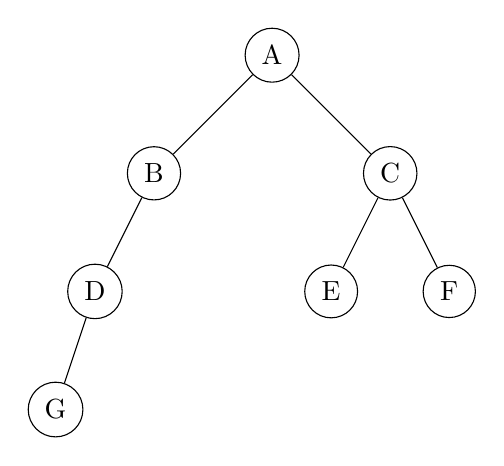
\begin{tikzpicture}[level distance=1.5cm,
level 1/.style={sibling distance=3cm},
level 2/.style={sibling distance=1.5cm},
level 3/.style={sibling distance=1cm}]

\node[circle,draw] {A}
    child {node[circle,draw] {B}
        child {node[circle,draw] {D}
            child {node[circle,draw] {G}}
            child[missing]}
        child[missing]}
    child {node[circle,draw] {C}
        child {node[circle,draw] {E}}
        child {node[circle,draw] {F}}};
\end{tikzpicture}
\end{center}

对于上述二叉树,各种遍历序列为:
\begin{itemize}
\item 前序遍历:A B D G C E F
\item 中序遍历:G D B A E C F
\item 后序遍历:G D B E F C A
\item 层序遍历:A B C D E F G
\end{itemize}

\section{二叉树的构造}

\begin{theorem}
前序遍历序列和中序遍历序列能唯一确定一棵二叉树。
\end{theorem}

\begin{example}[由遍历序列构造二叉树]
已知一棵二叉树的前序遍历序列为ABDCEF,中序遍历序列为DBAECF,构造该二叉树。

\textbf{解:}
\begin{enumerate}
\item 由前序序列可知,A是二叉树的根结点。
\item 根据中序序列,在A之前的所有结点(DB)都是A的左子树的结点,在A之后的所有结点(ECF)都是A的右子树的结点。
\item 对左子树:前序序列为BD,中序序列为DB。由前序序列知B是左子树的根结点,由中序序列知D是B的左子树结点。
\item 对右子树:前序序列为CEF,中序序列为ECF。由前序序列知C是右子树的根结点,由中序序列知E是C的左子树结点,F是C的右子树结点。
\end{enumerate}

构造过程如下:

\begin{center}
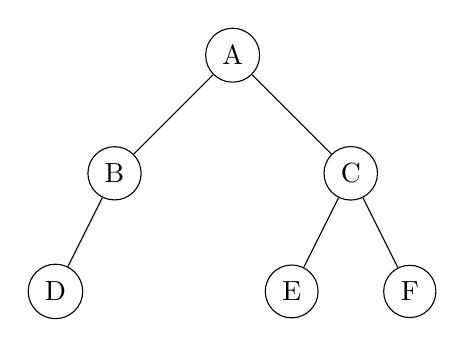
\begin{tikzpicture}[level distance=1.5cm,
level 1/.style={sibling distance=3cm},
level 2/.style={sibling distance=1.5cm}]

\node[circle,draw] {A}
    child {node[circle,draw] {B}
        child {node[circle,draw] {D}}
        child[missing]}
    child {node[circle,draw] {C}
        child {node[circle,draw] {E}}
        child {node[circle,draw] {F}}};
\end{tikzpicture}
\end{center}
\end{example}

\section{线索二叉树}

\subsection{线索二叉树的基本概念}

在具有$n$个结点的二叉链表中,共有$2n$个指针域,其中只有$n-1$个指针域用来存储孩子结点的地址,存在$n+1$个空指针域。可以利用这些空指针指向该结点在某种遍历序列中的前驱和后继结点。

\begin{definition}[线索]
指向前驱和后继结点的指针称为线索。
\end{definition}

\begin{definition}[线索二叉树]
加上线索的二叉树称为线索二叉树。
\end{definition}

\subsection{线索二叉树的结点结构}

\begin{center}
\begin{tabular}{|c|c|c|c|c|}
\hline
lchild & ltag & data & rtag & rchild \\
\hline
\end{tabular}
\end{center}

其中:
$$ltag = \begin{cases}
0 & \text{lchild指向该结点的左孩子} \\
1 & \text{lchild指向该结点的前驱}
\end{cases}$$

$$rtag = \begin{cases}
0 & \text{rchild指向该结点的右孩子} \\
1 & \text{rchild指向该结点的后继}
\end{cases}$$

\begin{lstlisting}[caption=线索二叉树结点定义]
template <typename DataType>
struct ThrNode {
    DataType data;
    int ltag, rtag;
    ThrNode<DataType> *lchild, *rchild;
};
\end{lstlisting}

\section{哈夫曼树}

\subsection{基本概念}

\begin{definition}[权值]
叶子结点的权值是对叶子结点赋予的一个有意义的数值量。
\end{definition}

\begin{definition}[带权路径长度]
设二叉树具有$n$个带权值的叶子结点,从根结点到各个叶子结点的路径长度与相应叶子结点权值的乘积之和称为二叉树的带权路径长度,记为:
$$WPL = \sum_{k=1}^{n} w_k l_k$$
其中,$w_k$为第$k$个叶子结点的权值;$l_k$为从根结点到第$k$个叶子结点的路径长度。
\end{definition}

\begin{definition}[哈夫曼树]
带权路径长度最小的二叉树称为最优二叉树,也称哈夫曼树。
\end{definition}

\subsection{哈夫曼算法}

\begin{algorithm}[H]
\caption{哈夫曼算法}
\begin{algorithmic}[1]
\REQUIRE $n$个权值$\{w_1, w_2, \ldots, w_n\}$
\ENSURE 哈夫曼树
\STATE 初始化:由$\{w_1, w_2, \ldots, w_n\}$构造$n$棵只有一个根结点的二叉树,从而得到一个二叉树集合$F = \{T_1, T_2, \ldots, T_n\}$
\WHILE{集合$F$中的二叉树个数大于1}
    \STATE 选取与合并:在$F$中选取根结点的权值最小的两棵二叉树分别作为左右子树构造一棵新的二叉树,新根结点的权值为其左右子树根结点的权值之和
    \STATE 删除与加入:在$F$中删除作为左右子树的两棵二叉树,并将新建立的二叉树加入到$F$中
\ENDWHILE
\end{algorithmic}
\end{algorithm}

\begin{example}[哈夫曼树构造]
给定权值集合$\{2, 3, 4, 5\}$,构造哈夫曼树。

\textbf{解:}

\begin{center}
\textbf{构造步骤:}

\begin{enumerate}
\item \textbf{初始状态:}四个独立结点,权值分别为2, 3, 4, 5
\item \textbf{第一步:}选择权值最小的两个结点(2和3)进行合并,生成权值为5的新结点
\item \textbf{第二步:}选择权值最小的两个结点(4和5)进行合并,生成权值为9的新结点
\item \textbf{第三步:}最后将两个子树(权值为5和9)合并,生成根结点,权值为14
\end{enumerate}

\textbf{步骤1:初始状态}

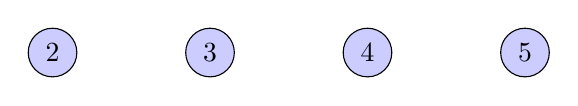
\begin{tikzpicture}
\node[circle,draw,fill=blue!20] at (0,0) {2};
\node[circle,draw,fill=blue!20] at (2,0) {3};
\node[circle,draw,fill=blue!20] at (4,0) {4};
\node[circle,draw,fill=blue!20] at (6,0) {5};
\end{tikzpicture}

\vspace{0.8cm}

\textbf{步骤2:第一次合并(2 + 3 = 5)}

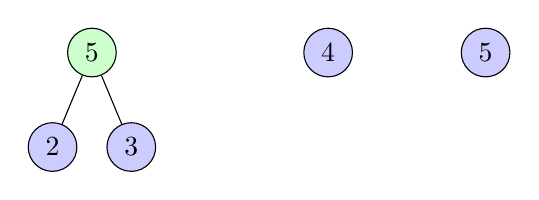
\begin{tikzpicture}[level distance=1.2cm, sibling distance=1cm]
\node[circle,draw,fill=green!20] at (1,0) {5}
    child {node[circle,draw,fill=blue!20] {2}}
    child {node[circle,draw,fill=blue!20] {3}};
\node[circle,draw,fill=blue!20] at (4,0) {4};
\node[circle,draw,fill=blue!20] at (6,0) {5};
\end{tikzpicture}

\vspace{0.8cm}

\textbf{步骤3:第二次合并(4 + 5 = 9)}

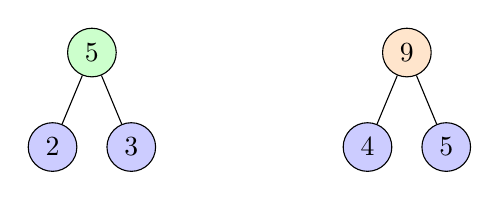
\begin{tikzpicture}[level distance=1.2cm, sibling distance=1cm]
\node[circle,draw,fill=green!20] at (1,0) {5}
    child {node[circle,draw,fill=blue!20] {2}}
    child {node[circle,draw,fill=blue!20] {3}};
\node[circle,draw,fill=orange!20] at (5,0) {9}
    child {node[circle,draw,fill=blue!20] {4}}
    child {node[circle,draw,fill=blue!20] {5}};
\end{tikzpicture}

\vspace{0.8cm}

\textbf{步骤4:最终合并(5 + 9 = 14)}

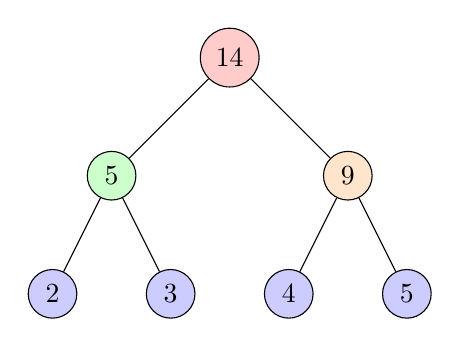
\begin{tikzpicture}[level distance=1.5cm, 
level 1/.style={sibling distance=3cm},
level 2/.style={sibling distance=1.5cm}]
\node[circle,draw,fill=red!20] {14}
    child {node[circle,draw,fill=green!20] {5}
        child {node[circle,draw,fill=blue!20] {2}}
        child {node[circle,draw,fill=blue!20] {3}}}
    child {node[circle,draw,fill=orange!20] {9}
        child {node[circle,draw,fill=blue!20] {4}}
        child {node[circle,draw,fill=blue!20] {5}}};
\end{tikzpicture}
\end{center}
该哈夫曼树的带权路径长度计算如下:

根据带权路径长度公式 $WPL = \sum_{k=1}^{n} w_k l_k$,我们需要计算每个叶子结点的权值乘以其到根结点的路径长度:

\begin{itemize}
\item 权值为2的叶子结点:从根结点到该结点需要经过3条边(根→左子树→左子树→左叶子),所以路径长度$l_1 = 3$
\item 权值为3的叶子结点:从根结点到该结点需要经过3条边(根→左子树→左子树→右叶子),所以路径长度$l_2 = 3$  
\item 权值为4的叶子结点:从根结点到该结点需要经过2条边(根→右子树→左叶子),所以路径长度$l_3 = 2$
\item 权值为5的叶子结点:从根结点到该结点需要经过2条边(根→右子树→右叶子),所以路径长度$l_4 = 2$
\end{itemize}

因此,带权路径长度为:
$$WPL = 2 \times 3 + 3 \times 3 + 4 \times 2 + 5 \times 2 = 6 + 9 + 8 + 10 = 33$$
\end{example}

\subsection{哈夫曼编码}

哈夫曼树可用于构造最短的不等长编码方案:
\begin{enumerate}
\item 以字符作为叶子结点,频率作为权值构造哈夫曼树
\item 规定左分支代表0,右分支代表1
\item 从根结点到叶子结点的路径组成该字符的编码
\end{enumerate}

\begin{example}[哈夫曼编码]
字符集$\{A, B, C, D, E\}$,使用频率分别为$\{35, 25, 15, 15, 10\}$,构造哈夫曼编码。

\textbf{构造步骤:}

\textbf{步骤1:}将所有字符按频率从小到大排列:$E(10), C(15), D(15), B(25), A(35)$

\textbf{步骤2:}选择频率最小的两个结点$E(10)$和$C(15)$合并,得到新结点权值为$10+15=25$

\textbf{步骤3:}选择频率最小的两个结点$D(15)$和新结点$(25)$合并,得到新结点权值为$15+25=40$

\textbf{步骤4:}选择频率最小的两个结点$B(25)$和$A(35)$合并,得到新结点权值为$25+35=60$

\textbf{步骤5:}最后合并剩余的两个结点$(40)$和$(60)$,得到根结点权值为$40+60=100$

\begin{center}
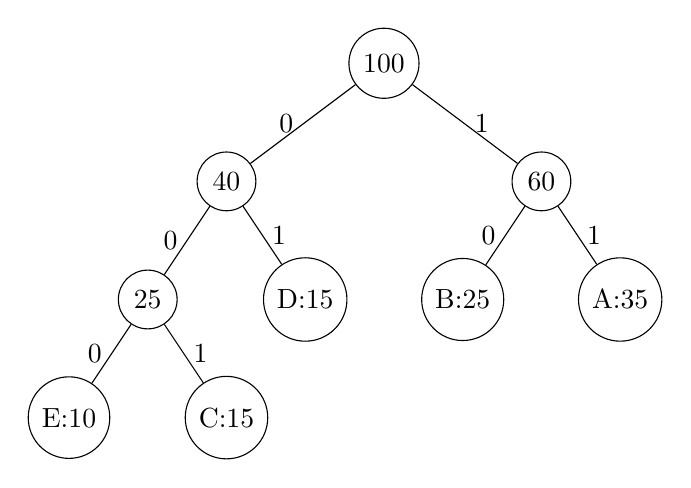
\begin{tikzpicture}[level distance=1.5cm,
level 1/.style={sibling distance=4cm},
level 2/.style={sibling distance=2cm},
level 3/.style={sibling distance=2cm}]

\node[circle,draw] {100}
    child {node[circle,draw] {40}
        child {node[circle,draw] {25}
            child {node[circle,draw] {E:10}
                edge from parent node[left] {0}}
            child {node[circle,draw] {C:15}
                edge from parent node[right] {1}}
            edge from parent node[left] {0}}
        child {node[circle,draw] {D:15}
            edge from parent node[right] {1}}
        edge from parent node[left] {0}}
    child {node[circle,draw] {60}
        child {node[circle,draw] {B:25}
            edge from parent node[left] {0}}
        child {node[circle,draw] {A:35}
            edge from parent node[right] {1}}
        edge from parent node[right] {1}};
\end{tikzpicture}
\end{center}

\textbf{编码方法:}
\begin{enumerate}
\item 规定左分支代表0,右分支代表1
\item 从根结点到每个叶子结点的路径组成该字符的编码
\item 具体编码过程:
\begin{itemize}
\item 字符A:根→右→右,编码为11
\item 字符B:根→右→左,编码为10
\item 字符C:根→左→左→右,编码为001
\item 字符D:根→左→右,编码为01
\item 字符E:根→左→左→左,编码为000
\end{itemize}
\end{enumerate}

编码结果:
\begin{center}
\begin{tabular}{|c|c|c|c|}
\hline
字符 & 频率 & 编码 & 编码长度 \\
\hline
A & 35 & 11 & 2 \\
B & 25 & 10 & 2 \\
C & 15 & 001 & 3 \\
D & 15 & 01 & 2 \\
E & 10 & 000 & 3 \\
\hline
\end{tabular}
\end{center}

\textbf{编码特点:}
\begin{itemize}
\item 频率高的字符使用较短的编码(A、B、D使用2位编码)
\item 频率低的字符使用较长的编码(C、E使用3位编码)
\item 任何字符的编码都不是另一个字符编码的前缀(前缀码性质)
\end{itemize}
\end{example}

\section{堆与优先队列}

\subsection{堆的定义与性质}

\begin{definition}[堆]
堆是具有下列性质的完全二叉树:
\begin{itemize}
\item \textbf{大根堆(最大堆)}:每个结点的值都大于或等于其左右孩子结点的值
\item \textbf{小根堆(最小堆)}:每个结点的值都小于或等于其左右孩子结点的值
\end{itemize}
\end{definition}

\textbf{堆的重要性质:}
\begin{enumerate}
\item 堆是完全二叉树,可以用数组存储,节省空间
\item 如果将堆按层序从1开始编号,则结点之间满足如下关系:
$$\text{大根堆:}\begin{cases}
k_i \geq k_{2i} \\
k_i \geq k_{2i+1}
\end{cases} \quad \text{小根堆:}\begin{cases}
k_i \leq k_{2i} \\
k_i \leq k_{2i+1}
\end{cases} \quad (1 \leq i \leq \lfloor n/2 \rfloor)$$
\item 对于编号为$i$的结点:
\begin{itemize}
\item 父结点编号:$\lfloor i/2 \rfloor$
\item 左孩子编号:$2i$
\item 右孩子编号:$2i+1$
\end{itemize}
\end{enumerate}

\textbf{堆的示例:}
\begin{center}
\begin{tikzpicture}[level distance=1.5cm,
level 1/.style={sibling distance=3cm},
level 2/.style={sibling distance=1.5cm},
level 3/.style={sibling distance=1cm}]

\node[circle,draw] {90}
    child {node[circle,draw] {80}
        child {node[circle,draw] {65}}
        child {node[circle,draw] {70}}}
    child {node[circle,draw] {85}
        child {node[circle,draw] {60}}
        child {node[circle,draw] {75}}};

\node at (0,-4) {\textbf{大根堆示例}};
\end{tikzpicture}
\quad
\begin{tikzpicture}[level distance=1.5cm,
level 1/.style={sibling distance=3cm},
level 2/.style={sibling distance=1.5cm},
level 3/.style={sibling distance=1cm}]

\node[circle,draw] {10}
    child {node[circle,draw] {20}
        child {node[circle,draw] {35}}
        child {node[circle,draw] {30}}}
    child {node[circle,draw] {15}
        child {node[circle,draw] {40}}
        child {node[circle,draw] {25}}};

\node at (0,-4) {\textbf{小根堆示例}};
\end{tikzpicture}
\end{center}

\subsection{堆的基本操作}

\subsubsection{堆的插入操作(向上调整)}

\textbf{算法思想:}
\begin{enumerate}
\item 将新元素插入到堆的末尾(保持完全二叉树性质)
\item 将新元素与其父结点比较,如果违反堆的性质则交换
\item 重复步骤2,直到满足堆的性质或到达根结点
\end{enumerate}

\begin{algorithm}[H]
\caption{堆的插入操作(大根堆)}
\begin{algorithmic}[1]
\REQUIRE 待插入元素$x$,堆数组$heap[]$,堆大小$size$
\ENSURE 维护堆的性质
\STATE $size \leftarrow size + 1$
\STATE $heap[size] \leftarrow x$
\STATE $i \leftarrow size$
\WHILE{$i > 1$ 且 $heap[i] > heap[i/2]$}
    \STATE 交换$heap[i]$和$heap[i/2]$
    \STATE $i \leftarrow i/2$
\ENDWHILE
\end{algorithmic}
\end{algorithm}

\begin{lstlisting}[caption=堆插入操作的C++实现]
void insertHeap(vector<int>& heap, int x) {
    heap.push_back(x);
    int i = heap.size() - 1;
    
    // 向上调整
    while (i > 0 && heap[i] > heap[(i-1)/2]) {
        swap(heap[i], heap[(i-1)/2]);
        i = (i-1)/2;
    }
}
\end{lstlisting}

\subsubsection{堆的删除操作(向下调整)}

\textbf{算法思想:}
\begin{enumerate}
\item 保存堆顶元素(要删除的元素)
\item 将堆的最后一个元素移到堆顶
\item 从堆顶开始向下调整,与较大的孩子交换(大根堆)
\item 重复调整直到满足堆的性质
\end{enumerate}

\begin{algorithm}[H]
\caption{堆的删除操作(大根堆)}
\begin{algorithmic}[1]
\REQUIRE 堆数组$heap[]$,堆大小$size$
\ENSURE 删除堆顶元素并维护堆的性质
\STATE $result \leftarrow heap[1]$
\STATE $heap[1] \leftarrow heap[size]$
\STATE $size \leftarrow size - 1$
\STATE $i \leftarrow 1$
\WHILE{$2i \leq size$}
    \STATE $j \leftarrow 2i$ \COMMENT{左孩子}
    \IF{$j < size$ 且 $heap[j] < heap[j+1]$}
        \STATE $j \leftarrow j+1$ \COMMENT{选择较大的孩子}
    \ENDIF
    \IF{$heap[i] \geq heap[j]$}
        \STATE \textbf{break} \COMMENT{已满足堆性质}
    \ELSE
        \STATE 交换$heap[i]$和$heap[j]$
        \STATE $i \leftarrow j$
    \ENDIF
\ENDWHILE
\RETURN $result$
\end{algorithmic}
\end{algorithm}

\subsubsection{建堆操作}

\textbf{方法一:逐个插入法}
\begin{itemize}
\item 从空堆开始,逐个插入元素
\item 时间复杂度:$O(n \log n)$
\end{itemize}

\textbf{方法二:自底向上调整法(更高效)}
\begin{itemize}
\item 将数组看作完全二叉树
\item 从最后一个非叶子结点开始,向前逐个进行向下调整
\item 时间复杂度:$O(n)$
\end{itemize}

\begin{algorithm}[H]
\caption{建堆操作(自底向上)}
\begin{algorithmic}[1]
\REQUIRE 数组$A[1..n]$
\ENSURE 将数组调整为大根堆
\FOR{$i = \lfloor n/2 \rfloor$ \textbf{downto} $1$}
    \STATE 对以$A[i]$为根的子树进行向下调整
\ENDFOR
\end{algorithmic}
\end{algorithm}

\subsection{堆排序}

\textbf{基本思想:}
\begin{enumerate}
\item 将待排序数组建成大根堆
\item 将堆顶元素(最大值)与堆的最后一个元素交换
\item 堆大小减1,对新的堆顶进行向下调整
\item 重复步骤2-3,直到堆大小为1
\end{enumerate}

\begin{lstlisting}[caption=堆排序算法实现]
void heapSort(vector<int>& arr) {
    int n = arr.size();
    
    // 建堆
    for (int i = n/2 - 1; i >= 0; i--) {
        heapify(arr, n, i);
    }
    
    // 排序
    for (int i = n-1; i > 0; i--) {
        swap(arr[0], arr[i]);  // 将最大元素放到末尾
        heapify(arr, i, 0);    // 调整剩余元素
    }
}

void heapify(vector<int>& arr, int n, int i) {
    int largest = i;
    int left = 2*i + 1;
    int right = 2*i + 2;
    
    if (left < n && arr[left] > arr[largest])
        largest = left;
    if (right < n && arr[right] > arr[largest])
        largest = right;
        
    if (largest != i) {
        swap(arr[i], arr[largest]);
        heapify(arr, n, largest);
    }
}
\end{lstlisting}

\textbf{堆排序的特点:}
\begin{itemize}
\item 时间复杂度:$O(n \log n)$(最好、平均、最坏情况都相同)
\item 空间复杂度:$O(1)$(原地排序)
\item 不稳定排序
\item 适合处理大数据量的排序问题
\end{itemize}

\subsection{优先队列}

\begin{definition}[优先队列]
优先队列是一种抽象数据类型,支持以下操作:
\begin{itemize}
\item 插入元素(insert)
\item 删除并返回优先级最高的元素(deleteMax/deleteMin)
\item 查看优先级最高的元素(top/peek)
\end{itemize}
\end{definition}

\textbf{优先队列的实现方式比较:}
\begin{center}
\begin{tabular}{|l|c|c|c|}
\hline
\textbf{实现方式} & \textbf{插入} & \textbf{删除最值} & \textbf{查找最值} \\
\hline
无序数组 & $O(1)$ & $O(n)$ & $O(n)$ \\
\hline
有序数组 & $O(n)$ & $O(1)$ & $O(1)$ \\
\hline
无序链表 & $O(1)$ & $O(n)$ & $O(n)$ \\
\hline
有序链表 & $O(n)$ & $O(1)$ & $O(1)$ \\
\hline
二叉堆 & $O(\log n)$ & $O(\log n)$ & $O(1)$ \\
\hline
\end{tabular}
\end{center}

\textbf{应用实例:}
\begin{enumerate}
\item \textbf{任务调度}:操作系统中根据优先级调度进程
\item \textbf{哈夫曼编码}:构造哈夫曼树时需要反复取出频率最小的结点
\item \textbf{图算法}:Dijkstra最短路径算法、Prim最小生成树算法
\item \textbf{事件模拟}:按时间顺序处理事件
\end{enumerate}

\begin{example}[堆操作过程演示]
对序列$(10, 20, 15, 30, 40)$建立大根堆,然后依次删除堆顶元素。

\textbf{建堆过程:}
\begin{enumerate}
\item 初始数组:$[10, 20, 15, 30, 40]$
\item 从最后一个非叶子结点开始调整($i = \lfloor 5/2 \rfloor = 2$)
\item 调整结点2(值为15):与孩子40比较,交换得到$[10, 20, 40, 30, 15]$
\item 调整结点1(值为20):与孩子30比较,交换得到$[10, 30, 40, 20, 15]$
\item 调整结点0(值为10):与孩子40比较,交换得到$[40, 30, 10, 20, 15]$
\item 继续调整:10与20比较,交换得到$[40, 30, 20, 10, 15]$
\end{enumerate}

\textbf{删除过程:}
\begin{enumerate}
\item 删除40:将15移到堆顶,调整得到$[30, 15, 20, 10]$
\item 删除30:将10移到堆顶,调整得到$[20, 15, 10]$
\item 删除20:将10移到堆顶,调整得到$[15, 10]$
\item 删除15:得到$[10]$
\item 删除10:堆为空
\end{enumerate}
\end{example}

\section{二叉树的应用}

\subsection{表达式树}

二叉表达式树是对应一个算术表达式的二叉树,具有以下特点:
\begin{enumerate}
\item 叶子结点一定是操作数
\item 分支结点一定是运算符
\end{enumerate}

\begin{example}[构造表达式树]
将表达式$(A+B) \times (C+D \times E)$转换为二叉表达式树。

\begin{center}
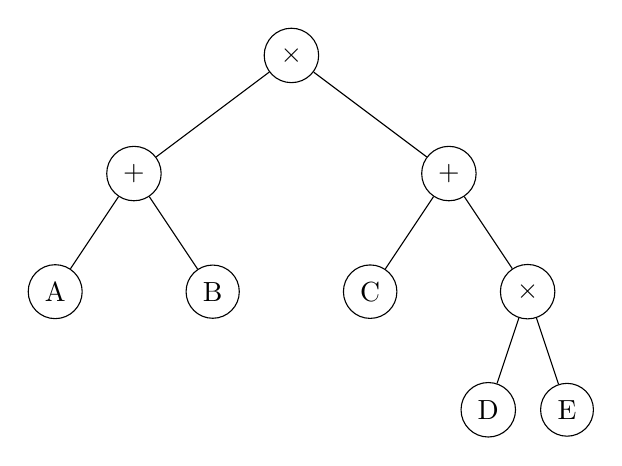
\begin{tikzpicture}[level distance=1.5cm,
level 1/.style={sibling distance=4cm},
level 2/.style={sibling distance=2cm},
level 3/.style={sibling distance=1cm}]

\node[circle,draw] {$\times$}
    child {node[circle,draw] {$+$}
        child {node[circle,draw] {A}}
        child {node[circle,draw] {B}}}
    child {node[circle,draw] {$+$}
        child {node[circle,draw] {C}}
        child {node[circle,draw] {$\times$}
            child {node[circle,draw] {D}}
            child {node[circle,draw] {E}}}};
\end{tikzpicture}
\end{center}

遍历结果:
\begin{itemize}
\item 前序遍历:$\times + A B + C \times D E$(前缀表达式)
\item 中序遍历:$A + B \times C + D \times E$(中缀表达式)
\item 后序遍历:$A B + C D E \times + \times$(后缀表达式)
\end{itemize}
\end{example}

\section{常见考点总结}

\subsection{重点掌握内容}

\begin{enumerate}
\item \textbf{二叉树的基本性质}:特别是性质1($n_0 = n_2 + 1$)和性质5(完全二叉树的编号关系)
\item \textbf{二叉树的遍历}:四种遍历方法的递归和非递归实现
\item \textbf{由遍历序列构造二叉树}:前序+中序或后序+中序唯一确定二叉树
\item \textbf{哈夫曼树的构造和编码}:算法过程和编码方法
\item \textbf{线索二叉树}:线索化过程和在线索二叉树上的遍历
\item \textbf{堆的基本操作}:插入和删除操作的调整过程
\end{enumerate}

\subsection{常见题型}

\begin{enumerate}
\item 根据二叉树的性质计算结点个数、深度等
\item 写出给定二叉树的各种遍历序列
\item 根据遍历序列构造二叉树
\item 设计二叉树遍历的递归和非递归算法
\item 哈夫曼树的构造和编码设计
\item 完全二叉树的性质和应用
\item 线索二叉树的构造和遍历
\end{enumerate}

\subsection{重要算法复杂度}

\begin{center}
\begin{tabular}{|l|c|c|}
\hline
\textbf{操作} & \textbf{时间复杂度} & \textbf{空间复杂度} \\
\hline
二叉树遍历(递归) & $O(n)$ & $O(h)$ \\
二叉树遍历(非递归) & $O(n)$ & $O(h)$ \\
哈夫曼树构造 & $O(n\log n)$ & $O(n)$ \\
堆的插入 & $O(\log n)$ & $O(1)$ \\
堆的删除 & $O(\log n)$ & $O(1)$ \\
线索化 & $O(n)$ & $O(h)$ \\
\hline
\end{tabular}
\end{center}

\section{典型例题解析}

\begin{example}[结点个数计算]
一棵完全二叉树有780个结点,其中叶子结点的个数是多少?

\textbf{解:}
设度为0、1、2的结点个数分别为$n_0$、$n_1$、$n_2$。

由二叉树性质1:$n_0 = n_2 + 1$

总结点数:$n_0 + n_1 + n_2 = 780$

对于完全二叉树,$n_1 \leq 1$(最多只有一个度为1的结点)

代入得:$(n_2 + 1) + n_1 + n_2 = 780$

即:$2n_2 + n_1 + 1 = 780$

所以:$2n_2 + n_1 = 779$

由于$n_1 \leq 1$,当$n_1 = 1$时,$n_2 = 389$,$n_0 = 390$
当$n_1 = 0$时,$n_2 = 389.5$(不是整数,不合理)

因此,叶子结点个数为390。
\end{example}

\begin{example}[遍历序列应用]
已知二叉树的前序遍历序列为ABDHECFIG,中序遍历序列为HDBECAIFG,画出该二叉树。

\textbf{解:}
\begin{enumerate}
\item 由前序序列知A是根结点
\item 由中序序列知,A左边的HDBEC是左子树,A右边的IFG是右子树
\item 递归处理左子树:前序为BDHEC,中序为HDBEC
\item 递归处理右子树:前序为FIG,中序为IFG
\end{enumerate}

最终构造的二叉树如下:

\begin{center}
\begin{tikzpicture}[level distance=1.5cm,
level 1/.style={sibling distance=5cm},
level 2/.style={sibling distance=2.5cm},
level 3/.style={sibling distance=1.5cm}]

\node[circle,draw] {A}
    child {node[circle,draw] {B}
        child {node[circle,draw] {D}
            child {node[circle,draw] {H}}
            child[missing]}
        child {node[circle,draw] {E}
            child[missing]
            child {node[circle,draw] {C}}}}
    child {node[circle,draw] {F}
        child {node[circle,draw] {I}}
        child {node[circle,draw] {G}}};
\end{tikzpicture}
\end{center}
\end{example}

\section{复习建议}

\subsection{学习方法}

\begin{enumerate}
\item \textbf{理解概念}:深入理解二叉树的定义和性质,特别是与普通树的区别
\item \textbf{掌握算法}:熟练掌握各种遍历算法的递归和非递归实现
\item \textbf{练习构造}:通过遍历序列构造二叉树的方法要反复练习
\item \textbf{应用实践}:理解二叉树在实际问题中的应用,如表达式树、哈夫曼编码等
\item \textbf{代码实现}:能够用代码实现二叉树的基本操作
\end{enumerate}

\subsection{复习重点}

\begin{enumerate}
\item 二叉树的五个基本性质及其证明和应用
\item 四种遍历方法的定义、实现和应用
\item 线索二叉树的构造和遍历
\item 哈夫曼树的构造算法和编码方法
\item 堆的定义、性质和基本操作
\item 完全二叉树的性质和应用
\end{enumerate}

\subsection{常见错误}

\begin{enumerate}
\item 混淆二叉树和度为2的树的概念
\item 遍历算法的递归出口条件错误
\item 完全二叉树性质应用错误
\item 哈夫曼编码的构造过程错误
\item 线索二叉树的线索方向搞错
\end{enumerate}

\end{document}
\part{图论}
\documentclass[12pt,a4paper]{amsart}
\usepackage[utf8]{inputenc}
\usepackage[T1]{fontenc}
\usepackage{amsmath,amsfonts,amssymb}
\usepackage{tikz}
\usepackage{algorithm}
\usepackage{algorithmic}
\usepackage{listings}
\usepackage{xcolor}
\usepackage{geometry}
\usepackage{fancyhdr}
\usepackage{enumitem}
\usepackage{booktabs}
\usepackage{multirow}
\usepackage[hidelinks,bookmarksnumbered,bookmarksopen]{hyperref}
\usepackage{xeCJK}
\setCJKmainfont{LXGW WenKai}


% 页面设置
\geometry{left=2cm,right=2cm,top=2.5cm,bottom=2.5cm}
\pagestyle{fancy}
\fancyhf{}
\fancyhead[L]{图论复习总结}
\fancyhead[R]{\thepage}

% TikZ库
\usetikzlibrary{arrows,positioning,shapes,calc,trees,graphs}

% 代码高亮设置
\lstset{
    language=C++,
    basicstyle=\ttfamily\small,
    keywordstyle=\color{blue}\bfseries,
    commentstyle=\color{green!60!black},
    stringstyle=\color{red},
    numbers=left,
    numberstyle=\tiny\color{gray},
    stepnumber=1,
    numbersep=10pt,
    backgroundcolor=\color{gray!10},
    frame=single,
    tabsize=4,
    captionpos=b,
    breaklines=true,
    breakatwhitespace=false,
    showspaces=false,
    showstringspaces=false,
    showtabs=false
}

% 定理环境
\newtheorem{definition}{定义}[section]
\newtheorem{theorem}{定理}[section]
\newtheorem{algorithm_desc}{算法}[section]

\title{\textbf{数据结构第六章:图论复习总结}}
\author{期末考试复习资料}
\date{\today}

\begin{document}

% \maketitle

% % 目录设置
% \tableofcontents
% \newpage

\section{图的基本概念}

\subsection{图的定义}

\begin{definition}[图]
图是由顶点的有穷非空集合和顶点之间边的集合组成,通常表示为:
$$G = (V, E)$$
其中$G$表示一个图,$V$是顶点集合,$E$是边集合。
\end{definition}

\begin{center}
\begin{tikzpicture}[scale=1.2]
    % 无向图示例
    \node[circle,draw,minimum size=0.8cm] (v0) at (0,0) {$v_0$};
    \node[circle,draw,minimum size=0.8cm] (v1) at (2,1) {$v_1$};
    \node[circle,draw,minimum size=0.8cm] (v2) at (2,-1) {$v_2$};
    \node[circle,draw,minimum size=0.8cm] (v3) at (4,0) {$v_3$};
    
    \draw (v0) -- (v1);
    \draw (v0) -- (v2);
    \draw (v1) -- (v3);
    \draw (v2) -- (v3);
    \draw (v1) -- (v2);
    
    \node at (2,-2) {\textbf{无向图}};
    
    % 有向图示例
    \begin{scope}[xshift=6cm]
        \node[circle,draw,minimum size=0.8cm] (u0) at (0,0) {$u_0$};
        \node[circle,draw,minimum size=0.8cm] (u1) at (2,1) {$u_1$};
        \node[circle,draw,minimum size=0.8cm] (u2) at (2,-1) {$u_2$};
        \node[circle,draw,minimum size=0.8cm] (u3) at (4,0) {$u_3$};
        
        \draw[-latex] (u0) -- (u1);
        \draw[-latex] (u0) -- (u2);
        \draw[-latex] (u1) -- (u3);
        \draw[-latex] (u2) -- (u3);
        \draw[-latex,bend left] (u1) to (u2);
        
        \node at (2,-2) {\textbf{有向图}};
    \end{scope}
\end{tikzpicture}
\end{center}

\subsection{图的基本术语}

\begin{itemize}
    \item \textbf{邻接}:若存在边$(v_i, v_j)$,则称$v_i$和$v_j$互为邻接点
    \item \textbf{关联(依附)}:顶点$v$和边$e$相关联,称边$e$依附于顶点$v$
    \item \textbf{度}:
    \begin{itemize}
        \item 无向图:顶点$v$的度$TD(v)$是依附于该顶点的边数
        \item 有向图:入度$ID(v)$ + 出度$OD(v)$
        \item 悬挂顶点:度为1的顶点
        \item 孤立顶点:度为0的顶点
    \end{itemize}
    \item \textbf{路径与回路}:
    \begin{itemize}
        \item 路径:顶点序列$v_p = v_{i_0}v_{i_1}\cdots v_{i_m} = v_q$
        \item 路径长度:路径上边的数目
        \item 简单路径:顶点不重复的路径
        \item 回路(环):第一个和最后一个顶点相同的路径
        \item 简单回路:除第一个和最后一个顶点外,其余顶点不重复的回路
    \end{itemize}
    \item \textbf{连通性}:
    \begin{itemize}
        \item 连通:任意两顶点间都有路径的无向图
        \item 连通分量:无向图中的极大连通子图
        \item 强连通:任意两顶点间都有路径的有向图
        \item 强连通分量:有向图中的极大强连通子图
    \end{itemize}
    \item \textbf{特殊图类型}:
    \begin{itemize}
        \item 完全图:任意两个顶点之间都有边的简单图
        \item 无向完全图:$n$个顶点的完全图有$\frac{n(n-1)}{2}$条边
        \item 有向完全图:$n$个顶点的完全图有$n(n-1)$条弧
        \item 树:$n$个顶点$n-1$条边的连通无向图
        \item 森林:若干棵不相交树的集合
    \end{itemize}
\end{itemize}

\subsection{重要数学性质}

\begin{theorem}[握手定理]
在具有$n$个顶点$e$条边的无向图中:
$$\sum_{i=0}^{n-1} TD(v_i) = 2e$$
\end{theorem}

\begin{theorem}[有向图度数性质]
在具有$n$个顶点$e$条边的有向图中:
$$\sum_{i=0}^{n-1} ID(v_i) = \sum_{i=0}^{n-1} OD(v_i) = e$$
\end{theorem}

\section{图的存储结构}

\subsection{邻接矩阵}

\begin{definition}[邻接矩阵]
用$n \times n$的二维数组存储图,其中$A[i][j] = 1$表示存在边$(v_i, v_j)$。
\end{definition}

\begin{center}
\begin{tikzpicture}[scale=1]
    % 图示例
    \node[circle,draw,minimum size=0.6cm] (v0) at (0,2) {0};
    \node[circle,draw,minimum size=0.6cm] (v1) at (2,2) {1};
    \node[circle,draw,minimum size=0.6cm] (v2) at (0,0) {2};
    \node[circle,draw,minimum size=0.6cm] (v3) at (2,0) {3};
    
    \draw (v0) -- (v1);
    \draw (v0) -- (v2);
    \draw (v1) -- (v3);
    \draw (v2) -- (v3);
    \draw (v1) -- (v2);
    
    % 邻接矩阵
    \begin{scope}[xshift=5cm, yshift=0.5cm]
        \draw (0,0) grid (4,4);
        \foreach \i in {0,1,2,3} {
            \node at (-0.5,3.5-\i) {\i};
            \node at (\i+0.5,4.5) {\i};
        }
        
        % 填入数值 - 修正为正确的邻接矩阵
        \node at (0.5,3.5) {0}; \node at (1.5,3.5) {1}; \node at (2.5,3.5) {1}; \node at (3.5,3.5) {0};
        \node at (0.5,2.5) {1}; \node at (1.5,2.5) {0}; \node at (2.5,2.5) {1}; \node at (3.5,2.5) {1};
        \node at (0.5,1.5) {1}; \node at (1.5,1.5) {1}; \node at (2.5,1.5) {0}; \node at (3.5,1.5) {1};
        \node at (0.5,0.5) {0}; \node at (1.5,0.5) {1}; \node at (2.5,0.5) {1}; \node at (3.5,0.5) {0};
        
        \node at (2,-1) {\textbf{邻接矩阵}};
    \end{scope}
\end{tikzpicture}
\end{center}

\begin{lstlisting}[caption=邻接矩阵类定义]
template<typename DataType>
class MGraph {
private:
    DataType vertex[MaxSize];           // 顶点数组
    int edge[MaxSize][MaxSize];         // 邻接矩阵
    int vertexNum, edgeNum;             // 顶点数和边数

public:
    MGraph(DataType a[], int n, int e); // 构造函数
    ~MGraph();                          // 析构函数
    void DFTraverse(int v);             // 深度优先遍历
    void BFTraverse(int v);             // 广度优先遍历
};
\end{lstlisting}

\subsection{邻接表}

\begin{definition}[邻接表]
由顶点表和边表组成,顶点表存储顶点信息,边表用链表存储该顶点的所有邻接点。
\end{definition}

\begin{center}
\begin{tikzpicture}[scale=1]
    % 定义样式
    \tikzset{
        vertexbox/.style={draw,fill=blue!10,minimum width=0.8cm,minimum height=0.6cm,font=\large\bfseries},
        edgebox/.style={draw,fill=green!10,minimum width=0.6cm,minimum height=0.5cm,font=\footnotesize},
        arrow/.style={->,thick,color=blue!70}
    }
    
    % 顶点表标题
    \node[font=\large\bfseries] at (0.5,4.8) {顶点表};
    \node[font=\large\bfseries] at (4,4.8) {邻接点链表};
    
    % 顶点表
    \foreach \i in {0,1,2,3} {
        \node[vertexbox] (v\i) at (0.5,3.5-\i) {\i};
        \draw[arrow] (v\i.east) -- ++(0.7,0);
    }
    
    % 边表 - 顶点0:连接1,2
    \node[edgebox] (e0-1) at (2.2,3.5) {1};
    \node[edgebox] (e0-2) at (3.2,3.5) {2};
    \node[font=\small] (null0) at (4.5,3.5) {NULL};
    \draw[arrow] (e0-1.east) -- (e0-2.west);
    \draw[arrow] (e0-2.east) -- (null0.west);
    
    % 边表 - 顶点1:连接0,2,3
    \node[edgebox] (e1-0) at (2.2,2.5) {0};
    \node[edgebox] (e1-2) at (3.2,2.5) {2};
    \node[edgebox] (e1-3) at (4.2,2.5) {3};
    \node[font=\small] (null1) at (5.5,2.5) {NULL};
    \draw[arrow] (e1-0.east) -- (e1-2.west);
    \draw[arrow] (e1-2.east) -- (e1-3.west);
    \draw[arrow] (e1-3.east) -- (null1.west);
    
    % 边表 - 顶点2:连接0,1,3
    \node[edgebox] (e2-0) at (2.2,1.5) {0};
    \node[edgebox] (e2-1) at (3.2,1.5) {1};
    \node[edgebox] (e2-3) at (4.2,1.5) {3};
    \node[font=\small] (null2) at (5.5,1.5) {NULL};
    \draw[arrow] (e2-0.east) -- (e2-1.west);
    \draw[arrow] (e2-1.east) -- (e2-3.west);
    \draw[arrow] (e2-3.east) -- (null2.west);
    
    % 边表 - 顶点3:连接1,2
    \node[edgebox] (e3-1) at (2.2,0.5) {1};
    \node[edgebox] (e3-2) at (3.2,0.5) {2};
    \node[font=\small] (null3) at (4.5,0.5) {NULL};
    \draw[arrow] (e3-1.east) -- (e3-2.west);
    \draw[arrow] (e3-2.east) -- (null3.west);
    
    % 添加分隔线
    \draw[dashed,gray] (1.5,4) -- (1.5,-0.2);
    
    % 底部标题
    \node[font=\large\bfseries] at (2.5,-0.8) {邻接表存储结构示例};
\end{tikzpicture}
\end{center}

\begin{lstlisting}[caption=邻接表结构定义]
// 边表结点
struct EdgeNode {
    int adjvex;                         // 邻接点编号
    EdgeNode* next;                     // 指向下一个边结点
};

// 顶点表结点
template<typename DataType>
struct VertexNode {
    DataType vertex;                    // 顶点数据
    EdgeNode* firstEdge;               // 指向第一条边的指针
};

template<typename DataType>
class ALGraph {
private:
    VertexNode<DataType> adjlist[MaxSize]; // 顶点表数组
    int vertexNum, edgeNum;                // 顶点数和边数
    
public:
    ALGraph(DataType a[], int n, int e);
    ~ALGraph();
    void DFTraverse(int v);
    void BFTraverse(int v);
};
\end{lstlisting}

\subsection{存储结构比较}

\begin{table}[h]
\centering
\begin{tabular}{lcc}
\toprule
\textbf{比较项目} & \textbf{邻接矩阵} & \textbf{邻接表} \\
\midrule
空间复杂度 & $O(n^2)$ & $O(n+e)$ \\
判断是否邻接 & $O(1)$ & $O(d)$ \\
找所有邻接点 & $O(n)$ & $O(d)$ \\
适用图类型 & 稠密图 & 稀疏图 \\
表示唯一性 & 唯一 & 不唯一 \\
\bottomrule
\end{tabular}
\caption{邻接矩阵与邻接表比较}
\end{table}

\textbf{符号说明}:
\begin{itemize}
    \item $n$:图中顶点的数量
    \item $e$:图中边的数量
    \item $d$:顶点的度数(degree),即与该顶点相邻的边的数量
\end{itemize}

\section{图的遍历}

\subsection{深度优先遍历(DFS)}

\begin{algorithm}[H]
\caption{深度优先遍历}
\begin{algorithmic}[1]
\STATE 深度优先遍历类似于树的前序遍历。从图中某顶点$v$出发进行深度优先遍历的基本思想是:
\STATE 1. 访问顶点$v$
\STATE 2. 从$v$的未被访问的邻接点中选取一个顶点$w$,然后从$w$出发进行深度优先遍历
\STATE 3. 重复上述两步,直至图中所有和$v$有路径相通的顶点都被访问到
\STATE 显然,深度优先遍历图是一个递归过程。
\end{algorithmic}
\end{algorithm}

\textbf{算法伪代码描述}:
\begin{verbatim}
算法: DFTraverse
输入: 顶点的编号 v
输出: 无
1. 访问顶点v; 修改标志 visited[v]=1;
2. w = 第一个未被访问的邻接点;
3. while (w存在) do
   3.1 DFTraverse(w);
   3.2 w = 下一个未被访问的邻接点;
\end{verbatim}

\begin{center}
\begin{tikzpicture}[scale=1]
    % DFS遍历示例
    \node[circle,draw,fill=red!20,minimum size=0.8cm] (v0) at (0,0) {0};
    \node[circle,draw,fill=yellow!20,minimum size=0.8cm] (v1) at (2,1) {1};
    \node[circle,draw,fill=green!20,minimum size=0.8cm] (v2) at (2,-1) {2};
    \node[circle,draw,fill=blue!20,minimum size=0.8cm] (v3) at (4,1) {3};
    \node[circle,draw,fill=purple!20,minimum size=0.8cm] (v4) at (4,-1) {4};
    
    \draw[thick] (v0) -- (v1);
    \draw (v0) -- (v2);
    \draw[thick] (v1) -- (v3);
    \draw[thick] (v1) -- (v4);
    \draw (v2) -- (v4);
    
    % 遍历顺序标注
    \node at (0,-0.7) {\small 1};
    \node at (2,1.7) {\small 2};
    \node at (4,1.7) {\small 3};
    \node at (4,-1.7) {\small 4};
    \node at (2,-1.7) {\small 5};
    
    \node at (2,-2.5) {\textbf{DFS访问序列: 0→1→3→4→2}};
\end{tikzpicture}
\end{center}

\textbf{邻接矩阵实现}:
\begin{lstlisting}[caption=邻接矩阵的深度优先遍历]
template <typename DataType>
void MGraph<DataType>::DFTraverse(int v)
{
    cout <<vertex[v]; visited[v] = 1;
    for (int j = 0; j < vertexNum; j++)
        if (edge[v][j] == 1 && visited[j] == 0) DFTraverse(j);
}
\end{lstlisting}

\textbf{邻接表实现}:
\begin{lstlisting}[caption=邻接表的深度优先遍历]
template <typename DataType>
void ALGraph<DataType>::DFTraverse(int v)
{
    int j;
    EdgeNode * p = nullptr;
    cout <<adjlist[v].vertex; visited[v] = 1;
    p = adjlist[v].firstEdge; //工作指针p指向顶点v的边表
    while(p != nullptr) //依次搜索顶点v的邻接点j
    {
        j = p->adjvex;
        if(visited[j] == 0) DFTraverse(j);
        p = p->next;
    }
}
\end{lstlisting}

\textbf{时间复杂度分析}:
\begin{itemize}
    \item 邻接矩阵存储:时间复杂度为$O(n^2)$,其中$n$为图中顶点个数
    \item 邻接表存储:时间复杂度为$O(n+e)$,其中$n$为顶点个数,$e$为边数
\end{itemize}

\subsection{广度优先遍历(BFS)}

\begin{algorithm}[H]
\caption{广度优先遍历}
\begin{algorithmic}[1]
\STATE 广度优先遍历类似于树的层序遍历。从图中某顶点$v$出发进行广度优先遍历的基本思想是:
\STATE 1. 访问顶点$v$
\STATE 2. 依次访问$v$的各个未被访问的邻接点
\STATE 3. 分别从这些邻接点出发,依次访问它们的未被访问的邻接点
\STATE 4. 重复上述过程,直到所有和$v$有路径相通的顶点都被访问到
\end{algorithmic}
\end{algorithm}

\textbf{算法伪代码描述}:
\begin{verbatim}
算法: BFTraverse
输入: 顶点的编号 v
输出: 无
1. 访问顶点v; 修改标志 visited[v]=1; 顶点v入队;
2. while (队列非空) do
   2.1 队头顶点u出队;
   2.2 w = u的第一个未被访问的邻接点;
   2.3 while (w存在) do
       2.3.1 访问顶点w; 修改标志 visited[w]=1; 顶点w入队;
       2.3.2 w = u的下一个未被访问的邻接点;
\end{verbatim}

\begin{center}
\begin{tikzpicture}[scale=1]
    % BFS遍历示例
    \node[circle,draw,fill=red!20,minimum size=0.8cm] (v0) at (2,2) {0};
    \node[circle,draw,fill=yellow!20,minimum size=0.8cm] (v1) at (0,0) {1};
    \node[circle,draw,fill=yellow!20,minimum size=0.8cm] (v2) at (2,0) {2};
    \node[circle,draw,fill=yellow!20,minimum size=0.8cm] (v3) at (4,0) {3};
    \node[circle,draw,fill=green!20,minimum size=0.8cm] (v4) at (1,-1) {4};
    
    \draw (v0) -- (v1);
    \draw (v0) -- (v2);
    \draw (v0) -- (v3);
    \draw (v1) -- (v4);
    \draw (v2) -- (v4);
    
    % 层次标注
    \draw[dashed] (-0.5,1.5) -- (4.5,1.5);
    \draw[dashed] (-0.5,-0.5) -- (4.5,-0.5);
    \draw[dashed] (-0.5,-1.5) -- (4.5,-1.5);
    
    \node at (-1,2) {\small 第1层};
    \node at (-1,0) {\small 第2层};
    \node at (-1,-1) {\small 第3层};
    
    \node at (2,-2.5) {\textbf{BFS访问序列: 0→1→2→3→4}};
\end{tikzpicture}
\end{center}

\textbf{邻接矩阵实现}:
\begin{lstlisting}[caption=邻接矩阵的广度优先遍历]
template <typename DataType>
void MGraph<DataType>::BFTraverse(int v)
{
    int w, j, Q[MaxSize]; //采用顺序队列
    int front = -1, rear = -1; //初始化队列
    cout <<vertex[v]; visited[v] = 1;
    Q[++rear] = v; //被访问顶点入队
    while (front != rear) //当队列非空时
    {
        w = Q[++front]; //将队头元素出队并送到w中
        for (j = 0; j < vertexNum; j++)
            if (edge[w][j] == 1 && visited[j] == 0) {
                cout <<vertex[j]; visited[j] = 1; Q[++rear] = j;
            }
    }
}
\end{lstlisting}

\textbf{邻接表实现}:
\begin{lstlisting}[caption=邻接表的广度优先遍历]
template <typename DataType>
void ALGraph<DataType>::BFTraverse(int v)
{
    int w, j, Q[MaxSize]; //采用顺序队列
    int front = -1, rear = -1; //初始化队列
    EdgeNode * p = nullptr;
    cout <<adjlist[v].vertex; visited[v] = 1;
    Q[++rear] = v; //被访问顶点入队
    while (front != rear) //当队列非空时
    {
        w = Q[++front];
        p = adjlist[w].firstEdge; //工作指针p指向顶点w的边表
        while (p != nullptr)
        {
            j = p->adjvex;
            if (visited[j] == 0) {
                cout <<adjlist[j].vertex; visited[j] = 1;
                Q[++rear] = j;
            }
            p = p->next;
        }
    }
}
\end{lstlisting}

\textbf{时间复杂度分析}:
\begin{itemize}
    \item 邻接矩阵存储:时间复杂度为$O(n^2)$,其中$n$为图中顶点个数
    \item 邻接表存储:时间复杂度为$O(n+e)$,其中$n$为顶点个数,$e$为边数
\end{itemize}

\section{最小生成树}

\subsection{基本概念}

\begin{definition}[生成树]
包含连通图中全部顶点的一个极小连通子图。$n$个顶点的生成树恰好有$n-1$条边。
\end{definition}

\begin{definition}[最小生成树]
在一个连通网的所有生成树中,边的权值之和最小的生成树。
\end{definition}

\subsection{Prim算法}

\begin{algorithm}[H]
\caption{Prim算法}
\begin{algorithmic}[1]
\STATE 设$G=(V,E)$是无向连通网,$T=(U,TE)$是$G$的最小生成树
\STATE Prim算法的基本思想是:从初始状态$U=\{v\}(v \in V)$、$TE=\{\}$开始
\STATE 重复执行下述操作:在所有$i \in U$、$j \in V-U$的边中找一条代价最小的边$(i,j)$
\STATE 将边$(i,j)$并入集合$TE$,同时$j$并入$U$
\STATE 直至$U=V$为止,此时$TE$中有$n-1$条边,$T$是一棵最小生成树
\end{algorithmic}
\end{algorithm}

\textbf{算法伪代码描述}:
\begin{verbatim}
算法: Prim
输入: 无向连通网 G=(V,E)
输出: 最小生成树 T=(U,TE)
1. 初始化: U={v}; TE={};
2. 重复下述操作直到 U=V:
   2.1 在E中寻找最短边(i,j),且满足i属于U,j属于V-U;
   2.2 U=U+{j};
   2.3 TE=TE+{(i,j)};
\end{verbatim}

\textbf{数据结构}:
\begin{itemize}
    \item 图的存储结构:邻接矩阵存储,便于读取任意两个顶点之间边的权值
    \item 候选最短边集:设数组$adjvex[n]$和$lowcost[n]$分别表示候选最短边的邻接点和权值
    \item $adjvex[i]=j$,$lowcost[i]=w$表示候选最短边$(i,j)$的权值为$w$,其中$i \in V-U, j \in U$
\end{itemize}

\textbf{算法步骤}:
\begin{enumerate}
    \item \textbf{初始化}:$U=\{v\}$,$lowcost[v]=0$表示顶点$v$已加入集合$U$中
    \item 对所有$i \neq v$,设置$adjvex[i]=v$,$lowcost[i]=$边$(v,i)$的权值
    \item \textbf{循环$n-1$次}:
    \begin{enumerate}
        \item 在数组$lowcost[n]$中选取最小权值$lowcost[j]$
        \item 输出边$(adjvex[j], j)$,权值为$lowcost[j]$  
        \item 将$lowcost[j]$置为0,表示将顶点$j$加入集合$U$中
        \item 更新候选最短边集:
        \begin{itemize}
            \item 对所有$v_j \notin U$,如果$edge[k][j] < lowcost[j]$
            \item 则$lowcost[j] = edge[k][j]$,$adjvex[j] = k$
        \end{itemize}
    \end{enumerate}
\end{enumerate}

\textbf{算法分析}:
\begin{itemize}
    \item \textbf{时间复杂度}:$O(n^2)$,与边数无关,适合稠密图
    \item \textbf{空间复杂度}:$O(n)$
    \item \textbf{适用条件}:连通无向网图
\end{itemize}

\begin{center}
\begin{tikzpicture}[scale=1.2]
    % 原图
    \node[circle,draw,minimum size=0.8cm] (v0) at (0,1) {$v_0$};
    \node[circle,draw,minimum size=0.8cm] (v1) at (2,2) {$v_1$};
    \node[circle,draw,minimum size=0.8cm] (v2) at (2,0) {$v_2$};
    \node[circle,draw,minimum size=0.8cm] (v3) at (4,1) {$v_3$};
    
    \draw (v0) -- node[above] {34} (v1);
    \draw (v0) -- node[below] {46} (v2);
    \draw (v1) -- node[above] {57} (v3);
    \draw (v2) -- node[below] {17} (v3);
    \draw (v1) -- node[right] {25} (v2);
    
    \node at (2,-1) {\textbf{原图}};
    
    % 最小生成树
    \begin{scope}[xshift=6cm]
        \node[circle,draw,fill=red!20,minimum size=0.8cm] (u0) at (0,1) {$v_0$};
        \node[circle,draw,fill=red!20,minimum size=0.8cm] (u1) at (2,2) {$v_1$};
        \node[circle,draw,fill=red!20,minimum size=0.8cm] (u2) at (2,0) {$v_2$};
        \node[circle,draw,fill=red!20,minimum size=0.8cm] (u3) at (4,1) {$v_3$};
        
        \draw[thick,red] (u0) -- node[above] {34} (u1);
        \draw[thick,red] (u1) -- node[right] {25} (u2);
        \draw[thick,red] (u2) -- node[below] {17} (u3);
        
        \node at (2,-1) {\textbf{最小生成树}};
        \node at (2,-1.5) {\textbf{总权值: 76}};
    \end{scope}
\end{tikzpicture}
\end{center}

\begin{lstlisting}[caption=Prim算法实现]
void Prim(MGraph& G, int start) {
    int adjvex[MaxSize], lowcost[MaxSize];
    int min, minid, sum = 0;
    
    // 初始化辅助数组
    for(int i = 0; i < G.vertexNum; i++) {
        adjvex[i] = start;
        lowcost[i] = G.edge[start][i];
    }
    lowcost[start] = 0;     // 起始顶点加入U
    
    for(int i = 1; i < G.vertexNum; i++) {
        min = INF; minid = -1;
        
        // 寻找最小权值边
        for(int j = 0; j < G.vertexNum; j++) {
            if(lowcost[j] != 0 && lowcost[j] < min) {
                min = lowcost[j];
                minid = j;
            }
        }
        
        // 输出边并更新
        cout << "(" << adjvex[minid] << "," << minid 
             << ") 权值: " << min << endl;
        sum += min;
        lowcost[minid] = 0;
        
        // 更新辅助数组
        for(int j = 0; j < G.vertexNum; j++) {
            if(lowcost[j] != 0 && G.edge[minid][j] < lowcost[j]) {
                lowcost[j] = G.edge[minid][j];
                adjvex[j] = minid;
            }
        }
    }
    cout << "最小生成树总权值: " << sum << endl;
}
\end{lstlisting}

\subsection{Kruskal算法}
\indent

\begin{algorithm}[H]
\caption{Kruskal算法}
\begin{algorithmic}[1]
\STATE 初始状态每个顶点单独成一个连通分量
\STATE 按边的权值从小到大依次考察
\STATE 若边的两个顶点属于不同连通分量则加入生成树
\end{algorithmic}
\end{algorithm}

\begin{lstlisting}[caption=Kruskal算法实现]
struct Edge {
    int from, to, weight;
    bool operator<(const Edge& other) const {
        return weight < other.weight;
    }
};

// 并查集实现
class UnionFind {
    int parent[MaxSize];
public:
    UnionFind(int n) {
        for(int i = 0; i < n; i++) parent[i] = i;
    }
    
    int find(int x) {
        if(parent[x] != x) parent[x] = find(parent[x]);
        return parent[x];
    }
    
    bool unite(int x, int y) {
        int px = find(x), py = find(y);
        if(px != py) {
            parent[px] = py;
            return true;
        }
        return false;
    }
};

void Kruskal(vector<Edge>& edges, int n) {
    sort(edges.begin(), edges.end());  // 按权值排序
    UnionFind uf(n);
    int sum = 0, count = 0;
    
    for(const Edge& e : edges) {
        if(uf.unite(e.from, e.to)) {
            cout << "(" << e.from << "," << e.to 
                 << ") 权值: " << e.weight << endl;
            sum += e.weight;
            count++;
            if(count == n - 1) break;  // 已找到n-1条边
        }
    }
    cout << "最小生成树总权值: " << sum << endl;
}
\end{lstlisting}

\section{最短路径}

\subsection{Dijkstra算法(单源最短路径)}

\begin{algorithm}[H]
\caption{Dijkstra算法}
\begin{algorithmic}[1]
\STATE Dijkstra算法用于解决单源最短路径问题,基本思想是:
\STATE 1. 把图中顶点分为两组:已求出最短路径的顶点集合$S$和未确定最短路径的顶点集合$V-S$
\STATE 2. 初始时$S$只包含源点,然后不断从$V-S$中选择到源点距离最短的顶点加入$S$
\STATE 3. 每次加入新顶点时,更新其邻接点的最短距离
\STATE 4. 重复上述过程直到所有顶点都加入$S$
\end{algorithmic}
\end{algorithm}

\textbf{Dijkstra算法操作步骤}:
\begin{enumerate}
    \item \textbf{初始化}:
    \begin{itemize}
        \item 设源点为$v_0$,$S = \{v_0\}$
        \item 初始化辅助数组:
        \begin{itemize}
            \item $dist[i]$:从源点$v_0$到顶点$v_i$的最短距离
            \item $path[i]$:最短路径中顶点$v_i$的前驱顶点
            \item $visited[i]$:顶点$v_i$是否已确定最短路径
        \end{itemize}
        \item 对所有顶点$v_i$:
        \begin{itemize}
            \item $dist[i] = edge[0][i]$(源点到$v_i$的直接距离)
            \item $path[i] = (dist[i] < \infty) ? 0 : -1$
            \item $visited[i] = false$
        \end{itemize}
        \item $dist[0] = 0$,$visited[0] = true$
    \end{itemize}
    \item \textbf{循环$n-1$次}:
    \begin{enumerate}
        \item 在未访问顶点中找到$dist$值最小的顶点$v_k$
        \item 设置$visited[k] = true$,将$v_k$加入$S$
        \item 更新$v_k$的所有邻接点$v_j$的距离:
        \begin{itemize}
            \item 如果$visited[j] = false$且$dist[k] + edge[k][j] < dist[j]$
            \item 则$dist[j] = dist[k] + edge[k][j]$,$path[j] = k$
        \end{itemize}
    \end{enumerate}
\end{enumerate}

\textbf{算法分析}:
\begin{itemize}
    \item \textbf{时间复杂度}:$O(n^2)$
    \item \textbf{空间复杂度}:$O(n)$
    \item \textbf{适用条件}:不含负权边的带权图
    \item \textbf{应用场景}:GPS导航、网络路由协议
\end{itemize}

\begin{center}
\begin{tikzpicture}[scale=1.2]
    \node[circle,draw,fill=red!30,minimum size=0.8cm] (s) at (0,1) {S};
    \node[circle,draw,minimum size=0.8cm] (a) at (2,2) {A};
    \node[circle,draw,minimum size=0.8cm] (b) at (2,0) {B};
    \node[circle,draw,minimum size=0.8cm] (c) at (4,2) {C};
    \node[circle,draw,minimum size=0.8cm] (d) at (4,0) {D};
    \node[circle,draw,minimum size=0.8cm] (t) at (6,1) {T};
    
    \draw (s) -- node[above left] {10} (a);
    \draw (s) -- node[below left] {5} (b);
    \draw (a) -- node[above] {1} (c);
    \draw (a) -- node[left] {2} (b);
    \draw (b) -- node[below] {4} (d);
    \draw (c) -- node[above right] {3} (t);
    \draw (d) -- node[below right] {6} (t);
    \draw (b) -- node[above right] {9} (c);
    \draw (c) -- node[right] {2} (d);
    
    % 最短路径高亮
    \draw[very thick,red] (s) -- (b);
    \draw[very thick,red] (b) -- (a);
    \draw[very thick,red] (a) -- (c);
    \draw[very thick,red] (c) -- (t);
    
    \node at (3,-1.5) {\textbf{从S到T的最短路径: S→B→A→C→T,距离:11}};
\end{tikzpicture}
\end{center}

\begin{lstlisting}[caption=Dijkstra算法实现]
void Dijkstra(MGraph& G, int start) {
    int dist[MaxSize], path[MaxSize];
    bool visited[MaxSize];
    
    // 初始化
    for(int i = 0; i < G.vertexNum; i++) {
        dist[i] = G.edge[start][i];
        path[i] = (dist[i] != INF) ? start : -1;
        visited[i] = false;
    }
    dist[start] = 0;
    visited[start] = true;
    
    // 找n-1次最短路径
    for(int i = 1; i < G.vertexNum; i++) {
        int min = INF, minid = -1;
        
        // 找未访问顶点中距离最小的
        for(int j = 0; j < G.vertexNum; j++) {
            if(!visited[j] && dist[j] < min) {
                min = dist[j];
                minid = j;
            }
        }
        
        if(minid == -1) break;  // 无连通的顶点
        visited[minid] = true;
        
        // 更新通过minid的路径
        for(int j = 0; j < G.vertexNum; j++) {
            if(!visited[j] && G.edge[minid][j] != INF) {
                if(dist[minid] + G.edge[minid][j] < dist[j]) {
                    dist[j] = dist[minid] + G.edge[minid][j];
                    path[j] = minid;
                }
            }
        }
    }
    
    // 输出结果
    for(int i = 0; i < G.vertexNum; i++) {
        cout << "到顶点" << i << "的最短距离: " << dist[i] << endl;
    }
}
\end{lstlisting}

\subsection{Floyd算法(全源最短路径)}

\begin{algorithm}[H]
\caption{Floyd算法}
\begin{algorithmic}[1]
\STATE 求任意两顶点之间的最短路径
\STATE 使用动态规划思想,依次考虑以各顶点为中转点的路径
\end{algorithmic}
\end{algorithm}

\begin{lstlisting}[caption=Floyd算法实现]
void Floyd(MGraph& G) {
    int dist[MaxSize][MaxSize], path[MaxSize][MaxSize];
    
    // 初始化距离矩阵和路径矩阵
    for(int i = 0; i < G.vertexNum; i++) {
        for(int j = 0; j < G.vertexNum; j++) {
            dist[i][j] = G.edge[i][j];
            path[i][j] = (i != j && G.edge[i][j] != INF) ? i : -1;
        }
    }
    
    // 动态规划更新
    for(int k = 0; k < G.vertexNum; k++) {
        for(int i = 0; i < G.vertexNum; i++) {
            for(int j = 0; j < G.vertexNum; j++) {
                if(dist[i][k] != INF && dist[k][j] != INF) {
                    if(dist[i][k] + dist[k][j] < dist[i][j]) {
                        dist[i][j] = dist[i][k] + dist[k][j];
                        path[i][j] = path[k][j];
                    }
                }
            }
        }
    }
    
    // 输出所有顶点对的最短距离
    for(int i = 0; i < G.vertexNum; i++) {
        for(int j = 0; j < G.vertexNum; j++) {
            cout << "从" << i << "到" << j << "的最短距离: " 
                 << dist[i][j] << endl;
        }
    }
}
\end{lstlisting}

\section{有向无环图及其应用}

\subsection{AOV网与拓扑排序}

\begin{definition}[AOV网]
Activity On Vertex,用顶点表示活动,用弧表示活动间优先关系的有向图。
\end{definition}

\begin{definition}[拓扑排序]
将AOV网中顶点排成线性序列,使得序列中任意两顶点的优先关系都得到满足。若AOV网中顶点$v_i$是$v_j$的前驱,则在序列中$v_i$必须排在$v_j$之前。
\end{definition}

\textbf{拓扑排序算法步骤}:
\begin{enumerate}
    \item \textbf{初始化}:
    \begin{itemize}
        \item 计算所有顶点的入度,存入数组$indegree[]$
        \item 建立一个栈(或队列),将所有入度为0的顶点入栈
    \end{itemize}
    \item \textbf{循环处理}:
    \begin{enumerate}
        \item 如果栈空,算法结束
        \item 从栈中弹出一个顶点$v$,输出$v$
        \item 对$v$的每个邻接点$w$:
        \begin{itemize}
            \item 将$w$的入度减1
            \item 如果$w$的入度变为0,将$w$入栈
        \end{itemize}
        \item 重复步骤2
    \end{enumerate}
    \item \textbf{检验结果}:
    \begin{itemize}
        \item 如果输出的顶点数等于图中顶点总数,则拓扑排序成功
        \item 否则,图中存在回路,拓扑排序不存在
    \end{itemize}
\end{enumerate}

\textbf{算法特点}:
\begin{itemize}
    \item \textbf{时间复杂度}:$O(n+e)$
    \item \textbf{空间复杂度}:$O(n)$
    \item \textbf{应用}:检测有向图中是否存在回路
    \item \textbf{实际应用}:课程安排、任务调度、编译器中的符号依赖分析
\end{itemize}

\begin{center}
\begin{tikzpicture}[scale=1]
    % AOV网示例
    \node[circle,draw,minimum size=0.8cm] (v0) at (0,2) {0};
    \node[circle,draw,minimum size=0.8cm] (v1) at (2,3) {1};
    \node[circle,draw,minimum size=0.8cm] (v2) at (2,1) {2};
    \node[circle,draw,minimum size=0.8cm] (v3) at (4,2) {3};
    \node[circle,draw,minimum size=0.8cm] (v4) at (6,2) {4};
    
    \draw[-latex] (v0) -- (v1);
    \draw[-latex] (v0) -- (v2);
    \draw[-latex] (v1) -- (v3);
    \draw[-latex] (v2) -- (v3);
    \draw[-latex] (v3) -- (v4);
    
    \node at (3,-0.5) {\textbf{AOV网}};
    \node at (3,-1) {\textbf{拓扑序列: 0→1→2→3→4 或 0→2→1→3→4}};
\end{tikzpicture}
\end{center}

\begin{lstlisting}[caption=拓扑排序算法实现]
bool TopSort(ALGraph& G) {
    int indegree[MaxSize] = {0};
    stack<int> S;
    int count = 0;
    
    // 计算各顶点入度
    for(int i = 0; i < G.vertexNum; i++) {
        EdgeNode* p = G.adjlist[i].firstEdge;
        while(p) {
            indegree[p->adjvex]++;
            p = p->next;
        }
    }
    
    // 入度为0的顶点入栈
    for(int i = 0; i < G.vertexNum; i++) {
        if(indegree[i] == 0) S.push(i);
    }
    
    while(!S.empty()) {
        int v = S.top(); S.pop();
        cout << v << " ";
        count++;
        
        // 删除v的所有出边
        EdgeNode* p = G.adjlist[v].firstEdge;
        while(p) {
            int w = p->adjvex;
            indegree[w]--;
            if(indegree[w] == 0) S.push(w);
            p = p->next;
        }
    }
    
    return count == G.vertexNum;  // 若输出顶点数等于总顶点数则无回路
}
\end{lstlisting}

\subsection{AOE网与关键路径}

\begin{definition}[AOE网]
Activity On Edge,用边表示活动,用顶点表示事件的有向图。
\end{definition}

\begin{definition}[关键路径]
从源点到终点路径长度最大的路径,决定了整个工程的工期。
\end{definition}

\begin{center}
\begin{tikzpicture}[scale=1.2]
    \node[circle,draw,minimum size=0.8cm] (v0) at (0,1) {$v_0$};
    \node[circle,draw,minimum size=0.8cm] (v1) at (2,2) {$v_1$};
    \node[circle,draw,minimum size=0.8cm] (v2) at (2,0) {$v_2$};
    \node[circle,draw,minimum size=0.8cm] (v3) at (4,1) {$v_3$};
    
    \draw[-latex] (v0) -- node[above] {6} (v1);
    \draw[-latex] (v0) -- node[below] {4} (v2);
    \draw[-latex] (v1) -- node[above] {1} (v3);
    \draw[-latex] (v2) -- node[below] {1} (v3);
    \draw[-latex] (v1) -- node[right] {2} (v2);
    
    % 关键路径高亮
    \draw[-latex,very thick,red] (v0) -- (v1);
    \draw[-latex,very thick,red] (v1) -- (v3);
    
    \node at (2,-1.5) {\textbf{关键路径: $v_0 \rightarrow v_1 \rightarrow v_3$,长度: 7}};
\end{tikzpicture}
\end{center}

关键路径计算涉及四个时间数组:
\begin{itemize}
    \item $ve[i]$:事件$v_i$的最早发生时间
    \item $vl[i]$:事件$v_i$的最晚发生时间  
    \item $ee[i]$:活动$a_i$的最早开始时间
    \item $el[i]$:活动$a_i$的最晚开始时间
\end{itemize}

关键活动判断条件:$ee[i] = el[i]$

\section{算法复杂度总结}

\begin{table}[h]
\centering
\begin{tabular}{lccc}
\toprule
\textbf{算法} & \textbf{时间复杂度} & \textbf{空间复杂度} & \textbf{适用场景} \\
\midrule
DFS/BFS & $O(n+e)$ & $O(n)$ & 图遍历 \\
Prim & $O(n^2)$ & $O(n)$ & 稠密图最小生成树 \\
Kruskal & $O(e \log e)$ & $O(n)$ & 稀疏图最小生成树 \\
Dijkstra & $O(n^2)$ & $O(n)$ & 单源最短路径 \\
Floyd & $O(n^3)$ & $O(n^2)$ & 全源最短路径 \\
拓扑排序 & $O(n+e)$ & $O(n)$ & AOV网排序 \\
关键路径 & $O(n+e)$ & $O(n)$ & AOE网分析 \\
\bottomrule
\end{tabular}
\caption{图论算法复杂度总结}
\end{table}

\section{期末考试重点}

\subsection{必须掌握的概念}
\begin{enumerate}
    \item 图的基本定义:$G=(V,E)$
    \item 度的概念和握手定理
    \item 连通性相关概念
    \item 邻接矩阵和邻接表的特点比较
    \item 最小生成树的性质
    \item 最短路径问题的分类
\end{enumerate}

\subsection{必须会写的算法}
\begin{enumerate}
    \item DFS和BFS遍历算法(递归和非递归)
    \item Prim算法(重点掌握)
    \item Dijkstra算法(重点掌握)
    \item 拓扑排序算法
    \item 关键路径求解步骤
\end{enumerate}

\subsection{典型例题类型}
\begin{enumerate}
    \item 根据图写出邻接矩阵/邻接表
    \item 给定起点写出DFS/BFS遍历序列
    \item 用Prim算法求最小生成树
    \item 用Dijkstra算法求单源最短路径
    \item AOV网的拓扑排序
    \item AOE网的关键路径计算
\end{enumerate}

\subsection{复习建议}
\begin{enumerate}
    \item 熟练掌握各种算法的核心思想和实现步骤
    \item 多做手工模拟,加深对算法过程的理解
    \item 重点掌握时间复杂度分析
    \item 注意不同算法的适用场景
    \item 练习代码实现,特别是DFS、BFS、Prim、Dijkstra
\end{enumerate}

\section{关键路径算法详解}

\subsection{关键路径计算实例}

\textbf{例题}:给定AOE网如下图所示,求关键路径。

\begin{center}
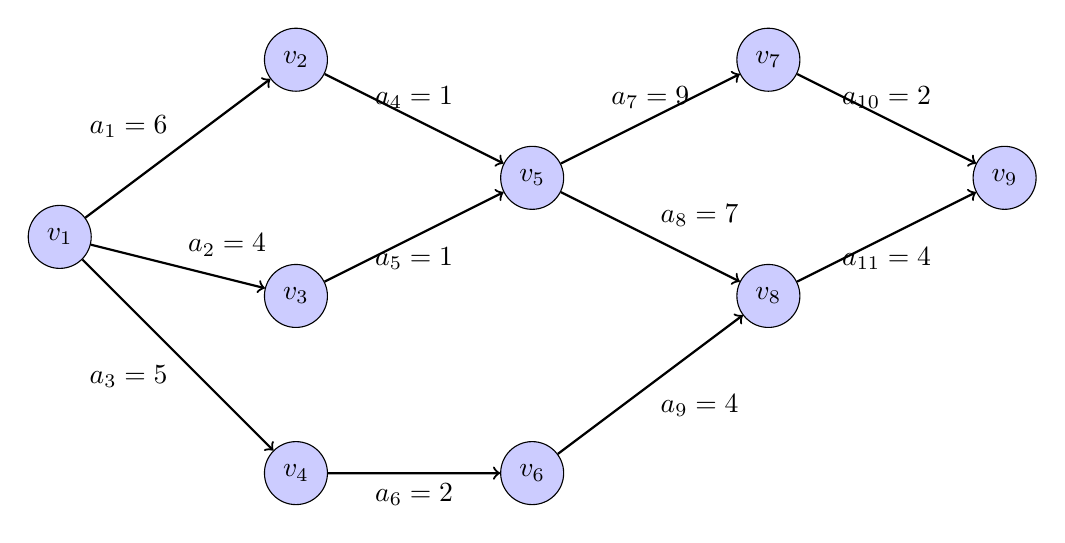
\begin{tikzpicture}[scale=1.5]
    % 定义节点样式
    \tikzstyle{vertex}=[circle,draw,minimum size=0.8cm,fill=blue!20]
    \tikzstyle{edge}=[thick,->]
    
    % 绘制顶点 - 按照用户图片的布局
    \node[vertex] (v1) at (0,0) {$v_1$};
    \node[vertex] (v2) at (2,1.5) {$v_2$};
    \node[vertex] (v3) at (2,-0.5) {$v_3$};
    \node[vertex] (v4) at (2,-2) {$v_4$};
    \node[vertex] (v5) at (4,0.5) {$v_5$};
    \node[vertex] (v6) at (4,-2) {$v_6$};
    \node[vertex] (v7) at (6,1.5) {$v_7$};
    \node[vertex] (v8) at (6,-0.5) {$v_8$};
    \node[vertex] (v9) at (8,0.5) {$v_9$};
    
    % 绘制边(活动)- 按照用户图片的连接方式
    \draw[edge] (v1) -- (v2) node[midway,above left] {$a_1=6$};
    \draw[edge] (v1) -- (v3) node[midway,above right] {$a_2=4$};
    \draw[edge] (v1) -- (v4) node[midway,below left] {$a_3=5$};
    \draw[edge] (v2) -- (v5) node[midway,above] {$a_4=1$};
    \draw[edge] (v3) -- (v5) node[midway,below] {$a_5=1$};
    \draw[edge] (v4) -- (v6) node[midway,below] {$a_6=2$};
    \draw[edge] (v5) -- (v7) node[midway,above] {$a_7=9$};
    \draw[edge] (v5) -- (v8) node[midway,above right] {$a_8=7$};
    \draw[edge] (v6) -- (v8) node[midway,below right] {$a_9=4$};
    \draw[edge] (v7) -- (v9) node[midway,above] {$a_{10}=2$};
    \draw[edge] (v8) -- (v9) node[midway,below] {$a_{11}=4$};
\end{tikzpicture}
\end{center}    

\textbf{关键路径算法步骤}:

\textbf{第一步:计算事件的最早发生时间$ve(i)$}

$ve(i)$表示事件$v_i$的最早发生时间,按拓扑序列从前向后计算:
\begin{align}
ve(1) &= 0 \quad \text{(源点)}\\
ve(2) &= ve(1) + 6 = 0 + 6 = 6\\
ve(3) &= ve(1) + 4 = 0 + 4 = 4\\
ve(4) &= ve(1) + 5 = 0 + 5 = 5\\
ve(5) &= \max\{ve(2) + 1, ve(3) + 1\} = \max\{6+1, 4+1\} = 7\\
ve(6) &= ve(4) + 2 = 5 + 2 = 7\\
ve(7) &= ve(5) + 9 = 7 + 9 = 16\\
ve(8) &= \max\{ve(5) + 7, ve(6) + 4\} = \max\{7+7, 7+4\} = 14\\
ve(9) &= \max\{ve(7) + 2, ve(8) + 4\} = \max\{16+2, 14+4\} = 18
\end{align}

\textbf{第二步:计算事件的最迟发生时间$vl(i)$}

$vl(i)$表示事件$v_i$的最迟发生时间,从汇点开始向前计算:
\begin{align}
vl(9) &= ve(9) = 18 \quad \text{(汇点)}\\
vl(8) &= vl(9) - 4 = 18 - 4 = 14\\
vl(7) &= vl(9) - 2 = 18 - 2 = 16\\
vl(6) &= vl(8) - 4 = 14 - 4 = 10\\
vl(5) &= \min\{vl(7) - 9, vl(8) - 7\} = \min\{16-9, 14-7\} = 7\\
vl(4) &= vl(6) - 2 = 10 - 2 = 8\\
vl(3) &= vl(5) - 1 = 7 - 1 = 6\\
vl(2) &= vl(5) - 1 = 7 - 1 = 6\\
vl(1) &= \min\{vl(2) - 6, vl(3) - 4, vl(4) - 5\} = \min\{6-6, 6-4, 8-5\} = 0
\end{align}

\textbf{第三步:计算活动的最早开始时间$ee(i)$和最迟开始时间$el(i)$}

对于活动$a_k: v_i \rightarrow v_j$,有:
\begin{itemize}
    \item $ee(k) = ve(i)$ (活动的最早开始时间等于起点事件的最早发生时间)
    \item $el(k) = vl(j) - dur(k)$ (活动的最迟开始时间等于终点事件的最迟发生时间减去活动持续时间)
\end{itemize}

\begin{center}
\begin{tabular}{|c|c|c|c|c|c|c|}
\hline
活动 & 起点 & 终点 & 持续时间 & $ee(k)$ & $el(k)$ & $el(k)-ee(k)$ \\
\hline
$a_1$ & $v_1$ & $v_2$ & 6 & $ve(1)=0$ & $vl(2)-6=6-6=0$ & 0 \\
\hline
$a_2$ & $v_1$ & $v_3$ & 4 & $ve(1)=0$ & $vl(3)-4=6-4=2$ & 2 \\
\hline
$a_3$ & $v_1$ & $v_4$ & 5 & $ve(1)=0$ & $vl(4)-5=8-5=3$ & 3 \\
\hline
$a_4$ & $v_2$ & $v_5$ & 1 & $ve(2)=6$ & $vl(5)-1=7-1=6$ & 0 \\
\hline
$a_5$ & $v_3$ & $v_5$ & 1 & $ve(3)=4$ & $vl(5)-1=7-1=6$ & 2 \\
\hline
$a_6$ & $v_4$ & $v_6$ & 2 & $ve(4)=5$ & $vl(6)-2=10-2=8$ & 3 \\
\hline
$a_7$ & $v_5$ & $v_7$ & 9 & $ve(5)=7$ & $vl(7)-9=16-9=7$ & 0 \\
\hline
$a_8$ & $v_5$ & $v_8$ & 7 & $ve(5)=7$ & $vl(8)-7=14-7=7$ & 0 \\
\hline
$a_9$ & $v_6$ & $v_8$ & 4 & $ve(6)=7$ & $vl(8)-4=14-4=10$ & 3 \\
\hline
$a_{10}$ & $v_7$ & $v_9$ & 2 & $ve(7)=16$ & $vl(9)-2=18-2=16$ & 0 \\
\hline
$a_{11}$ & $v_8$ & $v_9$ & 4 & $ve(8)=14$ & $vl(9)-4=18-4=14$ & 0 \\
\hline
\end{tabular}
\end{center}

\textbf{第四步:确定关键路径}

时间余量$d(k) = el(k) - ee(k) = 0$的活动为关键活动:$a_1, a_4, a_7, a_{10}$

\textbf{关键路径}:$v_1 \xrightarrow{a_1} v_2 \xrightarrow{a_4} v_5 \xrightarrow{a_7} v_7 \xrightarrow{a_{10}} v_9$

\textbf{另一条关键路径}:$v_1 \xrightarrow{a_1} v_2 \xrightarrow{a_4} v_5 \xrightarrow{a_8} v_8 \xrightarrow{a_{11}} v_9$

\textbf{工程最短完成时间}:18

\begin{center}
\begin{tikzpicture}[scale=1.5]
    % 定义节点样式
    \tikzstyle{vertex}=[circle,draw,minimum size=0.8cm,fill=blue!20]
    \tikzstyle{critical}=[circle,draw,minimum size=0.8cm,fill=green!30]
    \tikzstyle{critical1}=[circle,draw,minimum size=0.8cm,fill=red!30]
    \tikzstyle{critical2}=[circle,draw,minimum size=0.8cm,fill=blue!30]
    \tikzstyle{edge}=[thick,->]
    \tikzstyle{common_edge}=[very thick,->,green!70!black]
    \tikzstyle{critical_edge1}=[very thick,->,red]
    \tikzstyle{critical_edge2}=[very thick,->,blue]
    
    % 绘制顶点(用不同颜色标记不同关键路径)
    \node[critical] (v1) at (0,0) {$v_1$};        % 共同部分-绿色
    \node[critical] (v2) at (2,1.5) {$v_2$};      % 共同部分-绿色
    \node[vertex] (v3) at (2,-0.5) {$v_3$};       % 非关键顶点
    \node[vertex] (v4) at (2,-2) {$v_4$};         % 非关键顶点
    \node[critical] (v5) at (4,0.5) {$v_5$};      % 共同部分-绿色
    \node[vertex] (v6) at (4,-2) {$v_6$};         % 非关键顶点
    \node[critical1] (v7) at (6,1.5) {$v_7$};     % 关键路径1-红色
    \node[critical2] (v8) at (6,-0.5) {$v_8$};    % 关键路径2-蓝色
    \node[critical] (v9) at (8,0.5) {$v_9$};      % 汇聚点-绿色
    
    % 绘制边(用不同颜色标记不同关键路径)
    \draw[common_edge] (v1) -- (v2) node[midway,above left] {$a_1=6$};      % 共同部分-绿色
    \draw[edge] (v1) -- (v3) node[midway,above right] {$a_2=4$};             % 非关键边
    \draw[edge] (v1) -- (v4) node[midway,below left] {$a_3=5$};              % 非关键边
    \draw[common_edge] (v2) -- (v5) node[midway,above] {$a_4=1$};            % 共同部分-绿色
    \draw[edge] (v3) -- (v5) node[midway,below] {$a_5=1$};                   % 非关键边
    \draw[edge] (v4) -- (v6) node[midway,below] {$a_6=2$};                   % 非关键边
    \draw[critical_edge1] (v5) -- (v7) node[midway,above] {$a_7=9$};         % 关键路径1-红色
    \draw[critical_edge2] (v5) -- (v8) node[midway,above right] {$a_8=7$};   % 关键路径2-蓝色
    \draw[edge] (v6) -- (v8) node[midway,below right] {$a_9=4$};             % 非关键边
    \draw[critical_edge1] (v7) -- (v9) node[midway,above] {$a_{10}=2$};      % 关键路径1-红色
    \draw[critical_edge2] (v8) -- (v9) node[midway,below] {$a_{11}=4$};      % 关键路径2-蓝色
    
    \node at (4,-3) {\textbf{关键路径1:} $v_1 \rightarrow v_2 \rightarrow v_5 \rightarrow v_7 \rightarrow v_9$ \textcolor{red}{(红色)}};
    \node at (4,-3.5) {\textbf{关键路径2:} $v_1 \rightarrow v_2 \rightarrow v_5 \rightarrow v_8 \rightarrow v_9$ \textcolor{blue}{(蓝色)}};
    \node at (4,-4) {\textbf{共同部分:} $v_1 \rightarrow v_2 \rightarrow v_5$ \textcolor{green!70!black}{(绿色)}};
    \node at (4,-4.5) {\textbf{最短完成时间:18}};
\end{tikzpicture}
\end{center}

\textbf{关键路径算法公式总结}:

\begin{enumerate}
    \item \textbf{事件最早发生时间}:
    $$ve(j) = \max_{i \in P(j)} \{ve(i) + dur(i,j)\}$$
    其中$P(j)$表示事件$j$的所有前驱事件集合
    
    \item \textbf{事件最迟发生时间}:
    $$vl(i) = \min_{j \in S(i)} \{vl(j) - dur(i,j)\}$$
    其中$S(i)$表示事件$i$的所有后继事件集合
    
    \item \textbf{活动最早开始时间}:
    $$ee(k) = ve(i) \quad \text{活动}a_k: v_i \rightarrow v_j$$
    
    \item \textbf{活动最迟开始时间}:
    $$el(k) = vl(j) - dur(k) \quad \text{活动}a_k: v_i \rightarrow v_j$$
    
    \item \textbf{活动时间余量}:
    $$d(k) = el(k) - ee(k)$$
    
    \item \textbf{关键活动判定}:
    $$d(k) = 0 \Leftrightarrow \text{活动}a_k\text{是关键活动}$$
\end{enumerate}

\section{习题与解答}

\subsection{基础概念题}

\textbf{题目1}:已知无向图$G$有$n$个顶点$e$条边,求:
\begin{enumerate}
    \item 各顶点度数之和
    \item 若$G$是连通图,$e$的最小值和最大值
    \item 若$G$是完全图,求边数$e$
\end{enumerate}

\textbf{解答1}:
\begin{enumerate}
    \item 根据握手定理:$\sum_{i=0}^{n-1} TD(v_i) = 2e$
    \item 连通图:最小值$e_{min} = n-1$(树),最大值$e_{max} = \frac{n(n-1)}{2}$(完全图)
    \item 完全图:$e = \frac{n(n-1)}{2}$
\end{enumerate}

\textbf{题目2}:设有向图$G=(V,E)$,其中$V=\{v_1,v_2,v_3,v_4\}$,$E=\{\langle v_1,v_2\rangle, \langle v_1,v_3\rangle, \langle v_3,v_4\rangle, \langle v_4,v_1\rangle\}$,画出该图的邻接矩阵和邻接表。

\textbf{解答2}:

邻接矩阵:
$$
\begin{bmatrix}
0 & 1 & 1 & 0 \\
0 & 0 & 0 & 0 \\
0 & 0 & 0 & 1 \\
1 & 0 & 0 & 0
\end{bmatrix}
$$

邻接表:
\begin{align}
v_1 &: \rightarrow v_2 \rightarrow v_3 \rightarrow NULL \\
v_2 &: \rightarrow NULL \\
v_3 &: \rightarrow v_4 \rightarrow NULL \\
v_4 &: \rightarrow v_1 \rightarrow NULL
\end{align}

\subsection{算法应用题}

\textbf{题目3}:对下图从顶点$A$开始进行DFS和BFS遍历,写出遍历序列。

\begin{center}
\begin{tikzpicture}[scale=1.2]
    \node[circle,draw,minimum size=0.8cm] (A) at (0,2) {A};
    \node[circle,draw,minimum size=0.8cm] (B) at (2,2) {B};
    \node[circle,draw,minimum size=0.8cm] (C) at (4,2) {C};
    \node[circle,draw,minimum size=0.8cm] (D) at (0,0) {D};
    \node[circle,draw,minimum size=0.8cm] (E) at (2,0) {E};
    \node[circle,draw,minimum size=0.8cm] (F) at (4,0) {F};
    
    \draw (A) -- (B);
    \draw (A) -- (D);
    \draw (B) -- (C);
    \draw (B) -- (E);
    \draw (C) -- (F);
    \draw (D) -- (E);
    \draw (E) -- (F);
\end{tikzpicture}
\end{center}

\textbf{解答3}:

DFS遍历序列(按字母顺序选择邻接点):$A \rightarrow B \rightarrow C \rightarrow F \rightarrow E \rightarrow D$

BFS遍历序列:$A \rightarrow B \rightarrow D \rightarrow C \rightarrow E \rightarrow F$

\textbf{题目4}:用Prim算法求下图的最小生成树,写出构造过程。

\begin{center}
\begin{tikzpicture}[scale=1.5]
    \node[circle,draw,minimum size=0.8cm] (A) at (0,1.5) {A};
    \node[circle,draw,minimum size=0.8cm] (B) at (1.5,3) {B};
    \node[circle,draw,minimum size=0.8cm] (C) at (3,1.5) {C};
    \node[circle,draw,minimum size=0.8cm] (D) at (1.5,0) {D};
    
    \draw (A) -- node[above left] {5} (B);
    \draw (A) -- node[below] {3} (D);
    \draw (B) -- node[above] {6} (C);
    \draw (C) -- node[right] {2} (D);
    \draw (A) -- node[above] {4} (C);
    \draw (B) -- node[left] {7} (D);
\end{tikzpicture}
\end{center}

\textbf{解答4}:

从顶点$A$开始:

\begin{table}[h]
\centering
\begin{tabular}{|c|c|c|c|c|c|}
\hline
\textbf{步骤} & \textbf{U} & \textbf{选择的边} & \textbf{权值} & \textbf{lowcost更新} & \textbf{总权值} \\
\hline
初始 & $\{A\}$ & - & - & B:5, C:4, D:3 & 0 \\
\hline
1 & $\{A,D\}$ & $(A,D)$ & 3 & B:5, C:2 & 3 \\
\hline
2 & $\{A,D,C\}$ & $(D,C)$ & 2 & B:5 & 5 \\
\hline
3 & $\{A,D,C,B\}$ & $(A,B)$ & 5 & - & 10 \\
\hline
\end{tabular}
\end{table}

最小生成树包含边:$(A,D)$,$(D,C)$,$(A,B)$,总权值为10。

\textbf{题目5}:用Dijkstra算法求从顶点$S$到其他各顶点的最短路径。

\begin{center}
\begin{tikzpicture}[scale=1.2]
    \node[circle,draw,minimum size=0.8cm] (S) at (0,1) {S};
    \node[circle,draw,minimum size=0.8cm] (A) at (2,2) {A};
    \node[circle,draw,minimum size=0.8cm] (B) at (2,0) {B};
    \node[circle,draw,minimum size=0.8cm] (C) at (4,2) {C};
    \node[circle,draw,minimum size=0.8cm] (D) at (4,0) {D};
    \node[circle,draw,minimum size=0.8cm] (T) at (6,1) {T};
    
    \draw[-latex] (S) -- node[above left] {2} (A);
    \draw[-latex] (S) -- node[below left] {5} (B);
    \draw[-latex] (A) -- node[above] {3} (C);
    \draw[-latex] (A) -- node[left] {4} (B);
    \draw[-latex] (B) -- node[below] {1} (D);
    \draw[-latex] (C) -- node[above right] {2} (T);
    \draw[-latex] (D) -- node[below right] {6} (T);
    \draw[-latex] (B) -- node[above right] {7} (C);
\end{tikzpicture}
\end{center}

\textbf{解答5}:

Dijkstra算法执行过程:

\begin{table}[h]
\centering
\begin{tabular}{|c|c|c|c|c|c|c|c|}
\hline
\textbf{步骤} & \textbf{S集合} & \textbf{选择顶点} & \textbf{A} & \textbf{B} & \textbf{C} & \textbf{D} & \textbf{T} \\
\hline
初始 & $\{S\}$ & - & 2 & 5 & $\infty$ & $\infty$ & $\infty$ \\
\hline
1 & $\{S,A\}$ & A & - & 5 & 5 & $\infty$ & $\infty$ \\
\hline
2 & $\{S,A,B\}$ & B & - & - & 5 & 6 & $\infty$ \\
\hline
3 & $\{S,A,B,C\}$ & C & - & - & - & 6 & 7 \\
\hline
4 & $\{S,A,B,C,D\}$ & D & - & - & - & - & 7 \\
\hline
5 & $\{S,A,B,C,D,T\}$ & T & - & - & - & - & - \\
\hline
\end{tabular}
\end{table}

最短路径:
\begin{itemize}
    \item $S \rightarrow A$:距离2,路径:$S \rightarrow A$
    \item $S \rightarrow B$:距离5,路径:$S \rightarrow B$
    \item $S \rightarrow C$:距离5,路径:$S \rightarrow A \rightarrow C$
    \item $S \rightarrow D$:距离6,路径:$S \rightarrow B \rightarrow D$
    \item $S \rightarrow T$:距离7,路径:$S \rightarrow A \rightarrow C \rightarrow T$
\end{itemize}

\subsection{综合分析题}

\textbf{题目6}:某项目包含活动$A, B, C, D, E, F$,活动间的依赖关系如下:
\begin{itemize}
    \item 活动$A$:无前驱,持续时间3天
    \item 活动$B$:依赖$A$,持续时间4天
    \item 活动$C$:依赖$A$,持续时间2天
    \item 活动$D$:依赖$B, C$,持续时间5天
    \item 活动$E$:依赖$C$,持续时间3天
    \item 活动$F$:依赖$D, E$,持续时间2天
\end{itemize}

画出AOE网图,求关键路径和最短工期。

\textbf{解答6}:

AOE网图:

\begin{center}
\begin{tikzpicture}[scale=1.2]
    \node[circle,draw,minimum size=0.8cm] (v0) at (0,1) {$v_0$};
    \node[circle,draw,minimum size=0.8cm] (v1) at (2,1) {$v_1$};
    \node[circle,draw,minimum size=0.8cm] (v2) at (4,2) {$v_2$};
    \node[circle,draw,minimum size=0.8cm] (v3) at (4,0) {$v_3$};
    \node[circle,draw,minimum size=0.8cm] (v4) at (6,1.5) {$v_4$};
    \node[circle,draw,minimum size=0.8cm] (v5) at (6,0.5) {$v_5$};
    \node[circle,draw,minimum size=0.8cm] (v6) at (8,1) {$v_6$};
    
    \draw[-latex] (v0) -- node[above] {A/3} (v1);
    \draw[-latex] (v1) -- node[above] {B/4} (v2);
    \draw[-latex] (v1) -- node[below] {C/2} (v3);
    \draw[-latex] (v2) -- node[above] {D/5} (v4);
    \draw[-latex] (v3) -- node[right] {D/5} (v4);
    \draw[-latex] (v3) -- node[below] {E/3} (v5);
    \draw[-latex] (v4) -- node[above] {F/2} (v6);
    \draw[-latex] (v5) -- node[below] {F/2} (v6);
\end{tikzpicture}
\end{center}

计算过程:

事件最早发生时间$ve$:
\begin{align}
ve[v_0] &= 0 \\
ve[v_1] &= 3 \\
ve[v_2] &= 7 \\
ve[v_3] &= 5 \\
ve[v_4] &= \max(12, 10) = 12 \\
ve[v_5] &= 8 \\
ve[v_6] &= \max(14, 10) = 14
\end{align}

事件最迟发生时间$vl$:
\begin{align}
vl[v_6] &= 14 \\
vl[v_5] &= 12 \\
vl[v_4] &= 12 \\
vl[v_3] &= \min(7, 9) = 7 \\
vl[v_2] &= 7 \\
vl[v_1] &= \min(3, 5) = 3 \\
vl[v_0] &= 0
\end{align}

关键活动判断($ee = el$):
\begin{itemize}
    \item 活动$A$:$ee = 0, el = 0$ ✓
    \item 活动$B$:$ee = 3, el = 3$ ✓
    \item 活动$C$:$ee = 3, el = 5$ ✗
    \item 活动$D$:$ee = 7, el = 7$ ✓
    \item 活动$E$:$ee = 5, el = 9$ ✗
    \item 活动$F$:$ee = 12, el = 12$ ✓
\end{itemize}

\textbf{结果}:
\begin{itemize}
    \item 关键路径:$v_0 \rightarrow v_1 \rightarrow v_2 \rightarrow v_4 \rightarrow v_6$
    \item 关键活动:$A \rightarrow B \rightarrow D \rightarrow F$
    \item 最短工期:14天
\end{itemize}

\subsection{计算题强化训练}

\textbf{题目7}:设无向图$G$有6个顶点,各顶点的度数分别为:2, 3, 3, 3, 4, 5。
\begin{enumerate}
    \item 验证是否满足握手定理
    \item 画出一个满足条件的图
    \item 该图最少有几个连通分量?
\end{enumerate}

\textbf{解答7}:
\begin{enumerate}
    \item 度数和:$2 + 3 + 3 + 3 + 4 + 5 = 20 = 2 \times 10$,满足握手定理,边数$e = 10$
    \item 可以构造满足条件的图(画图略)
    \item 最少1个连通分量(因为度数和为偶数且每个顶点度数都不为0)
\end{enumerate}

\textbf{题目8}:比较邻接矩阵和邻接表在以下操作的时间复杂度:
\begin{enumerate}
    \item 判断顶点$i$和$j$是否邻接
    \item 求顶点$i$的所有邻接点
    \item 在图中插入一个新顶点
    \item 删除顶点$i$
\end{enumerate}

\textbf{解答8}:

\begin{table}[h]
\centering
\begin{tabular}{|l|c|c|}
\hline
\textbf{操作} & \textbf{邻接矩阵} & \textbf{邻接表} \\
\hline
判断$(i,j)$是否邻接 & $O(1)$ & $O(度数)$ \\
\hline
求顶点$i$的所有邻接点 & $O(n)$ & $O(度数)$ \\
\hline
插入新顶点 & $O(n^2)$ & $O(1)$ \\
\hline
删除顶点$i$ & $O(n^2)$ & $O(n+e)$ \\
\hline
\end{tabular}
\end{table}

这些习题涵盖了图论的核心概念和算法,通过练习可以加深对知识点的理解和应用能力。建议结合教材和课堂讲解,多做手工模拟以掌握算法的执行过程。

\end{document} 
\part{查找技术}
\documentclass[12pt,a4paper]{amsart}
\usepackage[utf8]{inputenc}
\usepackage[T1]{fontenc}
\usepackage{amsmath,amsfonts,amssymb}
\usepackage{tikz}
\usepackage{algorithm}
\usepackage{algorithmic}
\usepackage{listings}
\usepackage{xcolor}
\usepackage{geometry}
\usepackage{fancyhdr}
\usepackage{enumitem}
\usepackage{booktabs}
\usepackage{multirow}
\usepackage[hidelinks,bookmarksnumbered,bookmarksopen]{hyperref}
\usepackage{xeCJK}
\setCJKmainfont{LXGW WenKai}

% 页面设置
\geometry{left=2cm,right=2cm,top=2.5cm,bottom=2.5cm}
\pagestyle{fancy}
\fancyhf{}
\fancyhead[L]{查找技术复习总结}
\fancyhead[R]{\thepage}

% TikZ库
\usetikzlibrary{arrows,positioning,shapes,calc,trees,graphs}

% 代码高亮设置
\lstset{
    language=C++,
    basicstyle=\ttfamily\small,
    keywordstyle=\color{blue}\bfseries,
    commentstyle=\color{green!60!black},
    stringstyle=\color{red},
    numbers=left,
    numberstyle=\tiny\color{gray},
    stepnumber=1,
    numbersep=10pt,
    backgroundcolor=\color{gray!10},
    frame=single,
    tabsize=4,
    captionpos=b,
    breaklines=true,
    breakatwhitespace=false,
    showspaces=false,
    showstringspaces=false,
    showtabs=false
}

% 定理环境
\newtheorem{definition}{定义}[section]
\newtheorem{theorem}{定理}[section]
\newtheorem{algorithm_desc}{算法}[section]
\newtheorem{example}{例题}[section]

\title{\textbf{数据结构第七章:查找技术复习总结}}
\author{期末考试复习资料}
\date{\today}

\begin{document}

% \maketitle

% % 目录设置
% \tableofcontents
% \newpage

\section{查找的基本概念}

\subsection{基本术语与定义}

\begin{definition}[记录与关键码]
在查找问题中,通常将数据元素称为\textbf{记录}(record)。可以标识一个记录的某个数据项称为\textbf{关键码}(key),关键码的值称为\textbf{键值}(keyword)。若关键码可以唯一标识一个记录,则称此关键码为\textbf{主关键码}(primary key);反之,称此关键码为\textbf{次关键码}(second key)。
\end{definition}

\begin{center}
\begin{tikzpicture}[scale=1.2]
    % 记录结构示意图
    \node[draw,rectangle,minimum width=6cm,minimum height=0.8cm] (record) at (0,0) {记录};
    \node[draw,rectangle,minimum width=1.2cm,minimum height=0.6cm,fill=red!20] (key) at (-2,-1.2) {关键码};
    \node[draw,rectangle,minimum width=1.2cm,minimum height=0.6cm,fill=blue!20] (data1) at (-0.5,-1.2) {数据1};
    \node[draw,rectangle,minimum width=1.2cm,minimum height=0.6cm,fill=blue!20] (data2) at (1,-1.2) {数据2};
    \node[draw,rectangle,minimum width=1.2cm,minimum height=0.6cm,fill=blue!20] (data3) at (2.5,-1.2) {数据3};
    
    \draw[->] (record.south) -- (key.north);
    \draw[->] (record.south) -- (data1.north);
    \draw[->] (record.south) -- (data2.north);
    \draw[->] (record.south) -- (data3.north);
    
    \node at (0,-2.2) {\textbf{记录结构示意图}};
\end{tikzpicture}
\end{center}

\begin{definition}[查找]
广义地讲,查找(search)是在具有相同类型的记录构成的集合中找出满足给定条件的记录。若在查找集合中找到了与给定值相等的记录,则称\textbf{查找成功};否则称\textbf{查找不成功}(或查找失败)。
\end{definition}

\begin{definition}[静态查找与动态查找]
不涉及插入和删除操作的查找称为\textbf{静态查找}(static search),静态查找在查找不成功时,只返回一个不成功标志,查找的结果不改变查找集合;涉及插入和删除操作的查找称为\textbf{动态查找}(dynamic search),动态查找在查找不成功时,需要将被查找的记录插入到查找集合中。
\end{definition}

\subsection{查找算法的性能分析}

\begin{definition}[平均查找长度]
查找算法的基本操作通常是将记录和给定值进行比较,所以,通常以记录的平均比较次数来度量查找算法的平均时间性能,称为\textbf{平均查找长度}(Average Search Length, ASL)。对于查找成功的情况,其计算公式为:
\begin{equation}
\text{ASL} = \sum_{i=1}^{n} p_i c_i
\end{equation}
其中,$n$为问题规模,查找集合中的记录个数;$p_i$为查找第$i$个记录的概率;$c_i$为查找第$i$个记录所需的比较次数。
\end{definition}

\section{线性表的查找技术}

\subsection{顺序查找}

\begin{definition}[顺序查找]
顺序查找(sequential search)又称线性查找,其基本思想为:从线性表的一端向另一端逐个将记录与给定值进行比较,若相等,则查找成功,给出该记录在表中的位置;若整个表检测完仍未找到与给定值相等的记录,则查找失败。
\end{definition}

\begin{algorithm}
\caption{顺序查找(带哨兵)}
\begin{algorithmic}[1]
\REQUIRE 查找表$data[1..n]$,待查值$k$
\ENSURE 查找成功返回位置,失败返回0
\STATE $i \leftarrow n$ \COMMENT{从表高端开始}
\STATE $data[0] \leftarrow k$ \COMMENT{设置哨兵}
\WHILE{$data[i] \neq k$}
    \STATE $i \leftarrow i - 1$
\ENDWHILE
\RETURN $i$
\end{algorithmic}
\end{algorithm}

\begin{theorem}[顺序查找的性能]
设每个记录的查找概率相等,即$p_i = 1/n \quad (1 \leq i \leq n)$,则:
\begin{itemize}
\item 查找成功时的平均查找长度:
\begin{equation}
\text{ASL}_{\text{成功}} = \frac{1}{n}\sum_{i=1}^{n}(n-i+1) = \frac{n+1}{2} = O(n)
\end{equation}
\item 查找失败时的平均查找长度:
\begin{equation}
\text{ASL}_{\text{失败}} = n+1 = O(n)
\end{equation}
\end{itemize}
\end{theorem}

\subsection{折半查找}

\begin{definition}[折半查找]
折半查找(binary search)的基本思想是:假设有序表按关键码升序排列,取中间记录作为比较对象,若给定值与中间记录相等,则查找成功;若给定值小于中间记录,则在有序表的左半区继续查找;若给定值大于中间记录,则在有序表的右半区继续查找。
\end{definition}

\begin{algorithm}
\caption{折半查找(非递归)}
\begin{algorithmic}[1]
\REQUIRE 有序表$data[1..n]$,待查值$k$
\ENSURE 查找成功返回位置,失败返回0
\STATE $low \leftarrow 1, high \leftarrow n$
\WHILE{$low \leq high$}
    \STATE $mid \leftarrow \lfloor(low + high)/2\rfloor$
    \IF{$k < data[mid]$}
        \STATE $high \leftarrow mid - 1$
    \ELSIF{$k > data[mid]$}
        \STATE $low \leftarrow mid + 1$
    \ELSE
        \RETURN $mid$
    \ENDIF
\ENDWHILE
\RETURN $0$
\end{algorithmic}
\end{algorithm}

\begin{theorem}[折半查找的性能]
设判定树是深度为$k$的满二叉树$(n = 2^k - 1)$,若有序表中每个记录的查找概率相等,即$p_i = 1/n \quad (1 \leq i \leq n)$,则折半查找的平均查找长度为:
\begin{equation}
\text{ASL} = \frac{1}{n}\sum_{j=1}^{k} j \times 2^{j-1} \approx \log_2(n+1) - 1 = O(\log n)
\end{equation}
\end{theorem}

\begin{example}[折半查找过程]
在有序表$\{7,14,18,21,23,29,31,35,38\}$中查找18:
\begin{enumerate}
\item 初始:$low=1, high=9, mid=5$,$data[5]=23 > 18$,令$high=4$
\item $low=1, high=4, mid=2$,$data[2]=14 < 18$,令$low=3$
\item $low=3, high=4, mid=3$,$data[3]=18 = 18$,查找成功
\end{enumerate}
比较次数:3次
\end{example}

\section{树表的查找技术}

\subsection{二叉排序树}

\begin{definition}[二叉排序树]
二叉排序树(Binary Sort Tree, BST)又称二叉查找树,或者是一棵空的二叉树,或者是具有下列性质的二叉树:
\begin{enumerate}
\item 若左子树不空,则左子树上所有结点的值均小于根结点的值;
\item 若右子树不空,则右子树上所有结点的值均大于根结点的值;
\item 左右子树也都是二叉排序树。
\end{enumerate}
\end{definition}

\begin{center}
\begin{tikzpicture}[level distance=1.5cm,
level 1/.style={sibling distance=4cm},
level 2/.style={sibling distance=2cm},
level 3/.style={sibling distance=1.5cm}]
\node [circle,draw] {50}
    child {node [circle,draw] {30}
        child {node [circle,draw] {20}
            child {node [circle,draw] {10}}
            child[missing]}
        child {node [circle,draw] {40}
            child[missing] 
            child {node [circle,draw] {45}}}}
    child {node [circle,draw] {70}
        child {node [circle,draw] {60}}
        child {node [circle,draw] {80}
            child[missing]
            child {node [circle,draw] {90}}}};
\node at (0,-5) {\textbf{二叉排序树示例}};
\end{tikzpicture}
\end{center}

\begin{algorithm}
\caption{二叉排序树查找}
\begin{algorithmic}[1]
\REQUIRE 二叉排序树根结点$T$,待查关键码$k$
\ENSURE 查找成功返回结点指针,失败返回NULL
\IF{$T = NULL$ or $k = T \rightarrow key$}
    \RETURN $T$
\ELSIF{$k < T \rightarrow key$}
    \RETURN BSTSearch($T \rightarrow lchild, k$)
\ELSE
    \RETURN BSTSearch($T \rightarrow rchild, k$)
\ENDIF
\end{algorithmic}
\end{algorithm}

\begin{algorithm}
\caption{二叉排序树插入}
\begin{algorithmic}[1]
\REQUIRE 二叉排序树根结点$T$,待插入关键码$k$
\ENSURE 插入成功返回TRUE,失败返回FALSE
\IF{$T = NULL$}
    \STATE 创建新结点,关键码为$k$
    \RETURN TRUE
\ELSIF{$k = T \rightarrow key$}
    \RETURN FALSE \COMMENT{关键码已存在}
\ELSIF{$k < T \rightarrow key$}
    \RETURN BSTInsert($T \rightarrow lchild, k$)
\ELSE
    \RETURN BSTInsert($T \rightarrow rchild, k$)
\ENDIF
\end{algorithmic}
\end{algorithm}

\begin{theorem}[二叉排序树性能]
二叉排序树查找的时间复杂度:
\begin{itemize}
\item 最好情况(完全二叉树):$O(\log n)$
\item 最坏情况(单支树):$O(n)$
\item 平均情况:$O(\log n)$
\end{itemize}
\end{theorem}

\subsection{平衡二叉树(AVL树)}

\begin{definition}[平衡二叉树]
平衡二叉树(Balanced Binary Tree)或AVL树是一种特殊的二叉排序树,满足:
\begin{enumerate}
\item 是一棵二叉排序树;
\item 对任意结点,其左右子树的高度差的绝对值不超过1。
\end{enumerate}
结点的\textbf{平衡因子}(Balance Factor, BF)定义为该结点左子树的高度减去右子树的高度。AVL树中任一结点的平衡因子只能是-1、0或1。
\end{definition}

\begin{center}
\begin{tikzpicture}[level distance=1.2cm,
level 1/.style={sibling distance=2cm},
level 2/.style={sibling distance=1cm}]
% 失衡情况:LL型
\node at (-6,2) {\textbf{LL型失衡}};
\node[circle,draw,minimum size=8mm] at (-6,0) {$C$}
    child {node[circle,draw,minimum size=8mm] {$B$}
        child {node[circle,draw,minimum size=8mm] {$A$}}
        child[missing]}
    child[missing];
\node at (-6,-2.8) {失衡};

% 调整后
\node at (-2.5,2) {\textbf{右旋调整}};
\node[circle,draw,minimum size=8mm] at (-2.5,0) {$B$}
    child {node[circle,draw,minimum size=8mm] {$A$}}
    child {node[circle,draw,minimum size=8mm] {$C$}};
\node at (-2.5,-2.8) {平衡};

\draw[->,thick] (-4.8,0) -- (-3.2,0);

% 失衡情况:RR型
\node at (1.5,2) {\textbf{RR型失衡}};
\node[circle,draw,minimum size=8mm] at (1.5,0) {$A$}
    child[missing]
    child {node[circle,draw,minimum size=8mm] {$B$}
        child[missing]
        child {node[circle,draw,minimum size=8mm] {$C$}}};
\node at (1.5,-2.8) {失衡};

% 调整后
\node at (5,2) {\textbf{左旋调整}};
\node[circle,draw,minimum size=8mm] at (5,0) {$B$}
    child {node[circle,draw,minimum size=8mm] {$A$}}
    child {node[circle,draw,minimum size=8mm] {$C$}};
\node at (5,-2.8) {平衡};

\draw[->,thick] (3.2,0) -- (3.8,0);
\end{tikzpicture}
\end{center}

\begin{center}
\begin{tikzpicture}[level distance=1.2cm,
level 1/.style={sibling distance=2cm},
level 2/.style={sibling distance=1cm}]
% 失衡情况:LR型
\node at (-3.5,2) {\textbf{LR型失衡}};
\node[circle,draw,minimum size=8mm] at (-3.5,0) {$C$}
    child {node[circle,draw,minimum size=8mm] {$A$}
        child[missing]
        child {node[circle,draw,minimum size=8mm] {$B$}}}
    child[missing];
\node at (-3.5,-2.8) {失衡};

% 调整后
\node at (-0.5,2) {\textbf{左旋-右旋调整}};
\node[circle,draw,minimum size=8mm] at (-0.5,0) {$B$}
    child {node[circle,draw,minimum size=8mm] {$A$}}
    child {node[circle,draw,minimum size=8mm] {$C$}};
\node at (-0.5,-2.8) {平衡};

\draw[->,thick] (-2.3,0) -- (-1.7,0);

% 失衡情况:RL型
\node at (2.5,2) {\textbf{RL型失衡}};
\node[circle,draw,minimum size=8mm] at (2.5,0) {$A$}
    child[missing]
    child {node[circle,draw,minimum size=8mm] {$C$}
        child {node[circle,draw,minimum size=8mm] {$B$}}
        child[missing]};
\node at (2.5,-2.8) {失衡};

% 调整后
\node at (5.5,2) {\textbf{右旋-左旋调整}};
\node[circle,draw,minimum size=8mm] at (5.5,0) {$B$}
    child {node[circle,draw,minimum size=8mm] {$A$}}
    child {node[circle,draw,minimum size=8mm] {$C$}};
\node at (5.5,-2.8) {平衡};

\draw[->,thick] (3.7,0) -- (4.3,0);
\end{tikzpicture}
\end{center}

\begin{example}[平衡二叉树构建示例]
按顺序$\{10,24,32,80,55,30\}$构建平衡二叉树的过程:

给定插入顺序:$\{10, 24, 32, 80, 55, 30\}$

\textbf{步骤1:插入10}
\begin{center}
\begin{tikzpicture}[level distance=1.2cm]
\node[circle,draw,minimum size=8mm] {$10$};
\end{tikzpicture}
\end{center}
\begin{center}
根节点:10,平衡因子:0,树平衡
\end{center}

\textbf{步骤2:插入24}
\begin{center}
\begin{tikzpicture}[level distance=1.2cm]
\node[circle,draw,minimum size=8mm] {$10$}
    child[missing]
    child {node[circle,draw,minimum size=8mm] {$24$}};
\end{tikzpicture}
\end{center}
\begin{center}
根节点:10,平衡因子:$BF(10) = 0 - 1 = -1$,$BF(24) = 0$,树平衡
\end{center}

\textbf{步骤3:插入32}
\begin{center}
\begin{tikzpicture}[level distance=1.2cm]
\node[circle,draw,minimum size=8mm] {$10$}
    child[missing]
    child {node[circle,draw,minimum size=8mm] {$24$}
        child[missing]
        child {node[circle,draw,minimum size=8mm] {$32$}}};
\end{tikzpicture}
\end{center}
\begin{center}
根节点:10,平衡因子:$BF(10) = 0 - 2 = -2$,$BF(24) = -1$,$BF(32) = 0$
\end{center}
\begin{center}
\textcolor{red}{节点10失衡!RR型不平衡,需要左旋}
\end{center}

\textbf{左旋调整后(以24为轴):}
\begin{center}
\begin{tikzpicture}[level distance=1.2cm,
level 1/.style={sibling distance=2cm}]
\node[circle,draw,minimum size=8mm] {$24$}
    child {node[circle,draw,minimum size=8mm] {$10$}}
    child {node[circle,draw,minimum size=8mm] {$32$}};
\end{tikzpicture}
\end{center}
\begin{center}
根节点:24,所有节点平衡因子为0,树平衡
\end{center}

\textbf{步骤4:插入80}
\begin{center}
\begin{tikzpicture}[level distance=1.2cm,
level 1/.style={sibling distance=2cm}]
\node[circle,draw,minimum size=8mm] {$24$}
    child {node[circle,draw,minimum size=8mm] {$10$}}
    child {node[circle,draw,minimum size=8mm] {$32$}
        child[missing]
        child {node[circle,draw,minimum size=8mm] {$80$}}};
\end{tikzpicture}
\end{center}
\begin{center}
根节点:24,平衡因子:$BF(24) = 1 - 2 = -1$,$BF(32) = -1$,树平衡
\end{center}

\textbf{步骤5:插入55}
\begin{center}
\begin{tikzpicture}[level distance=1.2cm,
level 1/.style={sibling distance=2cm},
level 2/.style={sibling distance=1cm}]
\node[circle,draw,minimum size=8mm] {$24$}
    child {node[circle,draw,minimum size=8mm] {$10$}}
    child {node[circle,draw,minimum size=8mm] {$32$}
        child[missing]
        child {node[circle,draw,minimum size=8mm] {$80$}
            child {node[circle,draw,minimum size=8mm] {$55$}}
            child[missing]}};
\end{tikzpicture}
\end{center}
\begin{center}
根节点:24,平衡因子:$BF(32) = 0 - 2 = -2$,$BF(80) = 1$
\end{center}
\begin{center}
\textcolor{red}{节点32失衡!RL型不平衡,需要RL旋转}
\end{center}

\textbf{RL型调整:对80先右旋,再对32左旋}
\begin{center}
\begin{tikzpicture}[level distance=1.2cm,
level 1/.style={sibling distance=2.5cm},
level 2/.style={sibling distance=1.2cm}]
\node[circle,draw,minimum size=8mm] {$24$}
    child {node[circle,draw,minimum size=8mm] {$10$}}
    child {node[circle,draw,minimum size=8mm] {$55$}
        child {node[circle,draw,minimum size=8mm] {$32$}}
        child {node[circle,draw,minimum size=8mm] {$80$}}};
\end{tikzpicture}
\end{center}
\begin{center}
根节点:24,所有节点平衡,树平衡
\end{center}

\textbf{步骤6:插入30}
\begin{center}
\begin{tikzpicture}[level distance=1.2cm,
level 1/.style={sibling distance=2.5cm},
level 2/.style={sibling distance=1.2cm}]
\node[circle,draw,minimum size=8mm] {$24$}
    child {node[circle,draw,minimum size=8mm] {$10$}}
    child {node[circle,draw,minimum size=8mm] {$55$}
        child {node[circle,draw,minimum size=8mm] {$32$}
            child {node[circle,draw,minimum size=8mm] {$30$}}
            child[missing]}
        child {node[circle,draw,minimum size=8mm] {$80$}}};
\end{tikzpicture}
\end{center}
\begin{center}
根节点:24,平衡因子:$BF(24) = 1 - 3 = -2$,$BF(55) = 2 - 1 = 1$,$BF(32) = 1$
\end{center}
\begin{center}
\textcolor{red}{节点24失衡!需要左旋调整}
\end{center}

\textbf{左旋调整过程:以55为新根}
\begin{center}
\begin{tikzpicture}[level distance=1.2cm,
level 1/.style={sibling distance=3cm},
level 2/.style={sibling distance=1.5cm}]
\node[circle,draw,minimum size=8mm] {$55$}
    child {node[circle,draw,minimum size=8mm] {$24$}
        child {node[circle,draw,minimum size=8mm] {$10$}}
        child {node[circle,draw,minimum size=8mm] {$32$}
            child {node[circle,draw,minimum size=8mm] {$30$}}
            child[missing]}}
    child {node[circle,draw,minimum size=8mm] {$80$}};
\end{tikzpicture}
\end{center}
\begin{center}
根节点:55,所有节点平衡因子在[-1,1]范围内,树平衡
\end{center}

等等,让我重新分析步骤6的旋转。实际上应该进行如下操作:

\textbf{重新分析步骤6:插入30后的调整}
插入30后,节点24的平衡因子变为-2,这是一个复杂的情况。路径是24→55→32→30,这构成RL型不平衡。

\textbf{正确的RL型调整:}
\begin{enumerate}
\item 先对55的左子树32进行右旋
\item 再对24进行左旋,以调整后的节点为轴
\end{enumerate}

经过正确的RL旋转后:
\begin{center}
\begin{tikzpicture}[level distance=1.2cm,
level 1/.style={sibling distance=2.5cm},
level 2/.style={sibling distance=1.2cm}]
\node[circle,draw,minimum size=8mm] {$32$}
    child {node[circle,draw,minimum size=8mm] {$24$}
        child {node[circle,draw,minimum size=8mm] {$10$}}
        child {node[circle,draw,minimum size=8mm] {$30$}}}
    child {node[circle,draw,minimum size=8mm] {$55$}
        child[missing]
        child {node[circle,draw,minimum size=8mm] {$80$}}};
\end{tikzpicture}
\end{center}

\textbf{最终的平衡二叉树:}
\begin{center}
\begin{tikzpicture}[level distance=1.2cm,
level 1/.style={sibling distance=2.5cm},
level 2/.style={sibling distance=1.2cm}]
\node[circle,draw,minimum size=8mm] {$32$}
    child {node[circle,draw,minimum size=8mm] {$24$}
        child {node[circle,draw,minimum size=8mm] {$10$}}
        child {node[circle,draw,minimum size=8mm] {$30$}}}
    child {node[circle,draw,minimum size=8mm] {$55$}
        child[missing]
        child {node[circle,draw,minimum size=8mm] {$80$}}};
\end{tikzpicture}
\end{center}
\begin{center}
\textcolor{green}{最终根节点为32,所有节点都平衡!}
\end{center}

\textbf{答案:B. 32}

\textbf{解释:}在平衡二叉树的构建过程中,通过一系列的旋转操作来维持树的平衡性。最终构建完成的平衡二叉树的根节点是32。
\end{example}


\subsection{B树}

\begin{definition}[m阶B树]
一棵m阶B树(B-tree)或为空树,或为满足下列性质的m叉树:
\begin{enumerate}
\item 树中每个结点最多含有$m$个孩子($m \geq 2$);
\item 若根结点不是叶子结点,则至少有2个孩子;
\item 除根结点和叶子结点外,其它每个结点至少有$\lceil m/2 \rceil$个孩子;
\item 所有叶子结点出现在同一层,叶子结点不包含任何信息;
\item 有$k$个孩子的非叶子结点有$k-1$个关键码,关键码按升序排列。
\end{enumerate}
\end{definition}

\begin{center}
\begin{tikzpicture}[level distance=2cm,
level 1/.style={sibling distance=6cm},
level 2/.style={sibling distance=2cm}]
% 3阶B树示例
\node[rectangle,draw,minimum width=2cm] {$20 \mid 50$}
    child {node[rectangle,draw,minimum width=1.5cm] {$10$}
        child {node[rectangle,draw,minimum width=0.8cm] {$5$}}
        child {node[rectangle,draw,minimum width=0.8cm] {$15$}}}
    child {node[rectangle,draw,minimum width=1.5cm] {$30 \mid 40$}
        child {node[rectangle,draw,minimum width=0.8cm] {$25$}}
        child {node[rectangle,draw,minimum width=0.8cm] {$35$}}
        child {node[rectangle,draw,minimum width=0.8cm] {$45$}}}
    child {node[rectangle,draw,minimum width=1.5cm] {$60 \mid 70$}
        child {node[rectangle,draw,minimum width=0.8cm] {$55$}}
        child {node[rectangle,draw,minimum width=0.8cm] {$65$}}
        child {node[rectangle,draw,minimum width=0.8cm] {$75$}}};
\node at (0,-4.5) {\textbf{3阶B树示例}};
\end{tikzpicture}
\end{center}

\section{散列表查找技术}

\subsection{散列表的基本概念}

\begin{definition}[散列表]
散列表(Hash Table)又称哈希表,是根据关键码值直接进行访问的数据结构。通过把关键码值映射到表中一个位置来访问记录,以加快查找的速度。这个映射函数叫做\textbf{散列函数}(Hash Function),存放记录的数组叫做\textbf{散列表}。
\end{definition}

\begin{definition}[散列冲突]
对不同的关键码$k_i \neq k_j$,有$H(k_i) = H(k_j)$,这种现象称为\textbf{冲突}(collision)或\textbf{碰撞}。具有相同函数值的关键码对该散列函数来说称作\textbf{同义词}。
\end{definition}

\subsection{散列函数构造}

\begin{theorem}[除留余数法]
设散列表表长为$m$,取一个不大于$m$的质数$p$,散列函数为:
\begin{equation}
H(key) = key \bmod p
\end{equation}
其中$p$最好选择接近$m$的质数。
\end{theorem}

\begin{theorem}[数字分析法]
设关键码是$r$进制数,而$r$个数码在各位上出现的频率不一定相同,可能在某些位上分布比较均匀,每种数码出现的机会大致相等,在某些位上分布不均匀,只有某几种数码经常出现。此时应选取数码分布较为均匀的若干位作为散列地址。
\end{theorem}

\subsection{处理冲突的方法}

\begin{definition}[开放定址法]
开放定址法的一般形式为:
$$H_i = (H(key) + d_i) \bmod m \quad (i = 0,1,2,\ldots,k(k \leq m-1))$$
其中$H(key)$为散列函数;$d_i$为增量序列;$m$为散列表表长。
\begin{itemize}
\item \textbf{线性探测再散列}:$d_i = 0,1,2,3,\ldots,m-1$
\item \textbf{二次探测再散列}:$d_i = 0^2, 1^2, -1^2, 2^2, -2^2, \ldots, \pm k^2$
\item \textbf{伪随机探测再散列}:$d_i$为伪随机数序列
\end{itemize}
\end{definition}

\begin{definition}[链地址法]
将所有关键码为同义词的记录存储在同一线性链表中。设散列地址为$i$的同义词链表的头指针存放在散列表的第$i$个单元中,因而查找、插入和删除主要在同义词链中进行。
\end{definition}

\begin{center}
\begin{tikzpicture}[scale=1]
% 散列表
\foreach \i in {0,...,6} {
    \node[draw,rectangle,minimum width=1cm,minimum height=0.63cm] (hash\i) at (0,-\i*0.8) {\i};
}

% 链表节点和连接
% 第一行链表 (hash1): 10 -> 24 -> null
\node[draw,circle] (node10) at (2,-0.8) {10};
\node[draw,circle] (node24) at (3.5,-0.8) {24};
\draw[->] (hash1) -- (node10);
\draw[->] (node10) -- (node24);
\draw[->] (node24) -- (5,-0.8) node[right] {$\phi$};

% 第二行链表 (hash2): 23 -> 16 -> null
\node[draw,circle] (node23) at (2,-1.6) {23};
\node[draw,circle] (node16) at (3.5,-1.6) {16};
\draw[->] (hash2) -- (node23);
\draw[->] (node23) -- (node16);
\draw[->] (node16) -- (5,-1.6) node[right] {$\phi$};

% 第三行链表 (hash4): 17 -> null
\node[draw,circle] (node17) at (2,-3.2) {17};
\draw[->] (hash4) -- (node17);
\draw[->] (node17) -- (3.5,-3.2) node[right] {$\phi$};

\node at (2.5,-5.5) {\textbf{链地址法处理冲突}};
\end{tikzpicture}
\end{center}




\section{各种查找方法的比较}

\begin{center}
\begin{tabular}{|l|c|c|c|c|}
\hline
\textbf{查找方法} & \textbf{平均时间复杂度} & \textbf{最坏时间复杂度} & \textbf{空间复杂度} & \textbf{是否有序} \\
\hline
顺序查找 & $O(n)$ & $O(n)$ & $O(1)$ & 否 \\
\hline
折半查找 & $O(\log n)$ & $O(\log n)$ & $O(1)$ & 是 \\
\hline
二叉排序树 & $O(\log n)$ & $O(n)$ & $O(n)$ & 否 \\
\hline
平衡二叉树 & $O(\log n)$ & $O(\log n)$ & $O(n)$ & 否 \\
\hline
B树 & $O(\log n)$ & $O(\log n)$ & $O(n)$ & 是 \\
\hline
散列表 & $O(1)$ & $O(n)$ & $O(n)$ & 否 \\
\hline
\end{tabular}
\end{center}

\section{典型例题分析}

\begin{example}[折半查找过程分析]
在有序表$(3,8,12,15,27,33,48,66,75,87,96)$中查找关键码48,写出每步比较过程,并计算比较次数。

\textbf{解:}
\begin{enumerate}
\item 初始:$low=1, high=11, mid=6$,$a[6]=33 < 48$,$low=7$
\item $low=7, high=11, mid=9$,$a[9]=75 > 48$,$high=8$  
\item $low=7, high=8, mid=7$,$a[7]=48 = 48$,查找成功
\end{enumerate}
比较次数:3次
\end{example}

\begin{example}[二叉排序树构造]
根据关键码序列$(45,24,53,12,37,93,67)$构造二叉排序树。

\textbf{解:}
\begin{center}
\begin{tikzpicture}[level distance=1.5cm,
level 1/.style={sibling distance=3cm},
level 2/.style={sibling distance=2cm},
level 3/.style={sibling distance=1cm}]
\node [circle,draw] {45}
    child {node [circle,draw] {24}
        child {node [circle,draw] {12}}
        child {node [circle,draw] {37}}}
    child {node [circle,draw] {53}
        child[missing]
        child {node [circle,draw] {93}
            child {node [circle,draw] {67}}
            child[missing]}};
\end{tikzpicture}
\end{center}
插入过程:
\begin{enumerate}
\item 插入45:作为根结点
\item 插入24:$24 < 45$,作为45的左孩子
\item 插入53:$53 > 45$,作为45的右孩子
\item 插入12:$12 < 45, 12 < 24$,作为24的左孩子
\item 插入37:$37 < 45, 37 > 24$,作为24的右孩子
\item 插入93:$93 > 45, 93 > 53$,作为53的右孩子  
\item 插入67:$67 > 45, 67 > 53, 67 < 93$,作为93的左孩子
\end{enumerate}
\end{example}

\begin{example}[散列表构造]
设散列函数$H(k) = k \bmod 13$,用线性探测再散列法解决冲突,将关键码序列$(19,14,23,01,68,20,84,27,55,11,10,79)$存入散列表。

\textbf{解:}
\begin{center}
\begin{tabular}{|c|c|c|c|c|c|c|c|c|c|c|c|c|c|}
\hline
地址 & 0 & 1 & 2 & 3 & 4 & 5 & 6 & 7 & 8 & 9 & 10 & 11 & 12 \\
\hline
关键码 & & 01 & 14 & 27 & 68 & 55 & 19 & 20 & 84 & 23 & 10 & 11 & 79 \\
\hline
\end{tabular}
\end{center}

插入过程分析:
\begin{itemize}
\item $H(19) = 6$,散列到地址6
\item $H(14) = 1$,散列到地址1  
\item $H(23) = 10$,地址10被占用,探测到地址9
\item $H(01) = 1$,地址1空闲,散列到地址1
\item $\ldots$
\end{itemize}
\end{example}

\section{扩展知识}

\subsection{分块查找}

\begin{definition}[分块查找]
分块查找又称索引顺序查找,是顺序查找的改进方法。基本思想是将查找表分为若干子块,块内的记录可以无序,但块间必须有序,即第一个块中的最大关键码小于第二个块中的所有记录的关键码,第二个块中的最大关键码小于第三个块中的所有记录的关键码,以此类推。
\end{definition}

\subsection{B+树}

\begin{definition}[B+树]
B+树是B树的变形,其定义基本与B树相同,区别在于:
\begin{enumerate}
\item 非叶结点仅含有其子树根结点的最大(或最小)关键码;
\item 叶结点包含了全部关键码和相应记录的存储地址,且叶结点按关键码大小顺序链接;
\item 非叶结点相当于叶结点的索引,叶结点相当于存储关键码的数据层。
\end{enumerate}
\end{definition}

\section{复习要点总结}

\subsection{重点掌握内容}
\begin{enumerate}
\item 理解查找的基本概念:平均查找长度ASL的计算
\item 掌握线性表查找:顺序查找、折半查找的算法实现和性能分析
\item 掌握二叉排序树:构造、查找、插入、删除操作
\item 理解平衡二叉树:平衡因子、四种失衡类型及调整方法
\item 掌握散列表:散列函数构造、冲突处理方法
\item 了解B树的基本概念和操作
\end{enumerate}

\subsection{常见考试题型}
\begin{enumerate}
\item ASL计算题
\item 折半查找过程模拟
\item 二叉排序树的构造和操作
\item AVL树的调整过程
\item 散列表的构造和查找过程
\item 各种查找方法的性能比较
\end{enumerate}

\subsection{学习建议}
\begin{enumerate}
\item 熟练掌握各种查找算法的基本思想和实现步骤
\item 重点理解时间复杂度的分析方法
\item 多做练习题,特别是算法模拟题
\item 注意各种数据结构的适用场景和优缺点比较
\end{enumerate}

\end{document}
\end{enumerate}
\end{definition}

\begin{theorem}[二叉排序树的中序遍历性质]
对二叉排序树进行中序遍历可以得到一个有序序列。
\end{theorem}

\subsubsection{二叉排序树的查找}

\begin{algorithm}
\caption{二叉排序树查找(递归)}
\begin{algorithmic}[1]
\REQUIRE 二叉排序树$T$,待查值$k$
\ENSURE 查找成功返回结点指针,失败返回NULL
\IF{$T = \text{NULL}$}
    \RETURN NULL
\ELSIF{$k = T \rightarrow data$}
    \RETURN $T$
\ELSIF{$k < T \rightarrow data$}
    \RETURN SearchBST($T \rightarrow lchild, k$)
\ELSE
    \RETURN SearchBST($T \rightarrow rchild, k$)
\ENDIF
\end{algorithmic}
\end{algorithm}

\subsubsection{二叉排序树的插入}

\begin{algorithm}
\caption{二叉排序树插入}
\begin{algorithmic}[1]
\REQUIRE 二叉排序树$T$,插入值$x$
\ENSURE 返回插入后的树
\IF{$T = \text{NULL}$}
    \STATE 创建新结点$s$,$s \rightarrow data = x$
    \STATE $s \rightarrow lchild = s \rightarrow rchild = \text{NULL}$
    \RETURN $s$
\ELSIF{$T \rightarrow data > x$}
    \STATE $T \rightarrow lchild = \text{InsertBST}(T \rightarrow lchild, x)$
\ELSE
    \STATE $T \rightarrow rchild = \text{InsertBST}(T \rightarrow rchild, x)$
\ENDIF
\RETURN $T$
\end{algorithmic}
\end{algorithm}

\subsubsection{二叉排序树的删除}

删除操作比插入操作复杂,需要考虑三种情况:

\begin{enumerate}
\item \textbf{删除叶子结点}:直接删除,将其双亲结点的相应指针域改为空。
\item \textbf{删除只有一个子树的结点}:用其子树替换该结点。
\item \textbf{删除有两个子树的结点}:用其中序后继(右子树中最小值结点)替换该结点的值,然后删除中序后继结点。
\end{enumerate}

\begin{theorem}[二叉排序树的性能]
二叉排序树的查找、插入、删除操作的时间复杂度:
\begin{itemize}
\item 最好情况(平衡树):$O(\log n)$
\item 最坏情况(退化为单链表):$O(n)$
\item 平均情况:$O(\log n)$
\end{itemize}
\end{theorem}

\subsection{平衡二叉树}

\begin{definition}[平衡二叉树]
平衡二叉树(AVL树)或者是一棵空的二叉排序树,或者是具有下列性质的二叉排序树:
\begin{enumerate}
\item 根结点的左子树和右子树的深度最多相差1;
\item 根结点的左子树和右子树都是平衡二叉树。
\end{enumerate}
\end{definition}

\begin{definition}[平衡因子]
结点的\textbf{平衡因子}(Balance Factor)是该结点的左子树的深度与右子树的深度之差。在平衡二叉树中,结点的平衡因子只可能是$-1, 0, 1$。
\end{definition}

\subsubsection{平衡二叉树的调整}

当插入新结点导致某结点的平衡因子绝对值大于1时,需要进行调整。设$A$为最小不平衡子树的根结点,调整有四种类型:

\begin{enumerate}
\item \textbf{LL型调整}:新结点插在$A$的左孩子的左子树上
\begin{itemize}
\item 操作:对$A$进行右旋转
\item 调整后:$A$的左孩子成为新的根,$A$成为其右孩子
\end{itemize}

\item \textbf{RR型调整}:新结点插在$A$的右孩子的右子树上
\begin{itemize}
\item 操作:对$A$进行左旋转
\item 调整后:$A$的右孩子成为新的根,$A$成为其左孩子
\end{itemize}

\item \textbf{LR型调整}:新结点插在$A$的左孩子的右子树上
\begin{itemize}
\item 操作:先对$A$的左孩子进行左旋转,再对$A$进行右旋转
\end{itemize}

\item \textbf{RL型调整}:新结点插在$A$的右孩子的左子树上
\begin{itemize}
\item 操作:先对$A$的右孩子进行右旋转,再对$A$进行左旋转
\end{itemize}
\end{enumerate}

\begin{theorem}[平衡二叉树的性能]
设$N_h$表示深度为$h$的平衡二叉树中的最少结点个数,则有:
\begin{equation}
N_0 = 0, \quad N_1 = 1, \quad N_h = N_{h-1} + N_{h-2} + 1
\end{equation}
具有$n$个结点的平衡二叉树的深度为$1.44\log_2(n+2) - 1.328$,查找的时间复杂度为$O(\log n)$。
\end{theorem}

\subsection{B树}

\begin{definition}[m阶B树]
一棵$m$阶的B树或者为空树,或者为满足下列特性的$m$叉树:
\begin{enumerate}
\item 每个结点至多有$m$棵子树。
\item 根结点至少有两棵子树。
\item 除根结点外,其他结点至少有$\lceil m/2 \rceil$棵子树。
\item 所有结点包含数据:$(n, A_0, K_1, A_1, K_2, \ldots, K_n, A_n)$,\\
      其中$n(\lceil m/2 \rceil - 1 \leq n \leq m-1)$为关键码个数,\\
      $K_i(1 \leq i \leq n)$为关键码且$K_i < K_{i+1}$,\\
      $A_i(0 \leq i \leq n)$为指向子树根结点的指针。
\item 所有叶子结点都出现在同一层。
\end{enumerate}
\end{definition}

\subsubsection{B树的查找}

B树的查找类似于二叉排序树,但每个结点是多关键码的有序表:
\begin{enumerate}
\item 在结点内进行查找(可用折半查找)
\item 若找到,查找成功
\item 否则,根据比较结果确定下一个要查找的子树
\item 重复上述过程,直到找到或到达外部结点
\end{enumerate}

\begin{theorem}[B树查找的性能]
含有$n$个关键码的$m$阶B树的最大深度是:
\begin{equation}
\log_{\lceil m/2 \rceil}\left(\frac{n+1}{2}\right) + 1
\end{equation}
\end{theorem}

\subsubsection{B树的插入}

B树插入过程:
\begin{enumerate}
\item \textbf{定位}:找到应插入的叶子结点
\item \textbf{插入}:若结点关键码个数小于$m-1$,直接插入
\item \textbf{分裂}:若结点溢出,分裂成两个结点,中间关键码上升到父结点
\item \textbf{递归处理}:若父结点也溢出,继续分裂过程
\end{enumerate}

\subsubsection{B树的删除}

B树删除过程:
\begin{enumerate}
\item \textbf{定位}:找到要删除的关键码
\item \textbf{替换}:若在非叶子结点,用后继关键码替换
\item \textbf{删除}:在叶子结点删除关键码
\item \textbf{调整}:若结点关键码个数少于$\lceil m/2 \rceil - 1$:
\begin{itemize}
\item 借关键码:从兄弟结点借关键码
\item 合并结点:与兄弟结点合并,父结点关键码下移
\end{itemize}
\end{enumerate}

\section{散列表的查找技术}

\subsection{散列查找的基本思想}

\begin{definition}[散列技术]
散列技术是建立记录的存储位置和它的关键码之间的确定对应关系$H$,使得每个关键码$key$和唯一的存储位置$H(key)$相对应。采用散列技术将记录存储在一块连续的存储空间中,这块连续的存储空间称为\textbf{散列表}(hash table)。
\end{definition}

\begin{definition}[散列函数]
将关键码映射为散列表中适当存储位置的函数称为\textbf{散列函数}(hash function),所得的存储位置称为\textbf{散列地址}(hash address)。
\end{definition}

\begin{definition}[冲突]
对于两个不同的关键码$k_1 \neq k_2$,有$H(k_1) = H(k_2)$,即两个不同的记录需要存放在同一个存储位置中,这种现象称为\textbf{冲突}(collision),$k_1$和$k_2$称为\textbf{同义词}(synonym)。
\end{definition}

\subsection{散列函数的设计}

散列函数设计的基本原则:
\begin{enumerate}
\item \textbf{计算简单}:散列函数不应该有很大的计算量
\item \textbf{分布均匀}:散列函数应该把记录以相同概率散列到所有地址空间
\end{enumerate}

\subsubsection{常用散列函数}

\begin{enumerate}
\item \textbf{直接定址法}
\begin{equation}
H(key) = a \times key + b \quad (a, b \text{为常数})
\end{equation}
特点:不会产生冲突,但适用范围有限。

\item \textbf{除留余数法}
\begin{equation}
H(key) = key \bmod p
\end{equation}
其中$p$通常选择小于或等于表长的最小素数。

\item \textbf{平方取中法}
对关键码平方后,按散列表大小,取中间的若干位作为散列地址。
\end{enumerate}

\subsection{处理冲突的方法}

\subsubsection{开放定址法(闭散列表)}

\begin{definition}[开放定址法]
当关键码$key$的散列地址$H(key)$产生冲突时,根据下式寻找下一个空的散列地址:
\begin{equation}
(H(key) + d_i) \bmod m
\end{equation}
\end{definition}

常用的开放定址法:
\begin{enumerate}
\item \textbf{线性探测法}:$d_i = 1, 2, \ldots, m-1$
\item \textbf{二次探测法}:$d_i = 1^2, -1^2, 2^2, -2^2, \ldots, q^2, -q^2$,$q \leq \sqrt{m}$
\end{enumerate}

\begin{remark}[堆积现象]
线性探测法容易产生\textbf{堆积}(clustering)现象,即非同义词之间对同一散列地址的争夺,这会降低查找效率。
\end{remark}

\subsubsection{拉链法(开散列表)}

\begin{definition}[拉链法]
将所有散列地址相同的记录(同义词)存储在一个单链表中,在散列表中存储所有同义词子表的头指针。
\end{definition}

拉链法的特点:
\begin{itemize}
\item 优点:不产生堆积现象,删除操作简单
\item 缺点:需要额外的指针存储空间
\item 平均链长:$n/m$($n$为记录数,$m$为表长)
\end{itemize}

\subsection{散列查找的性能分析}

\begin{definition}[装填因子]
设填入散列表中的记录个数为$n$,散列表的长度为$m$,则\textbf{装填因子}为:
\begin{equation}
\alpha = \frac{n}{m}
\end{equation}
\end{definition}

\begin{theorem}[不同冲突处理方法的平均查找长度]
\begin{center}
\begin{tabular}{|c|c|c|}
\hline
处理冲突方法 & 查找成功时ASL & 查找失败时ASL \\
\hline
线性探测法 & $\frac{1}{2}\left(1+\frac{1}{1-\alpha}\right)$ & $\frac{1}{2}\left(1+\frac{1}{(1-\alpha)^2}\right)$ \\
\hline
二次探测法 & $-\frac{1}{\alpha}\ln(1-\alpha)$ & $\frac{1}{1-\alpha}$ \\
\hline
拉链法 & $1+\frac{\alpha}{2}$ & $\alpha + e^{-\alpha}$ \\
\hline
\end{tabular}
\end{center}
\end{theorem}

\begin{theorem}[散列查找的时间复杂度]
散列表的平均查找长度是装填因子$\alpha$的函数,而不是记录个数$n$的函数。通过选择合适的装填因子,可以将平均查找长度限定在一个范围内,因此散列查找的时间复杂度为$O(1)$。
\end{theorem}

\section{典型例题解析}

\begin{example}[折半查找判定树]
构造长度为7的折半查找判定树,并计算平均查找长度。

\textbf{解:}设有序表为$\{a_1, a_2, a_3, a_4, a_5, a_6, a_7\}$

判定树构造过程:
\begin{enumerate}
\item 根结点:$mid = (1+7)/2 = 4$,选择$a_4$
\item 左子树:对应$\{a_1, a_2, a_3\}$,根为$a_2$
\item 右子树:对应$\{a_5, a_6, a_7\}$,根为$a_6$
\end{enumerate}

各结点的比较次数:
\begin{itemize}
\item 第1层:$a_4$(1次)
\item 第2层:$a_2, a_6$(2次)
\item 第3层:$a_1, a_3, a_5, a_7$(3次)
\end{itemize}

平均查找长度:
\begin{equation}
ASL = \frac{1 \times 1 + 2 \times 2 + 4 \times 3}{7} = \frac{17}{7} \approx 2.43
\end{equation}
\end{example}

\begin{example}[平衡二叉树调整]
向平衡二叉树中依次插入关键码序列$\{20, 35, 40, 15, 30, 25\}$,展示调整过程。

\textbf{解:}
\begin{enumerate}
\item 插入20, 35:形成平衡树
\item 插入40:导致以20为根的子树失衡(RR型),进行左旋转,35成为新根
\item 插入15, 30:保持平衡
\item 插入25:导致以35为根的左子树失衡(LR型),需要双旋转
\begin{itemize}
\item 第一次:对20的右子树以30为轴左旋
\item 第二次:对35以30为轴右旋
\end{itemize}
\end{enumerate}

最终得到以30为根的平衡二叉树。
\end{example}

\begin{example}[散列表构造]
关键码集合$\{47, 7, 29, 11, 16, 92, 22, 8, 3\}$,散列函数$H(key) = key \bmod 11$,分别用线性探测法和拉链法处理冲突。

\textbf{解:}

\textbf{线性探测法:}
\begin{center}
\begin{tabular}{|c|c|c|c|c|c|c|c|c|c|c|c|}
\hline
地址 & 0 & 1 & 2 & 3 & 4 & 5 & 6 & 7 & 8 & 9 & 10 \\
\hline
关键码 & 11 & 22 & & 47 & 92 & 16 & 3 & 7 & 29 & 8 & \\
\hline
\end{tabular}
\end{center}

$ASL_{成功} = \frac{5 \times 1 + 3 \times 2 + 1 \times 4}{9} = \frac{15}{9} \approx 1.67$

\textbf{拉链法:}
同义词链表:
\begin{itemize}
\item $H(key) = 0$: $11$
\item $H(key) = 3$: $47$
\item $H(key) = 5$: $16$
\item $H(key) = 7$: $7 \rightarrow 29$
\item $H(key) = 8$: $8$
\item $H(key) = 9$: $92$
\item $H(key) = 10$: $22 \rightarrow 3$
\end{itemize}

$ASL_{成功} = \frac{6 \times 1 + 3 \times 2}{9} = \frac{12}{9} \approx 1.33$
\end{example}

\section{各种查找方法比较}

\begin{center}
\begin{tabular}{|l|c|c|c|c|}
\hline
\textbf{查找方法} & \textbf{平均时间复杂度} & \textbf{最坏时间复杂度} & \textbf{空间复杂度} & \textbf{适用条件} \\
\hline
顺序查找 & $O(n)$ & $O(n)$ & $O(1)$ & 无序/有序表 \\
\hline
折半查找 & $O(\log n)$ & $O(\log n)$ & $O(1)$ & 有序顺序表 \\
\hline
二叉排序树 & $O(\log n)$ & $O(n)$ & $O(n)$ & 动态查找 \\
\hline
平衡二叉树 & $O(\log n)$ & $O(\log n)$ & $O(n)$ & 动态查找 \\
\hline
B树 & $O(\log n)$ & $O(\log n)$ & $O(n)$ & 外存查找 \\
\hline
散列查找 & $O(1)$ & $O(n)$ & $O(n)$ & 快速查找 \\
\hline
\end{tabular}
\end{center}

\section{扩展知识}

\subsection{分块查找}

\begin{definition}[分块查找]
分块查找又称索引顺序查找,将线性表分为若干块,块间有序,块内无序。建立索引表记录每块的最大关键码和块首地址。查找分两步:先在索引表中确定块,再在块内顺序查找。
\end{definition}

设$n$个记录分为$m$个块,每块$t$个记录($n = m \times t$),则:
\begin{equation}
ASL = \frac{m+1}{2} + \frac{t+1}{2} = \frac{1}{2}\left(\frac{n}{t} + t\right) + 1
\end{equation}

当$t = \sqrt{n}$时,$ASL$取最小值$\sqrt{n} + 1$。

\subsection{插值查找}

\begin{definition}[插值查找]
插值查找在折半查找的基础上,根据待查值在区间中的位置,自适应地确定分割点:
\begin{equation}
mid = low + \frac{k - r[low]}{r[high] - r[low]} \times (high - low)
\end{equation}
\end{definition}

对于分布均匀的有序表,插值查找的时间复杂度为$O(\log \log n)$。

\subsection{B+树}

\begin{definition}[B+树]
B+树是B树的变体,具有以下特点:
\begin{enumerate}
\item 具有$m$棵子树的结点含有$m$个关键码
\item 所有记录存储在叶子结点中
\item 叶子结点按关键码大小顺序链接
\item 分支结点只存储索引信息
\end{enumerate}
\end{definition}

B+树特别适合范围查找,一旦找到范围中的第一个记录,通过叶子结点的链接可以顺序访问范围内的所有记录。

\section{总结}

查找技术是数据结构中的重要内容,不同的查找方法适用于不同的应用场景:

\begin{itemize}
\item \textbf{顺序查找}:适用于小规模或无序数据
\item \textbf{折半查找}:适用于静态有序数据
\item \textbf{二叉排序树}:适用于动态查找,但性能不稳定
\item \textbf{平衡二叉树}:保证$O(\log n)$性能的动态查找
\item \textbf{B树}:适用于外存查找,减少磁盘访问次数
\item \textbf{散列查找}:提供$O(1)$平均性能,适用于快速查找
\end{itemize}

在实际应用中,需要根据数据特点、操作需求和性能要求选择合适的查找方法。理解各种查找技术的原理、实现和性能特点,对于算法设计和系统优化具有重要意义。

\end{document} 
\part{排序技术}
\documentclass[12pt,a4paper]{amsart}
\usepackage[utf8]{inputenc}
\usepackage[T1]{fontenc}
\usepackage{amsmath,amsfonts,amssymb}
\usepackage{tikz}
\usepackage{algorithm,algcompatible,amssymb,amsmath}
\renewcommand{\COMMENT}[2][.5\linewidth]{%
  \leavevmode\hfill\makebox[#1][l]{//~#2}}
\algnewcommand\algorithmicto{\textbf{to}}
\algnewcommand\TO{\textbf{ to }}
\algnewcommand\AND{\textbf{ and }}
\algnewcommand\RETURN{\State \textbf{return} }
\usepackage{float}
\usepackage{listings}
\usepackage[table]{xcolor}
\usepackage{geometry}
\usepackage{fancyhdr}
\usepackage{enumitem}
\usepackage{booktabs}
\usepackage{multirow}
\usepackage{caption}
\usepackage[hidelinks,bookmarksnumbered,bookmarksopen]{hyperref}
\usepackage{xeCJK}
\setCJKmainfont{LXGW WenKai}
\usepackage{amssymb}
\renewcommand{\arraystretch}{1.5}

\geometry{left=2.5cm,right=2.5cm,top=2.5cm,bottom=2.5cm}

% 代码高亮设置
\lstset{
    language=C++,
    basicstyle=\ttfamily\small,
    keywordstyle=\color{blue}\bfseries,
    commentstyle=\color{green!60!black},
    stringstyle=\color{red},
    numbers=left,
    numberstyle=\tiny\color{gray},
    stepnumber=1,
    numbersep=10pt,
    backgroundcolor=\color{gray!10},
    frame=single,
    tabsize=4,
    captionpos=b,
    breaklines=true,
    breakatwhitespace=false,
    showspaces=false,
    showstringspaces=false,
    showtabs=false
}

% 定理环境
\newtheorem{definition}{定义}[section]
\newtheorem{theorem}{定理}[section]
\newtheorem{example}{例题}[section]
\newtheorem{property}{性质}[section]

% TikZ库
\usetikzlibrary{positioning,arrows,automata,calc,shapes,patterns}

\title{\textbf{数据结构 - 排序技术复习资料}}
\author{详细版本}
\date{\today}

\begin{document}

% \maketitle
% \tableofcontents
% \newpage

\section{排序的基本概念}

\subsection{排序的定义}

\begin{definition}[排序]
给定一个记录序列$(r_1, r_2, \ldots, r_n)$,其相应的关键码分别为$(k_1, k_2, \ldots, k_n)$,排序(sort)是将这些记录排列成顺序为$(r_{s1}, r_{s2}, \ldots, r_{sn})$的序列,使得相应的关键码满足$k_{s1} \leq k_{s2} \leq \cdots \leq k_{sn}$(升序)或$k_{s1} \geq k_{s2} \geq \cdots \geq k_{sn}$(降序)。
\end{definition}

\subsection{排序算法的分类}

\begin{enumerate}
\item \textbf{按存储位置分类}
\begin{itemize}
\item \textbf{内排序}:排序过程中,待排序的所有记录全部被放置在内存中
\item \textbf{外排序}:待排序记录太多,需要在内外存之间多次交换数据
\end{itemize}

\item \textbf{按比较方式分类}
\begin{itemize}
\item \textbf{基于比较的排序}:通过关键码之间的比较和记录的移动来实现
\item \textbf{不基于比较的排序}:如基数排序、计数排序等
\end{itemize}
\end{enumerate}

\subsection{排序算法的性能指标}

\begin{definition}[排序算法的稳定性]
假定在待排序的记录序列中,存在多个具有相同关键码的记录,若经过排序,这些记录的相对次序保持不变,即在原序列中,$k_i = k_j$且$r_i$在$r_j$之前,在排序后的序列中,$r_i$仍在$r_j$之前,则称这种排序算法是\textbf{稳定的}(stable);否则称为\textbf{不稳定的}(unstable)。
\end{definition}

\begin{center}
\begin{tikzpicture}[scale=1]
    % 原始序列
    \node at (-2, 2) {原始序列:};
    \foreach \i/\val/\col in {0/3/blue, 1/5/red, 2/3/green, 3/2/black, 4/5/orange} {
        \node[draw, rectangle, minimum width=0.8cm, minimum height=0.8cm, fill=\col!20] at (\i*1, 2) {\val};
        \node[below, font=\tiny] at (\i*1, 1.4) {\col};
    }
    
    % 稳定排序结果
    \node at (-2, 0) {稳定排序:};
    \foreach \i/\val/\col in {0/2/black, 1/3/blue, 2/3/green, 3/5/red, 4/5/orange} {
        \node[draw, rectangle, minimum width=0.8cm, minimum height=0.8cm, fill=\col!20] at (\i*1, 0) {\val};
        \node[below, font=\tiny] at (\i*1, -0.6) {\col};
    }
    
    % 不稳定排序结果
    \node at (-2, -2) {不稳定排序:};
    \foreach \i/\val/\col in {0/2/black, 1/3/green, 2/3/blue, 3/5/orange, 4/5/red} {
        \node[draw, rectangle, minimum width=0.8cm, minimum height=0.8cm, fill=\col!20] at (\i*1, -2) {\val};
        \node[below, font=\tiny] at (\i*1, -2.6) {\col};
    }
    
    \node at (0, -4) {\textbf{稳定性示意图}};
\end{tikzpicture}
\end{center}

\section{插入排序}

\subsection{直接插入排序}

\begin{definition}[直接插入排序]
直接插入排序(Straight Insertion Sort)的基本思想是:依次将待排序序列中的每一个记录插入到已排好序的序列中,直到全部记录都排好序。
\end{definition}

\begin{algorithm}[H]
\caption{直接插入排序}
\begin{algorithmic}[1]
\REQUIRE 待排序数组$data[0..n-1]$
\ENSURE 排序后的数组
\FOR{$i = 1$ \TO $n-1$}
    \STATE $temp = data[i]$ \COMMENT{暂存待插入记录}
    \STATE $j = i - 1$
    \WHILE{$j \geq 0$ \AND $temp < data[j]$}
        \STATE $data[j+1] = data[j]$ \COMMENT{记录后移}
        \STATE $j = j - 1$
    \ENDWHILE
    \STATE $data[j+1] = temp$ \COMMENT{插入到正确位置}
\ENDFOR
\end{algorithmic}
\end{algorithm}

\begin{lstlisting}[caption=直接插入排序实现]
void InsertSort(int data[], int n) {
    int i, j, temp;
    for (i = 1; i < n; i++) {
        temp = data[i];  // 暂存待插入记录
        for (j = i-1; j >= 0 && temp < data[j]; j--) {
            data[j+1] = data[j];  // 记录后移
        }
        data[j+1] = temp;  // 插入到正确位置
    }
}
\end{lstlisting}

\begin{example}[直接插入排序过程]
对于记录序列 $\{12, 30, 25, 9, 18\}$,直接插入排序的执行过程如下表所示。灰色背景的单元格代表当前趟排序后的有序区。
\begin{center}
\captionof{table}{直接插入排序过程示例}
\label{tab:insertion_sort_example}
\begin{tabular}{l|c c c c c}
\toprule
\textbf{过程} & \multicolumn{5}{c}{\textbf{序列状态}} \\
\midrule
待排序序列 & 12 & 30 & 25 & 9 & 18 \\
初始有序区 & \cellcolor{gray!25}12 & 30 & 25 & 9 & 18 \\
第1趟结果 & \cellcolor{gray!25}12 & \cellcolor{gray!25}30 & 25 & 9 & 18 \\
第2趟结果 & \cellcolor{gray!25}12 & \cellcolor{gray!25}25 & \cellcolor{gray!25}30 & 9 & 18 \\
第3趟结果 & \cellcolor{gray!25}9 & \cellcolor{gray!25}12 & \cellcolor{gray!25}25 & \cellcolor{gray!25}30 & 18 \\
第4趟结果 & \cellcolor{gray!25}9 & \cellcolor{gray!25}12 & \cellcolor{gray!25}18 & \cellcolor{gray!25}25 & \cellcolor{gray!25}30 \\
\bottomrule
\end{tabular}
\end{center}
过程解释:
\begin{itemize}
    \item \textbf{初始状态}: 有序区只包含第一个元素 $\{12\}$。
    \item \textbf{第1趟}: 将 $30$ 插入有序区。$30 > 12$,位置不变。有序区为 $\{12, 30\}$。
    \item \textbf{第2趟}: 将 $25$ 插入有序区。$25 < 30$,将 $30$ 后移,$25$ 插入。有序区为 $\{12, 25, 30\}$。
    \item \textbf{第3趟}: 将 $9$ 插入有序区。$9$ 比所有已排序元素都小,将 $\{12, 25, 30\}$ 全部后移。有序区为 $\{9, 12, 25, 30\}$。
    \item \textbf{第4趟}: 将 $18$ 插入有序区。$18$ 插入到 $12$ 和 $25$ 之间。最终有序区为 $\{9, 12, 18, 25, 30\}$。
\end{itemize}
\end{example}

\begin{theorem}[直接插入排序的性能]
    \indent
\begin{itemize}
\item \textbf{时间复杂度}:
    \begin{itemize}
    \item 最好情况(正序):$O(n)$
    \item 最坏情况(逆序):$O(n^2)$
    \item 平均情况:$O(n^2)$
    \end{itemize}
\item \textbf{空间复杂度}:$O(1)$
\item \textbf{稳定性}:稳定
\end{itemize}
\end{theorem}

\subsection{希尔排序}

\begin{definition}[希尔排序]
希尔排序(Shell Sort)是对直接插入排序的改进,基本思想是:先将整个待排序记录序列分割成若干个子序列,在子序列内分别进行直接插入排序,待整个序列基本有序时,再对全体记录进行一次直接插入排序。

\textbf{核心思想:}
\begin{itemize}
\item 选择一个增量序列$d_1, d_2, \ldots, d_k$,其中$d_1 > d_2 > \cdots > d_k = 1$
\item 对每个增量$d_i$,将序列分成$d_i$个子序列,每个子序列包含间隔为$d_i$的元素
\item 对每个子序列进行直接插入排序
\item 当增量减小到1时,整个序列已基本有序,最后一次插入排序的工作量很小
\end{itemize}
\end{definition}

\textbf{详细工作过程:}

以序列$[59, 20, 17, 36, 98, 14, 23, 83, 13, 28]$为例,使用增量序列$d = \{5, 2, 1\}$:

\begin{center}
\begin{tikzpicture}[scale=1]
    % 原始序列
    \node[anchor=east] at (-1, 5) {原始序列:};
    \foreach \i/\val in {0/59, 1/20, 2/17, 3/36, 4/98, 5/14, 6/23, 7/83, 8/13, 9/28} {
        \node[draw, rectangle, minimum width=1cm, minimum height=0.8cm] at (\i*1.1, 5) {\val};
        \node[font=\tiny] at (\i*1.1, 4.4) {\i};
    }
    
    % d=5时的分组
    \node[anchor=east] at (-1, 3.5) {$d=5$分组:};
    % 第一组 (0,5)
    \foreach \i/\val in {0/59, 5/14} {
        \node[draw, rectangle, minimum width=1cm, minimum height=0.8cm, fill=red!30] at (\i*1.1, 3.5) {\val};
    }
    % 第二组 (1,6)
    \foreach \i/\val in {1/20, 6/23} {
        \node[draw, rectangle, minimum width=1cm, minimum height=0.8cm, fill=blue!30] at (\i*1.1, 3.5) {\val};
    }
    % 第三组 (2,7)
    \foreach \i/\val in {2/17, 7/83} {
        \node[draw, rectangle, minimum width=1cm, minimum height=0.8cm, fill=green!30] at (\i*1.1, 3.5) {\val};
    }
    % 第四组 (3,8)
    \foreach \i/\val in {3/36, 8/13} {
        \node[draw, rectangle, minimum width=1cm, minimum height=0.8cm, fill=yellow!30] at (\i*1.1, 3.5) {\val};
    }
    % 第五组 (4,9)
    \foreach \i/\val in {4/98, 9/28} {
        \node[draw, rectangle, minimum width=1cm, minimum height=0.8cm, fill=purple!30] at (\i*1.1, 3.5) {\val};
    }
    
    % d=5排序后
    \node[anchor=east] at (-1, 2.5) {$d=5$排序后:};
    \foreach \i/\val in {0/14, 1/20, 2/17, 3/13, 4/28, 5/59, 6/23, 7/83, 8/36, 9/98} {
        \node[draw, rectangle, minimum width=1cm, minimum height=0.8cm] at (\i*1.1, 2.5) {\val};
    }
    
    % d=2时的分组
    \node[anchor=east] at (-1, 1.5) {$d=2$分组:};
    % 偶数位置
    \foreach \i/\val in {0/14, 2/17, 4/28, 6/23, 8/36} {
        \node[draw, rectangle, minimum width=1cm, minimum height=0.8cm, fill=red!30] at (\i*1.1, 1.5) {\val};
    }
    % 奇数位置
    \foreach \i/\val in {1/20, 3/13, 5/59, 7/83, 9/98} {
        \node[draw, rectangle, minimum width=1cm, minimum height=0.8cm, fill=blue!30] at (\i*1.1, 1.5) {\val};
    }
    
    % d=2排序后
    \node[anchor=east] at (-1, 0.5) {$d=2$排序后:};
    \foreach \i/\val in {0/14, 1/13, 2/17, 3/20, 4/23, 5/59, 6/28, 7/83, 8/36, 9/98} {
        \node[draw, rectangle, minimum width=1cm, minimum height=0.8cm] at (\i*1.1, 0.5) {\val};
    }
    
    % d=1最终排序
    \node[anchor=east] at (-1, -0.5) {$d=1$最终结果:};
    \foreach \i/\val in {0/13, 1/14, 2/17, 3/20, 4/23, 5/28, 6/36, 7/59, 8/83, 9/98} {
        \node[draw, rectangle, minimum width=1cm, minimum height=0.8cm, fill=green!20] at (\i*1.1, -0.5) {\val};
    }
\end{tikzpicture}
\end{center}

\textbf{分组规则详解:}
\begin{itemize}
\item 当$d=5$时,将数组分成5个子序列:
    \begin{itemize}
    \item 子序列1:$data[0], data[5]$ → $[59, 14]$ → 排序后 $[14, 59]$
    \item 子序列2:$data[1], data[6]$ → $[20, 23]$ → 排序后 $[20, 23]$
    \item 子序列3:$data[2], data[7]$ → $[17, 83]$ → 排序后 $[17, 83]$
    \item 子序列4:$data[3], data[8]$ → $[36, 13]$ → 排序后 $[13, 36]$
    \item 子序列5:$data[4], data[9]$ → $[98, 28]$ → 排序后 $[28, 98]$
    \end{itemize}
\item 当$d=2$时,将数组分成2个子序列:
    \begin{itemize}
    \item 子序列1:$data[0], data[2], data[4], data[6], data[8]$ → $[14, 17, 28, 23, 36]$
    \item 子序列2:$data[1], data[3], data[5], data[7], data[9]$ → $[20, 13, 59, 83, 98]$
    \end{itemize}
\item 当$d=1$时,对整个序列进行最后的插入排序
\end{itemize}

\begin{algorithm}[H]
\caption{希尔排序}
\begin{algorithmic}[1]
\REQUIRE 待排序数组$data[0..n-1]$
\ENSURE 排序后的数组
\STATE 初始化增量$d = \lfloor n/2 \rfloor$
\WHILE{$d \geq 1$}
    \FOR{$i = d$ \TO $n-1$}
        \STATE $temp = data[i]$ \COMMENT{暂存待插入记录}
        \STATE $j = i - d$
        \WHILE{$j \geq 0$ \AND $temp < data[j]$}
            \STATE $data[j+d] = data[j]$ \COMMENT{记录后移d个位置}
            \STATE $j = j - d$
        \ENDWHILE
        \STATE $data[j+d] = temp$ \COMMENT{插入到正确位置}
    \ENDFOR
    \STATE $d = \lfloor d/2 \rfloor$ \COMMENT{缩小增量}
\ENDWHILE
\end{algorithmic}
\end{algorithm}

\begin{lstlisting}[caption=希尔排序实现]
void ShellSort(int data[], int n) {
    int d, i, j, temp;
    // 增量序列:n/2, n/4, ..., 1
    for (d = n/2; d >= 1; d = d/2) {
        // 对每个增量d,进行插入排序
        for (i = d; i < n; i++) {
            temp = data[i];  // 暂存待插入记录
            // 在子序列中寻找插入位置
            for (j = i-d; j >= 0 && temp < data[j]; j = j-d) {
                data[j+d] = data[j];  // 记录后移d个位置
            }
            data[j+d] = temp;  // 插入到正确位置
        }
    }
}
\end{lstlisting}

\textbf{算法执行过程示例:}

对于数组$[59, 20, 17, 36, 98, 14, 23, 83, 13, 28]$:

\begin{enumerate}
\item \textbf{第一轮($d=5$)}:
    \begin{itemize}
    \item $i=5$: $temp=14$,与$data[0]=59$比较,$14<59$,交换 → $[14, 20, 17, 36, 98, 59, 23, 83, 13, 28]$
    \item $i=6$: $temp=23$,与$data[1]=20$比较,$23>20$,不交换
    \item $i=7$: $temp=83$,与$data[2]=17$比较,$83>17$,不交换
    \item $i=8$: $temp=13$,与$data[3]=36$比较,$13<36$,交换 → $[14, 20, 17, 13, 98, 59, 23, 83, 36, 28]$
    \item $i=9$: $temp=28$,与$data[4]=98$比较,$28<98$,交换 → $[14, 20, 17, 13, 28, 59, 23, 83, 36, 98]$
    \end{itemize}

\item \textbf{第二轮($d=2$)}:对两个子序列分别进行插入排序

\item \textbf{第三轮($d=1$)}:对整个序列进行最终的插入排序
\end{enumerate}

\begin{theorem}[希尔排序的性能]
\indent
\begin{itemize}
\item \textbf{时间复杂度}:
    \begin{itemize}
    \item 最好情况:$O(n\log n)$
    \item 最坏情况:$O(n^2)$(使用$\{n/2, n/4, \ldots, 1\}$增量序列)
    \item 平均情况:$O(n^{1.3})$(经验值,取决于增量序列的选择)
    \end{itemize}
\item \textbf{空间复杂度}:$O(1)$
\item \textbf{稳定性}:不稳定(相同元素可能被分到不同子序列中)
\item \textbf{增量序列的选择}:
    \begin{itemize}
    \item Shell增量:$\{n/2, n/4, \ldots, 1\}$
    \item Hibbard增量:$\{2^k-1, 2^{k-1}-1, \ldots, 1\}$
    \item Knuth增量:$\{(3^k-1)/2\}$
    \end{itemize}
\end{itemize}
\end{theorem}

\section{交换排序}
\subsection{起泡排序}

\begin{definition}[起泡排序]
起泡排序(Bubble Sort)的基本思想是:通过重复遍历待排序序列,两两比较相邻记录的关键字,如果发现逆序则交换位置,使较大的记录像气泡一样逐渐"浮"到序列的末端,直到整个序列有序为止。
\end{definition}

\textbf{算法核心思想:}
\begin{itemize}
\item 每一趟排序都会将当前未排序部分的最大元素移动到正确位置
\item 通过多趟扫描,逐步缩小未排序区间
\item 利用exchange变量记录最后一次交换位置,优化算法性能
\end{itemize}

\begin{center}
\begin{tikzpicture}[scale=1]
    % 起泡排序过程示意图
    \node at (0, 4) {\textbf{起泡排序执行过程}};
    
    % 初始状态
    \node[left] at (-1, 3) {初始:};
    \foreach \i/\val in {0/64, 1/34, 2/25, 3/12, 4/22, 5/11, 6/90} {
        \node[draw, rectangle, minimum width=0.6cm, minimum height=0.6cm] at (\i*0.7, 3) {\val};
    }
    
    % 第一趟
    \node[left] at (-1, 2) {第1趟:};
    \foreach \i/\val in {0/34, 1/25, 2/12, 3/22, 4/11, 5/64, 6/90} {
        \node[draw, rectangle, minimum width=0.6cm, minimum height=0.6cm] at (\i*0.7, 2) {\val};
    }
    \node[draw, rectangle, minimum width=0.6cm, minimum height=0.6cm, fill=red!30] at (5*0.7, 2) {64};
    \node[draw, rectangle, minimum width=0.6cm, minimum height=0.6cm, fill=red!30] at (6*0.7, 2) {90};
    
    % 第二趟
    \node[left] at (-1, 1) {第2趟:};
    \foreach \i/\val in {0/25, 1/12, 2/22, 3/11, 4/34, 5/64, 6/90} {
        \node[draw, rectangle, minimum width=0.6cm, minimum height=0.6cm] at (\i*0.7, 1) {\val};
    }
    \node[draw, rectangle, minimum width=0.6cm, minimum height=0.6cm, fill=red!30] at (4*0.7, 1) {34};
    \node[draw, rectangle, minimum width=0.6cm, minimum height=0.6cm, fill=red!30] at (5*0.7, 1) {64};
    \node[draw, rectangle, minimum width=0.6cm, minimum height=0.6cm, fill=red!30] at (6*0.7, 1) {90};
    
    % 最终结果
    \node[left] at (-1, 0) {最终:};
    \foreach \i/\val in {0/11, 1/12, 2/22, 3/25, 4/34, 5/64, 6/90} {
        \node[draw, rectangle, minimum width=0.6cm, minimum height=0.6cm, fill=green!30] at (\i*0.7, 0) {\val};
    }
    
    \node at (2.5, -1) {红色表示已排序部分,绿色表示最终排序结果};
\end{tikzpicture}
\end{center}

\begin{algorithm}[H]
\caption{起泡排序算法}
\begin{algorithmic}[1]
\REQUIRE 待排序数组$data[0..n-1]$,数组长度$n$
\ENSURE 按升序排列的数组
\STATE $exchange \leftarrow n-1$ \COMMENT{初始化未排序区间的右边界}
\WHILE{$exchange \neq 0$}
\STATE $bound \leftarrow exchange$ \COMMENT{保存本趟排序的右边界}
\STATE $exchange \leftarrow 0$ \COMMENT{重置交换标志}
\FOR{$j \leftarrow 0$ \TO $bound-1$}
\IF{$data[j] > data[j+1]$}
\STATE 交换$data[j]$和$data[j+1]$
\STATE $exchange \leftarrow j$ \COMMENT{记录最后交换位置}
\ENDIF
\ENDFOR
\ENDWHILE
\end{algorithmic}
\end{algorithm}

\begin{lstlisting}[caption=起泡排序完整实现]
void BubbleSort(int data[], int n) {
    int j, exchange, bound, temp;
    exchange = n-1;  // 第一趟起泡排序的区间是[0~n-1]
    
    while (exchange != 0) {  // 当还有元素需要排序时继续
        bound = exchange;    // 保存本趟排序的右边界
        exchange = 0;        // 重置交换标志,假设本趟无交换
        
        // 从左到右扫描未排序区间
        for (j = 0; j < bound; j++) {
            if (data[j] > data[j+1]) {  // 发现逆序对
                // 交换相邻元素
                temp = data[j]; 
                data[j] = data[j+1]; 
                data[j+1] = temp;
                exchange = j;  // 记录最后一次交换的位置
            }
        }
        // exchange记录了最后一次交换的位置
        // 说明exchange之后的元素已经有序
    }
}
\end{lstlisting}

\textbf{算法执行过程详解:}

对于数组$[64, 34, 25, 12, 22, 11, 90]$的排序过程:

\begin{enumerate}
\item \textbf{第一趟($bound=6$)}:
    \begin{itemize}
    \item 比较64和34:$64>34$,交换 → $[34, 64, 25, 12, 22, 11, 90]$,$exchange=0$
    \item 比较64和25:$64>25$,交换 → $[34, 25, 64, 12, 22, 11, 90]$,$exchange=1$
    \item 比较64和12:$64>12$,交换 → $[34, 25, 12, 64, 22, 11, 90]$,$exchange=2$
    \item 比较64和22:$64>22$,交换 → $[34, 25, 12, 22, 64, 11, 90]$,$exchange=3$
    \item 比较64和11:$64>11$,交换 → $[34, 25, 12, 22, 11, 64, 90]$,$exchange=4$
    \item 比较64和90:$64<90$,不交换
    \end{itemize}
    第一趟结束,$exchange=4$,最大元素90已在正确位置

\item \textbf{第二趟($bound=4$)}:
    \begin{itemize}
    \item 继续对前5个元素进行排序
    \item 最终将64移动到倒数第二个位置
    \end{itemize}

\item \textbf{后续趟数}:重复上述过程,直到$exchange=0$
\end{enumerate}

\begin{theorem}[起泡排序的性能分析]
\indent
\begin{itemize}
\item \textbf{时间复杂度}:
    \begin{itemize}
    \item 最好情况:$O(n)$(序列已有序,只需一趟扫描)
    \item 最坏情况:$O(n^2)$(序列完全逆序)
    \item 平均情况:$O(n^2)$
    \end{itemize}
\item \textbf{空间复杂度}:$O(1)$(只需常数个辅助变量)
\item \textbf{稳定性}:稳定(相等元素的相对位置不会改变)
\item \textbf{适用性}:适用于顺序存储和链式存储
\item \textbf{优化特点}:
    \begin{itemize}
    \item 使用exchange变量记录最后交换位置,避免不必要的比较
    \item 当某趟排序无交换发生时,说明序列已有序,可提前结束
    \end{itemize}
\end{itemize}
\end{theorem}

\textbf{算法优缺点:}
\begin{itemize}
\item \textbf{优点}:
    \begin{itemize}
    \item 实现简单,容易理解
    \item 稳定排序算法
    \item 原地排序,空间复杂度低
    \item 对于小规模或基本有序的数据效果较好
    \end{itemize}
\item \textbf{缺点}:
    \begin{itemize}
    \item 时间复杂度较高,不适合大规模数据排序
    \item 比较次数多,效率相对较低
    \end{itemize}
\end{itemize}

\subsection{快速排序}

\begin{definition}[快速排序]
快速排序(Quick Sort)的基本思想是:首先选定一个轴值(pivot),将待排序记录划分成两部分,左侧记录均小于或等于轴值,右侧记录均大于或等于轴值,然后分别对这两部分重复上述过程,直到整个序列有序。
\end{definition}

\begin{center}
\begin{tikzpicture}[scale=1]
    % 一次划分示意图
    \node at (0, 3) {选择轴值};
    \node[draw, rectangle, minimum width=0.8cm, minimum height=0.8cm, fill=green!30] at (0, 2) {38};
    
    \node at (-3, 0.5) {$\leq 38$};
    \node at (3, 0.5) {$> 38$};
    
    \foreach \i/\val in {0/27, 1/3, 2/9, 3/10} {
        \node[draw, rectangle, minimum width=0.8cm, minimum height=0.8cm, fill=blue!20] at (-3.5+\i*0.9, -0.5) {\val};
    }
    
    \foreach \i/\val in {0/43, 1/82} {
        \node[draw, rectangle, minimum width=0.8cm, minimum height=0.8cm, fill=red!20] at (2.5+\i*0.9, -0.5) {\val};
    }
    
    \draw[->] (0, 1.5) -- (-2, 0);
    \draw[->] (0, 1.5) -- (2, 0);
    
    \node at (0, -2) {\textbf{快速排序划分示意图}};
\end{tikzpicture}
\end{center}

\textbf{快速排序详细工作过程:}

以序列$[38, 27, 43, 3, 9, 82, 10]$为例,详细演示快速排序的执行过程:

\textbf{快速排序完整划分过程:}

\begin{center}
\begin{tikzpicture}[scale=1]
    % 第一轮划分
    \node[anchor=east] at (-2, 8) {初始序列:};
    \foreach \i/\val in {0/38, 1/27, 2/43, 3/3, 4/9, 5/82, 6/10} {
        \node[draw, rectangle, minimum width=0.6cm, minimum height=0.6cm] at (\i*0.8, 8) {\val};
    }
    
    \node[anchor=east] at (-2, 7) {第一轮划分:};
    \foreach \i/\val in {0/10, 1/27, 2/9, 3/3} {
        \node[draw, rectangle, minimum width=0.6cm, minimum height=0.6cm, fill=blue!20] at (\i*0.8, 7) {\val};
    }
    \node[draw, rectangle, minimum width=0.6cm, minimum height=0.6cm, fill=green!30] at (3.2, 7) {38};
    \foreach \i/\val in {5/82, 6/43} {
        \node[draw, rectangle, minimum width=0.6cm, minimum height=0.6cm, fill=red!20] at (\i*0.8, 7) {\val};
    }
    
    % 第二轮划分左侧
    \node[anchor=east] at (-2, 6) {第二轮左侧:};
    \foreach \i/\val in {0/3, 1/9} {
        \node[draw, rectangle, minimum width=0.6cm, minimum height=0.6cm, fill=blue!20] at (\i*0.8, 6) {\val};
    }
    \node[draw, rectangle, minimum width=0.6cm, minimum height=0.6cm, fill=green!30] at (1.6, 6) {10};
    \node[draw, rectangle, minimum width=0.6cm, minimum height=0.6cm, fill=red!20] at (2.4, 6) {27};
    \node[draw, rectangle, minimum width=0.6cm, minimum height=0.6cm, fill=green!30] at (3.2, 6) {38};
    \foreach \i/\val in {5/43, 6/82} {
        \node[draw, rectangle, minimum width=0.6cm, minimum height=0.6cm, fill=red!20] at (\i*0.8, 6) {\val};
    }
    
    % 第二轮划分右侧
    \node[anchor=east] at (-2, 5) {第二轮右侧:};
    \foreach \i/\val in {0/3, 1/9} {
        \node[draw, rectangle, minimum width=0.6cm, minimum height=0.6cm, fill=blue!20] at (\i*0.8, 5) {\val};
    }
    \node[draw, rectangle, minimum width=0.6cm, minimum height=0.6cm, fill=green!30] at (1.6, 5) {10};
    \node[draw, rectangle, minimum width=0.6cm, minimum height=0.6cm, fill=green!30] at (2.4, 5) {27};
    \node[draw, rectangle, minimum width=0.6cm, minimum height=0.6cm, fill=green!30] at (3.2, 5) {38};
    \node[draw, rectangle, minimum width=0.6cm, minimum height=0.6cm, fill=blue!20] at (4, 5) {43};
    \node[draw, rectangle, minimum width=0.6cm, minimum height=0.6cm, fill=green!30] at (4.8, 5) {82};
    
    % 第三轮划分
    \node[anchor=east] at (-2, 4) {第三轮划分:};
    \node[draw, rectangle, minimum width=0.6cm, minimum height=0.6cm, fill=green!30] at (0, 4) {3};
    \node[draw, rectangle, minimum width=0.6cm, minimum height=0.6cm, fill=green!30] at (0.8, 4) {9};
    \node[draw, rectangle, minimum width=0.6cm, minimum height=0.6cm, fill=green!30] at (1.6, 4) {10};
    \node[draw, rectangle, minimum width=0.6cm, minimum height=0.6cm, fill=green!30] at (2.4, 4) {27};
    \node[draw, rectangle, minimum width=0.6cm, minimum height=0.6cm, fill=green!30] at (3.2, 4) {38};
    \node[draw, rectangle, minimum width=0.6cm, minimum height=0.6cm, fill=green!30] at (4, 4) {43};
    \node[draw, rectangle, minimum width=0.6cm, minimum height=0.6cm, fill=green!30] at (4.8, 4) {82};
    
    \node[anchor=east] at (-2, 3) {最终结果:};
    \foreach \i/\val in {0/3, 1/9, 2/10, 3/27, 4/38, 5/43, 6/82} {
        \node[draw, rectangle, minimum width=0.6cm, minimum height=0.6cm, fill=green!30] at (\i*0.8, 3) {\val};
    }
    
    % 添加说明
    \node[font=\small] at (2.4, 2) {轴值:绿色 \quad 左子数组:蓝色 \quad 右子数组:红色};
\end{tikzpicture}
\end{center}

\textbf{划分过程说明:}
\begin{enumerate}
\item \textbf{第一轮}:选择38作为轴值,划分为$[10,27,9,3] \mid 38 \mid [82,43]$
\item \textbf{第二轮}:
    \begin{itemize}
    \item 左侧:选择10作为轴值,划分为$[3,9] \mid 10 \mid [27]$
    \item 右侧:选择82作为轴值,划分为$[43] \mid 82 \mid []$
    \end{itemize}
\item \textbf{第三轮}:
    \begin{itemize}
    \item 对$[3,9]$:选择3作为轴值,划分为$[] \mid 3 \mid [9]$
    \item $[27]$、$[43]$、$[9]$均为单元素,无需划分
    \end{itemize}
\item \textbf{最终结果}:所有元素都已排序完成
\end{enumerate}

\textbf{递归处理过程:}

\begin{enumerate}
\item \textbf{处理左子数组$[10, 27, 9, 3]$(选择10作为轴值)}:
    \begin{itemize}
    \item 初始状态:$[10, 27, 9, 3]$,$i=0$,$j=3$
    \item 从右向左扫描:找到$3 < 10$,交换$data[0]$和$data[3]$:$[3, 27, 9, 10]$
    \item 从左向右扫描:找到$27 > 10$,交换$data[1]$和$data[3]$:$[3, 10, 9, 27]$
    \item 继续从右向左扫描:找到$9 < 10$,交换$data[1]$和$data[2]$:$[3, 9, 10, 27]$
    \item $i$和$j$相遇,10已在正确位置,划分结果:$[3, 9] | 10 | [27]$
    \item 递归处理$[3, 9]$:选择3作为轴值,结果为$[] | 3 | [9]$
    \item 递归处理$[9]$:只有一个元素,无需排序
    \item 递归处理$[27]$:只有一个元素,无需排序
    \item 左子数组最终结果:$[3, 9, 10, 27]$
    \end{itemize}

\item \textbf{处理右子数组$[82, 43]$(选择82作为轴值)}:
    \begin{itemize}
    \item 初始状态:$[82, 43]$,$i=0$,$j=1$
    \item 从右向左扫描:找到$43 < 82$,交换$data[0]$和$data[1]$:$[43, 82]$
    \item $i$和$j$相遇,82已在正确位置,划分结果:$[43] | 82 | []$
    \item 递归处理$[43]$:只有一个元素,无需排序
    \item 右子数组最终结果:$[43, 82]$
    \end{itemize}

\item \textbf{合并结果}:$[3, 9, 10, 27] + [38] + [43, 82] = [3, 9, 10, 27, 38, 43, 82]$
\end{enumerate}

\textbf{算法详细步骤分析:}

\begin{algorithm}[H]
\caption{快速排序划分过程详解}
\begin{algorithmic}[1]
\REQUIRE 数组$data[]$,左边界$first$,右边界$last$
\ENSURE 返回轴值的最终位置
\STATE $i \leftarrow first$,$j \leftarrow last$ \COMMENT{初始化左右指针}
\STATE $pivot \leftarrow data[first]$ \COMMENT{选择第一个元素作为轴值}
\WHILE{$i < j$}
    \WHILE{$i < j$ AND $data[j] \geq pivot$} 
        \STATE $j \leftarrow j - 1$ \COMMENT{从右向左扫描}
    \ENDWHILE
    \IF{$i < j$}
        \STATE $data[i] \leftarrow data[j]$ \COMMENT{将小元素移到左边}
        \STATE $i \leftarrow i + 1$
    \ENDIF
    \WHILE{$i < j$ AND $data[i] \leq pivot$} 
        \STATE $i \leftarrow i + 1$ \COMMENT{从左向右扫描} 
    \ENDWHILE
    \IF{$i < j$}
        \STATE $data[j] \leftarrow data[i]$ \COMMENT{将大元素移到右边}
        \STATE $j \leftarrow j - 1$
    \ENDIF
\ENDWHILE
\STATE $data[i] \leftarrow pivot$ \COMMENT{将轴值放到最终位置}
\RETURN $i$ \COMMENT{返回轴值位置}
\end{algorithmic}
\end{algorithm}

\begin{lstlisting}[caption=快速排序实现]
int Partition(int data[], int first, int last) {
    int i = first, j = last, temp;
    while (i < j) {
        while (i < j && data[i] <= data[j]) j--;  // 右侧扫描
        if (i < j) {
            temp = data[i]; data[i] = data[j]; data[j] = temp;
            i++;
        }
        while (i < j && data[i] <= data[j]) i++;  // 左侧扫描
        if (i < j) {
            temp = data[i]; data[i] = data[j]; data[j] = temp;
            j--;
        }
    }
    return i;  // 返回轴值位置
}

void QuickSort(int data[], int first, int last) {
    if (first >= last) return;  // 递归结束条件
    int pivot = Partition(data, first, last);
    QuickSort(data, first, pivot-1);  // 递归排序左子序列
    QuickSort(data, pivot+1, last);   // 递归排序右子序列
}
\end{lstlisting}

\begin{theorem}[快速排序的性能]
\indent
\begin{itemize}
\item \textbf{时间复杂度}:
    \begin{itemize}
    \item 最好情况:$O(n\log n)$
    \item 最坏情况:$O(n^2)$
    \item 平均情况:$O(n\log n)$
    \end{itemize}
\item \textbf{空间复杂度}:$O(\log n) \sim O(n)$(递归栈空间)
\item \textbf{稳定性}:不稳定
\end{itemize}
\end{theorem}

\section{选择排序}

\subsection{简单选择排序}

\begin{definition}[简单选择排序]
简单选择排序(Simple Selection Sort)的基本思想是:第$i$趟排序在待排序序列$r_i \sim r_n$中选取最小的记录,并和第$i$个记录交换作为有序序列的第$i$个记录。
\end{definition}

\begin{center}
\begin{tikzpicture}[scale=1]
    % 选择排序过程示意
    \node at (-2, 3) {初始序列:};
    \foreach \i/\val in {0/38, 1/27, 2/50, 3/13, 4/45} {
        \node[draw, rectangle, minimum width=0.8cm, minimum height=0.8cm] at (\i*1, 3) {\val};
    }
    
    \node at (-2, 2) {第1趟:};
    \foreach \i/\val/\col in {0/13/red, 1/27/gray, 2/50/gray, 3/38/gray, 4/45/gray} {
        \node[draw, rectangle, minimum width=0.8cm, minimum height=0.8cm, fill=\col!20] at (\i*1, 2) {\val};
    }
    
    \node at (-2, 1) {第2趟:};
    \foreach \i/\val/\col in {0/13/red, 1/27/red, 2/50/gray, 3/38/gray, 4/45/gray} {
        \node[draw, rectangle, minimum width=0.8cm, minimum height=0.8cm, fill=\col!20] at (\i*1, 1) {\val};
    }
    
    \node at (-2, 0) {第3趟:};
    \foreach \i/\val/\col in {0/13/red, 1/27/red, 2/38/red, 3/50/gray, 4/45/gray} {
        \node[draw, rectangle, minimum width=0.8cm, minimum height=0.8cm, fill=\col!20] at (\i*1, 0) {\val};
    }
    
    \node at (-2, -1) {第4趟:};
    \foreach \i/\val/\col in {0/13/red, 1/27/red, 2/38/red, 3/45/red, 4/50/red} {
        \node[draw, rectangle, minimum width=0.8cm, minimum height=0.8cm, fill=\col!20] at (\i*1, -1) {\val};
    }
    
    \node at (0, -2) {\textbf{简单选择排序过程}};
    \node at (0, -2.5) {红色表示已排序部分};
\end{tikzpicture}
\end{center}

\textbf{简单选择排序详细工作过程:}

以序列$[64, 25, 12, 22, 11]$为例,详细演示简单选择排序的执行过程:

\begin{center}
\begin{tikzpicture}[scale=1]
    % 初始状态
    \node[anchor=east] at (-1.5, 6) {初始序列:};
    \foreach \i/\val in {0/64, 1/25, 2/12, 3/22, 4/11} {
        \node[draw, rectangle, minimum width=0.8cm, minimum height=0.8cm] at (\i*1.2, 6) {\val};
        \node[below, font=\tiny] at (\i*1.2, 5.4) {\i};
    }
    
    % 第一趟排序
    \node[anchor=east] at (-1.5, 5) {第1趟:};
    \foreach \i/\val/\col in {0/11/green, 1/25/gray, 2/12/gray, 3/22/gray, 4/64/gray} {
        \node[draw, rectangle, minimum width=0.8cm, minimum height=0.8cm, fill=\col!20] at (\i*1.2, 5) {\val};
    }
    
    \node[right, font=\small] at (6, 5) {在位置0-4中找最小值11,与位置0交换};
    
    % 第二趟排序
    \node[anchor=east] at (-1.5, 3.5) {第2趟:};
    \foreach \i/\val/\col in {0/11/green, 1/12/green, 2/25/gray, 3/22/gray, 4/64/gray} {
        \node[draw, rectangle, minimum width=0.8cm, minimum height=0.8cm, fill=\col!20] at (\i*1.2, 3.5) {\val};
    }
    
    \node[right, font=\small] at (6, 3.5) {在位置1-4中找最小值12,与位置1交换};
    
    % 第三趟排序
    \node[anchor=east] at (-1.5, 2) {第3趟:};
    \foreach \i/\val/\col in {0/11/green, 1/12/green, 2/22/green, 3/25/gray, 4/64/gray} {
        \node[draw, rectangle, minimum width=0.8cm, minimum height=0.8cm, fill=\col!20] at (\i*1.2, 2) {\val};
    }
    \node[right, font=\small] at (6, 2) {在位置2-4中找最小值22,与位置2交换};
    
    % 第四趟排序
    \node[anchor=east] at (-1.5, 0.5) {第4趟:};
    \foreach \i/\val/\col in {0/11/green, 1/12/green, 2/22/green, 3/25/green, 4/64/green} {
        \node[draw, rectangle, minimum width=0.8cm, minimum height=0.8cm, fill=\col!20] at (\i*1.2, 0.5) {\val};
    }
    
    \node[right, font=\small] at (6, 0.5) {在位置3-4中找最小值25,不需交换};
    
    \node at (2, -1.2) {\textbf{绿色表示已排序部分,灰色表示待排序部分}};
\end{tikzpicture}
\end{center}

\textbf{算法执行详细分析:}

\begin{center}
\begin{tabular}{|c|c|c|c|c|}
\hline
\textbf{趟数} & \textbf{当前位置i} & \textbf{扫描范围} & \textbf{找到的最小值} & \textbf{操作} \\
\hline
1 & 0 & [0,4] & 11(位置4) & 交换data[0]和data[4] \\
\hline
2 & 1 & [1,4] & 12(位置2) & 交换data[1]和data[2] \\
\hline
3 & 2 & [2,4] & 22(位置3) & 交换data[2]和data[3] \\
\hline
4 & 3 & [3,4] & 25(位置3) & 不需要交换 \\
\hline
\end{tabular}
\end{center}

\textbf{算法核心思想:}
\begin{enumerate}
\item 第$i$趟排序$(i=0,1,\ldots,n-2)$:在未排序的元素$data[i] \sim data[n-1]$中找到最小元素
\item 将找到的最小元素与$data[i]$交换位置
\item 排序后,前$i+1$个元素已经有序
\item 重复上述过程,直到整个数组有序
\end{enumerate}

\textbf{详细步骤解析:}

\begin{algorithm}[H]
\caption{简单选择排序详细过程}
\begin{algorithmic}[1]
\REQUIRE 待排序数组$data[0..n-1]$,数组长度$n$
\ENSURE 按升序排列的数组
\FOR{$i \leftarrow 0$ \TO $n-2$} \COMMENT{外层循环,确定第i个位置的元素}
\STATE $minIndex \leftarrow i$ \COMMENT{假设当前位置是最小值位置}
\FOR{$j \leftarrow i+1$ \TO $n-1$} \COMMENT{内层循环,在剩余元素中找最小值}
\IF{$data[j] < data[minIndex]$}
\STATE $minIndex \leftarrow j$ \COMMENT{更新最小值位置}
\ENDIF
\ENDFOR
\IF{$minIndex \neq i$} \COMMENT{如果最小值不在当前位置}
\STATE 交换$data[i]$和$data[minIndex]$ \COMMENT{将最小值放到正确位置}
\ENDIF
\ENDFOR
\end{algorithmic}
\end{algorithm}

\textbf{每趟具体操作流程:}

\begin{itemize}
\item \textbf{第1趟$(i=0)$}:
    \begin{itemize}
    \item 扫描$data[0] \sim data[4]$:$[64, 25, 12, 22, 11]$
    \item 找到最小值$11$(位置4)
    \item 交换$data[0]$和$data[4]$:$[11, 25, 12, 22, 64]$
    \end{itemize}

\item \textbf{第2趟$(i=1)$}:
    \begin{itemize}
    \item 扫描$data[1] \sim data[4]$:$[25, 12, 22, 64]$
    \item 找到最小值$12$(位置2)
    \item 交换$data[1]$和$data[2]$:$[11, 12, 25, 22, 64]$
    \end{itemize}

\item \textbf{第3趟$(i=2)$}:
    \begin{itemize}
    \item 扫描$data[2] \sim data[4]$:$[25, 22, 64]$
    \item 找到最小值$22$(位置3)
    \item 交换$data[2]$和$data[3]$:$[11, 12, 22, 25, 64]$
    \end{itemize}

\item \textbf{第4趟$(i=3)$}:
    \begin{itemize}
    \item 扫描$data[3] \sim data[4]$:$[25, 64]$
    \item 找到最小值$25$(位置3)
    \item 不需要交换:$[11, 12, 22, 25, 64]$
    \end{itemize}
\end{itemize}

\begin{lstlisting}[caption=简单选择排序实现]
void SelectSort(int data[], int n) {
    int i, j, index, temp;
    for (i = 0; i < n-1; i++) {
        index = i;  // 假设第i个位置是最小值位置
        // 在剩余未排序部分找最小值
        for (j = i+1; j < n; j++) {
            if (data[j] < data[index]) 
                index = j;  // 更新最小值位置
        }
        // 如果找到更小的元素,进行交换
        if (index != i) {
            temp = data[i]; 
            data[i] = data[index]; 
            data[index] = temp;
        }
    }
}
\end{lstlisting}

\subsection{堆排序}

\begin{definition}[堆]
堆(Heap)是具有下列性质的完全二叉树:每个结点的值都小于或等于其左右孩子结点的值(小根堆);或者每个结点的值都大于或等于其左右孩子结点的值(大根堆)。
\end{definition}

\begin{center}
\begin{tikzpicture}[level distance=1.2cm,
level 1/.style={sibling distance=3cm},
level 2/.style={sibling distance=1.5cm},
level 3/.style={sibling distance=0.8cm}]
% 大根堆示例
\node [circle,draw] {50}
    child {node [circle,draw] {45}
        child {node [circle,draw] {40}}
        child {node [circle,draw] {32}}}
    child {node [circle,draw] {36}
        child {node [circle,draw] {30}}
        child {node [circle,draw] {22}}};
\node at (0,-4) {\textbf{大根堆示例}};
\end{tikzpicture}
\end{center}

\begin{algorithm}[H]
\caption{堆调整算法}
\begin{algorithmic}[1]
\REQUIRE 待调整的结点$k$,最后一个结点位置$last$
\ENSURE 调整后的堆
\STATE $i = k$, $j = 2*i+1$ \COMMENT{$j$是$i$的左孩子}
\WHILE{$j \leq last$}
    \IF{$j < last$ \AND $data[j] < data[j+1]$}
        \STATE $j = j + 1$ \COMMENT{$j$指向较大的孩子}
    \ENDIF
    \IF{$data[i] > data[j]$}
        \STATE \textbf{break} \COMMENT{已经是堆}
    \ELSE
        \STATE 交换$data[i]$和$data[j]$
        \STATE $i = j$, $j = 2*i+1$
    \ENDIF
\ENDWHILE
\end{algorithmic}
\end{algorithm}

\begin{lstlisting}[caption=堆排序实现]
void Sift(int data[], int k, int last) {
    int i, j, temp;
    i = k; j = 2*i+1;  // j是i的左孩子
    while (j <= last) {
        if (j < last && data[j] < data[j+1]) j++;  // j指向较大孩子
        if (data[i] > data[j]) break;  // 已经是堆
        else {
            temp = data[i]; data[i] = data[j]; data[j] = temp;
            i = j; j = 2*i+1;
        }
    }
}

void HeapSort(int data[], int n) {
    int i, temp;
    // 初始建堆
    for (i = (n-2)/2; i >= 0; i--) {
        Sift(data, i, n-1);
    }
    // 排序
    for (i = n-1; i >= 1; i--) {
        temp = data[0]; data[0] = data[i]; data[i] = temp;
        Sift(data, 0, i-1);
    }
}
\end{lstlisting}

\textbf{堆排序详细执行过程:}

以序列$[36, 30, 18, 40, 32, 45, 22, 50]$为例,详细演示堆排序的完整过程:

\textbf{步骤1:初始建堆(构造大根堆)}

\begin{center}
\begin{tikzpicture}[scale=1]
    % 初始状态的完全二叉树
    \node at (-8, 3) {\textbf{初始状态:}};
    \node [circle,draw] (n0) at (-8, 2) {36};
    \node [circle,draw] (n1) at (-9.5, 0.5) {30};
    \node [circle,draw] (n2) at (-6.5, 0.5) {18};
    \node [circle,draw] (n3) at (-10.5, -1) {40};
    \node [circle,draw] (n4) at (-8.5, -1) {32};
    \node [circle,draw] (n5) at (-7.5, -1) {45};
    \node [circle,draw] (n6) at (-5.5, -1) {22};
    \node [circle,draw] (n7) at (-11.5, -2.5) {50};

    \draw (n0) -- (n1);
    \draw (n0) -- (n2);
    \draw (n1) -- (n3);
    \draw (n1) -- (n4);
    \draw (n2) -- (n5);
    \draw (n2) -- (n6);
    \draw (n3) -- (n7);

    % 数组表示
    \node at (-8, -3.5) {数组:};
    \foreach \i/\val in {0/36, 1/30, 2/18, 3/40, 4/32, 5/45, 6/22, 7/50} {
        \node[draw, rectangle, minimum width=0.6cm, minimum height=0.6cm] at (-11+\i*0.8, -4.5) {\val};
        \node[below, font=\tiny] at (-11+\i*0.8, -5) {\i};
    }
\end{tikzpicture}
\end{center}

\begin{center}
\begin{tikzpicture}[scale=1]
    % 调整后的大根堆
    \node at (8, 3) {\textbf{调整后大根堆:}};
    \node [circle,draw] (m0) at (8, 2) {50};
    \node [circle,draw] (m1) at (6.5, 0.5) {40};
    \node [circle,draw] (m2) at (9.5, 0.5) {45};
    \node [circle,draw] (m3) at (5.5, -1) {36};
    \node [circle,draw] (m4) at (7.5, -1) {32};
    \node [circle,draw] (m5) at (8.5, -1) {18};
    \node [circle,draw] (m6) at (10.5, -1) {22};
    \node [circle,draw] (m7) at (4.5, -2.5) {30};

    \draw (m0) -- (m1);
    \draw (m0) -- (m2);
    \draw (m1) -- (m3);
    \draw (m1) -- (m4);
    \draw (m2) -- (m5);
    \draw (m2) -- (m6);
    \draw (m3) -- (m7);

    % 数组表示
    \node at (8, -3.5) {数组:};
    \foreach \i/\val in {0/50, 1/40, 2/45, 3/36, 4/32, 5/18, 6/22, 7/30} {
        \node[draw, rectangle, minimum width=0.6cm, minimum height=0.6cm] at (5+\i*0.8, -4.5) {\val};
        \node[below, font=\tiny] at (5+\i*0.8, -5) {\i};
    }
\end{tikzpicture}
\end{center}

\textbf{建堆过程详解:}

从最后一个非叶子结点开始调整(下标为$\lfloor(n-1)/2\rfloor = 3$的结点40):

\begin{enumerate}
\item \textbf{调整结点3(值为40)}:
    \begin{itemize}
    \item 40的左孩子是结点7(值为50)
    \item $50 > 40$,交换结点3和结点7:$[36, 30, 18, 50, 32, 45, 22, 40]$
    \end{itemize}

\item \textbf{调整结点2(值为18)}:
    \begin{itemize}
    \item 18的左孩子是结点5(值为45),右孩子是结点6(值为22)
    \item $45 > 22$且$45 > 18$,交换结点2和结点5:$[36, 30, 45, 50, 32, 18, 22, 40]$
    \end{itemize}

\item \textbf{调整结点1(值为30)}:
    \begin{itemize}
    \item 30的左孩子是结点3(值为50),右孩子是结点4(值为32)
    \item $50 > 32$且$50 > 30$,交换结点1和结点3:$[36, 50, 45, 30, 32, 18, 22, 40]$
    \end{itemize}

\item \textbf{调整结点0(值为36)}:
    \begin{itemize}
    \item 36的左孩子是结点1(值为50),右孩子是结点2(值为45)
    \item $50 > 45$且$50 > 36$,交换结点0和结点1:$[50, 36, 45, 30, 32, 18, 22, 40]$
    \item 继续调整结点1(现在值为36):36的左孩子是结点3(值为30),右孩子是结点4(值为32)
    \item $36 > 32$且$36 > 30$,无需交换
    \end{itemize}
\end{enumerate}

\textbf{步骤2:排序过程}

将堆顶元素与最后一个元素交换,然后重新调整堆:

\textbf{第1次:}
\begin{center}
\begin{tikzpicture}[scale=1]
    \node at (-5, 1) {交换50↔30:};
    \foreach \i/\val/\col in {0/30/red, 1/36/blue, 2/45/blue, 3/30/blue, 4/32/blue, 5/18/blue, 6/22/blue, 7/50/green} {
        \node[draw, rectangle, minimum width=0.8cm, minimum height=0.8cm, fill=\col!20] at (-3.2+\i*0.8, 1) {\val};
    }
    
    \node at (-5, -0.5) {调整后:};
    \foreach \i/\val/\col in {0/45/blue, 1/36/blue, 2/22/blue, 3/30/blue, 4/32/blue, 5/18/blue, 6/30/blue, 7/50/green} {
        \node[draw, rectangle, minimum width=0.8cm, minimum height=0.8cm, fill=\col!20] at (-3.2+\i*0.8, -0.5) {\val};
    }
\end{tikzpicture}
\end{center}

\textbf{第2次:}
\begin{center}
\begin{tikzpicture}[scale=1]
    \node at (-5, 1) {交换45↔30:};
    \foreach \i/\val/\col in {0/30/red, 1/36/blue, 2/22/blue, 3/30/blue, 4/32/blue, 5/18/blue, 6/45/green, 7/50/green} {
        \node[draw, rectangle, minimum width=0.8cm, minimum height=0.8cm, fill=\col!20] at (-3.2+\i*0.8, 1) {\val};
    }
    
    \node at (-5, -0.5) {调整后:};
    \foreach \i/\val/\col in {0/36/blue, 1/32/blue, 2/22/blue, 3/30/blue, 4/30/blue, 5/18/blue, 6/45/green, 7/50/green} {
        \node[draw, rectangle, minimum width=0.8cm, minimum height=0.8cm, fill=\col!20] at (-3.2+\i*0.8, -0.5) {\val};
    }
\end{tikzpicture}
\end{center}

\textbf{第3次:}
\begin{center}
\begin{tikzpicture}[scale=1]
    \node at (-5, 1) {交换36↔18:};
    \foreach \i/\val/\col in {0/18/red, 1/32/blue, 2/22/blue, 3/30/blue, 4/30/blue, 5/36/green, 6/45/green, 7/50/green} {
        \node[draw, rectangle, minimum width=0.8cm, minimum height=0.8cm, fill=\col!20] at (-3.2+\i*0.8, 1) {\val};
    }
    
    \node at (-5, -0.5) {调整后:};
    \foreach \i/\val/\col in {0/32/blue, 1/30/blue, 2/22/blue, 3/18/blue, 4/30/blue, 5/36/green, 6/45/green, 7/50/green} {
        \node[draw, rectangle, minimum width=0.8cm, minimum height=0.8cm, fill=\col!20] at (-3.2+\i*0.8, -0.5) {\val};
    }
\end{tikzpicture}
\end{center}

\textbf{第4次:}
\begin{center}
\begin{tikzpicture}[scale=1]
    \node at (-5, 1) {交换32↔30:};
    \foreach \i/\val/\col in {0/30/red, 1/30/blue, 2/22/blue, 3/18/blue, 4/32/green, 5/36/green, 6/45/green, 7/50/green} {
        \node[draw, rectangle, minimum width=0.8cm, minimum height=0.8cm, fill=\col!20] at (-3.2+\i*0.8, 1) {\val};
    }
    
    \node at (-5, -0.5) {调整后:};
    \foreach \i/\val/\col in {0/30/blue, 1/18/blue, 2/22/blue, 3/30/blue, 4/32/green, 5/36/green, 6/45/green, 7/50/green} {
        \node[draw, rectangle, minimum width=0.8cm, minimum height=0.8cm, fill=\col!20] at (-3.2+\i*0.8, -0.5) {\val};
    }
\end{tikzpicture}
\end{center}

\textbf{第5次:}
\begin{center}
\begin{tikzpicture}[scale=1]
    \node at (-5, 1) {交换30↔30:};
    \foreach \i/\val/\col in {0/30/red, 1/18/blue, 2/22/blue, 3/30/green, 4/32/green, 5/36/green, 6/45/green, 7/50/green} {
        \node[draw, rectangle, minimum width=0.8cm, minimum height=0.8cm, fill=\col!20] at (-3.2+\i*0.8, 1) {\val};
    }
    
    \node at (-5, -0.5) {调整后:};
    \foreach \i/\val/\col in {0/22/blue, 1/18/blue, 2/30/blue, 3/30/green, 4/32/green, 5/36/green, 6/45/green, 7/50/green} {
        \node[draw, rectangle, minimum width=0.8cm, minimum height=0.8cm, fill=\col!20] at (-3.2+\i*0.8, -0.5) {\val};
    }
\end{tikzpicture}
\end{center}

\textbf{第6次:}
\begin{center}
\begin{tikzpicture}[scale=1]
    \node at (-5, 1) {交换22↔30:};
    \foreach \i/\val/\col in {0/30/red, 1/18/blue, 2/22/green, 3/30/green, 4/32/green, 5/36/green, 6/45/green, 7/50/green} {
        \node[draw, rectangle, minimum width=0.8cm, minimum height=0.8cm, fill=\col!20] at (-3.2+\i*0.8, 1) {\val};
    }
    
    \node at (-5, -0.5) {调整后:};
    \foreach \i/\val/\col in {0/18/blue, 1/30/blue, 2/22/green, 3/30/green, 4/32/green, 5/36/green, 6/45/green, 7/50/green} {
        \node[draw, rectangle, minimum width=0.8cm, minimum height=0.8cm, fill=\col!20] at (-3.2+\i*0.8, -0.5) {\val};
    }
\end{tikzpicture}
\end{center}

\textbf{第7次:}
\begin{center}
\begin{tikzpicture}[scale=1]
    \node at (-5, 0) {交换18↔30:};
    \foreach \i/\val/\col in {0/18/green, 1/22/green, 2/30/green, 3/30/green, 4/32/green, 5/36/green, 6/45/green, 7/50/green} {
        \node[draw, rectangle, minimum width=0.8cm, minimum height=0.8cm, fill=\col!20] at (-3.2+\i*0.8, 0) {\val};
    }
\end{tikzpicture}
\end{center}

\begin{center}
\textbf{颜色说明:}\\
\textcolor{blue!80}{蓝色:未排序部分} \quad 
\textcolor{green!80}{绿色:已排序部分} \quad 
\textcolor{red!80}{红色:需要调整的元素}
\end{center}

\textbf{完整排序过程表格:}

\begin{center}
\begin{tabular}{|c|c|c|c|}
\hline
\textbf{交换次数} & \textbf{交换前堆顶} & \textbf{交换的两个元素} & \textbf{调整后的堆} \\
\hline
1 & 50 & 50 ↔ 30 & [45,40,22,36,32,18,30] \\
\hline
2 & 45 & 45 ↔ 30 & [40,36,22,30,32,18] \\
\hline
3 & 40 & 40 ↔ 18 & [36,32,22,30,18] \\
\hline
4 & 36 & 36 ↔ 18 & [32,30,22,18] \\
\hline
5 & 32 & 32 ↔ 18 & [30,18,22] \\
\hline
6 & 30 & 30 ↔ 22 & [22,18] \\
\hline
7 & 22 & 22 ↔ 18 & [18] \\
\hline
\end{tabular}
\end{center}

\begin{example}[堆排序手工模拟]
对序列$\{23, 17, 14, 6, 13, 10, 1, 5, 7, 12\}$进行堆排序。

\textbf{解:}

\textbf{步骤1:建堆}
从最后一个非叶子结点(下标为4的结点13)开始调整:

初始状态:$[23, 17, 14, 6, 13, 10, 1, 5, 7, 12]$

\begin{enumerate}
\item 调整结点4(13):13的左孩子是12,$13 > 12$,无需调整
\item 调整结点3(6):6的左孩子是5,右孩子是7,$7 > 6$,交换 → $[23, 17, 14, 7, 13, 10, 1, 5, 6, 12]$
\item 调整结点2(14):14的左孩子是10,右孩子是1,$14 > 10$且$14 > 1$,无需调整
\item 调整结点1(17):17的左孩子是7,右孩子是13,$17 > 13$且$17 > 7$,无需调整
\item 调整结点0(23):23的左孩子是17,右孩子是14,$23 > 17$且$23 > 14$,无需调整
\end{enumerate}

建堆完成:$[23, 17, 14, 7, 13, 10, 1, 5, 6, 12]$

\textbf{步骤2:排序}
重复"交换堆顶与末尾元素,调整堆"的过程:

第1次:$[12, 17, 14, 7, 13, 10, 1, 5, 6, \mathbf{23}]$ → 调整 → $[17, 13, 14, 7, 12, 10, 1, 5, 6, \mathbf{23}]$

第2次:$[6, 13, 14, 7, 12, 10, 1, 5, \mathbf{17, 23}]$ → 调整 → $[14, 13, 10, 7, 12, 6, 1, 5, \mathbf{17, 23}]$

⋮(继续此过程)

最终结果:$[1, 5, 6, 7, 10, 12, 13, 14, 17, 23]$
\end{example}

\begin{theorem}[堆排序的性能]
\indent
\begin{itemize}
\item \textbf{时间复杂度}:$O(n\log n)$(最好、最坏、平均情况相同)
\item \textbf{空间复杂度}:$O(1)$
\item \textbf{稳定性}:不稳定
\item \textbf{优点}:
    \begin{itemize}
    \item 时间复杂度稳定,不受输入数据影响
    \item 原地排序,空间效率高
    \item 适合处理大量数据
    \end{itemize}
\item \textbf{缺点}:
    \begin{itemize}
    \item 不稳定排序
    \item 常数因子较大,实际运行时间较长
    \item 不适合小规模数据排序
    \end{itemize}
\end{itemize}
\end{theorem}

\section{归并排序}

\begin{definition}[二路归并排序]
二路归并排序(2-way Merge Sort)的基本思想是:将待排序序列划分为两个长度相等的子序列,分别对这两个子序列进行排序,得到两个有序子序列,再将这两个有序子序列合并成一个有序序列。
\end{definition}

\begin{center}
\begin{tikzpicture}[scale=1]
    % 分解过程
    \node at (-6, 4) {\textbf{分解过程:}};
    
    % 第一层:原始数组
    \node[draw, rectangle, minimum width=6cm, minimum height=0.8cm] at (0, 3.5) {38 \quad 27 \quad 43 \quad 3 \quad 9 \quad 82 \quad 10};
    
    % 分解箭头
    \draw[->, thick] (-1.5, 3.1) -- (-2.5, 2.4);
    \draw[->, thick] (1.5, 3.1) -- (2.5, 2.4);
    
    % 第二层:分成两部分
    \node[draw, rectangle, minimum width=3cm, minimum height=0.8cm] at (-3, 2) {38 \quad 27 \quad 43 \quad 3};
    \node[draw, rectangle, minimum width=2.5cm, minimum height=0.8cm] at (3, 2) {9 \quad 82 \quad 10};
    
    % 继续分解箭头
    \draw[->, thick] (-4, 1.6) -- (-4.5, 1);
    \draw[->, thick] (-2, 1.6) -- (-1.5, 1);
    \draw[->, thick] (2, 1.6) -- (1.5, 1);
    \draw[->, thick] (4, 1.6) -- (4.5, 1);
    
    % 第三层:继续分解
    \node[draw, rectangle, minimum width=1.5cm, minimum height=0.8cm] at (-4.5, 0.5) {38 \quad 27};
    \node[draw, rectangle, minimum width=1.5cm, minimum height=0.8cm] at (-1.5, 0.5) {43 \quad 3};
    \node[draw, rectangle, minimum width=1.5cm, minimum height=0.8cm] at (1.5, 0.5) {9 \quad 82};
    \node[draw, rectangle, minimum width=1cm, minimum height=0.8cm] at (4.5, 0.5) {10};
    
    % 最后分解箭头
    \draw[->, thick] (-5, 0.1) -- (-5.5, -0.5);
    \draw[->, thick] (-4, 0.1) -- (-3.5, -0.5);
    \draw[->, thick] (-2, 0.1) -- (-2.5, -0.5);
    \draw[->, thick] (-1, 0.1) -- (-0.5, -0.5);
    \draw[->, thick] (1, 0.1) -- (0.5, -0.5);
    \draw[->, thick] (2, 0.1) -- (2.5, -0.5);
    
    % 第四层:单个元素
    \node[draw, rectangle, minimum width=0.8cm, minimum height=0.8cm] at (-5.5, -1) {38};
    \node[draw, rectangle, minimum width=0.8cm, minimum height=0.8cm] at (-3.5, -1) {27};
    \node[draw, rectangle, minimum width=0.8cm, minimum height=0.8cm] at (-2.5, -1) {43};
    \node[draw, rectangle, minimum width=0.8cm, minimum height=0.8cm] at (-0.5, -1) {3};
    \node[draw, rectangle, minimum width=0.8cm, minimum height=0.8cm] at (0.5, -1) {9};
    \node[draw, rectangle, minimum width=0.8cm, minimum height=0.8cm] at (2.5, -1) {82};
    \node[draw, rectangle, minimum width=0.8cm, minimum height=0.8cm] at (4.5, -1) {10};
    
    % 合并过程标题
    \node at (-6, -2) {\textbf{合并过程:}};
    
    % 合并箭头(向上)
    \draw[->, thick, red] (-5, -1.6) -- (-4.5, -2.4);
    \draw[->, thick, red] (-4, -1.6) -- (-4.5, -2.4);
    \draw[->, thick, red] (-2, -1.6) -- (-1.5, -2.4);
    \draw[->, thick, red] (-1, -1.6) -- (-1.5, -2.4);
    \draw[->, thick, red] (1, -1.6) -- (1.5, -2.4);
    \draw[->, thick, red] (3, -1.6) -- (1.5, -2.4);
    
    % 第一次合并结果
    \node[draw, rectangle, minimum width=1.5cm, minimum height=0.8cm, fill=green!20] at (-4.5, -2.8) {27 \quad 38};
    \node[draw, rectangle, minimum width=1.5cm, minimum height=0.8cm, fill=green!20] at (-1.5, -2.8) {3 \quad 43};
    \node[draw, rectangle, minimum width=1.5cm, minimum height=0.8cm, fill=green!20] at (1.5, -2.8) {9 \quad 82};
    \node[draw, rectangle, minimum width=1cm, minimum height=0.8cm, fill=green!20] at (4.5, -2.8) {10};
    
    % 第二次合并箭头
    \draw[->, thick, red] (-4, -3.4) -- (-3, -4);
    \draw[->, thick, red] (-2, -3.4) -- (-3, -4);
    \draw[->, thick, red] (2, -3.4) -- (3, -4);
    \draw[->, thick, red] (4, -3.4) -- (3, -4);
    
    % 第二次合并结果
    \node[draw, rectangle, minimum width=3cm, minimum height=0.8cm, fill=blue!20] at (-3, -4.4) {3 \quad 27 \quad 38 \quad 43};
    \node[draw, rectangle, minimum width=2.5cm, minimum height=0.8cm, fill=blue!20] at (3, -4.4) {9 \quad 10 \quad 82};
    
    % 最终合并箭头
    \draw[->, thick, red] (-1.5, -5) -- (0, -5.6);
    \draw[->, thick, red] (1.5, -5) -- (0, -5.6);
    
    % 最终结果
    \node[draw, rectangle, minimum width=6cm, minimum height=0.8cm, fill=yellow!20] at (0, -6) {3 \quad 9 \quad 10 \quad 27 \quad 38 \quad 43 \quad 82};
    
    \node at (0, -7) {\textbf{归并排序过程示意图}};
\end{tikzpicture}
\end{center}

\textbf{归并排序详细执行过程:}

以序列$[38, 27, 43, 3, 9, 82, 10]$为例,详细演示归并排序的完整过程:
\textbf{分解过程:}

\begin{center}
\begin{tikzpicture}[scale=1]
    \node at (-10, 6) {\textbf{第1层:原始序列}};
    \foreach \i/\val in {0/38, 1/27, 2/43, 3/3, 4/9, 5/82, 6/10} {
        \node[draw, rectangle, minimum width=0.8cm, minimum height=0.8cm] at (\i*1.2-3.6, 5.5) {\val};
    }
    
    \node at (-10, 4) {\textbf{第2层:分成两部分}};
    \foreach \i/\val in {0/38, 1/27, 2/43, 3/3} {
        \node[draw, rectangle, minimum width=0.8cm, minimum height=0.8cm, fill=blue!20] at (\i*1-5, 3.5) {\val};
    }
    \foreach \i/\val in {0/9, 1/82, 2/10} {
        \node[draw, rectangle, minimum width=0.8cm, minimum height=0.8cm, fill=red!20] at (\i*1+2, 3.5) {\val};
    }
    
    \node at (-10, 2) {\textbf{第3层:继续分解}};
    \foreach \i/\val in {0/38, 1/27} {
        \node[draw, rectangle, minimum width=0.8cm, minimum height=0.8cm, fill=blue!20] at (\i*1-6, 1.5) {\val};
    }
    \foreach \i/\val in {0/43, 1/3} {
        \node[draw, rectangle, minimum width=0.8cm, minimum height=0.8cm, fill=blue!20] at (\i*1-3, 1.5) {\val};
    }
    \foreach \i/\val in {0/9, 1/82} {
        \node[draw, rectangle, minimum width=0.8cm, minimum height=0.8cm, fill=red!20] at (\i*1+1, 1.5) {\val};
    }
    \node[draw, rectangle, minimum width=0.8cm, minimum height=0.8cm, fill=red!20] at (4, 1.5) {10};
    
    \node at (-10, 0) {\textbf{第4层:单个元素}};
    \foreach \i/\val in {0/38, 1/27, 2/43, 3/3, 4/9, 5/82, 6/10} {
        \node[draw, rectangle, minimum width=0.8cm, minimum height=0.8cm, fill=yellow!20] at (\i*1.5-4.5, -0.5) {\val};
    }
\end{tikzpicture}
\end{center}

\textbf{合并过程:}

\textbf{第1次合并:}合并相邻的单个元素

\begin{center}
\begin{tikzpicture}[scale=1]
    \node at (-4, 1.5) {合并[38]和[27]};
    \foreach \i/\val in {0/27, 1/38} {
        \node[draw, rectangle, minimum width=0.8cm, minimum height=0.8cm, fill=green!20] at (\i*0.7-4, 0.5) {\val};
    }
    
    \node at (-1, 1.5) {合并[43]和[3]};
    \foreach \i/\val in {0/3, 1/43} {
        \node[draw, rectangle, minimum width=0.8cm, minimum height=0.8cm, fill=green!20] at (\i*0.7-1, 0.5) {\val};
    }
    
    \node at (2, 1.5) {合并[9]和[82]};
    \foreach \i/\val in {0/9, 1/82} {
        \node[draw, rectangle, minimum width=0.8cm, minimum height=0.8cm, fill=green!20] at (\i*0.7+2, 0.5) {\val};
    }
    
    \node at (4.5, 1.5) {[10]保持};
    \node[draw, rectangle, minimum width=0.8cm, minimum height=0.8cm, fill=green!20] at (4.5, 0.5) {10};
\end{tikzpicture}
\end{center}

\textbf{第2次合并:}合并长度为2的子数组

\begin{center}
\begin{tikzpicture}[scale=1]
    \node at (-2, 1.5) {合并左半部分:[27,38]和[3,43]};
    \foreach \i/\val in {0/3, 1/27, 2/38, 3/43} {
        \node[draw, rectangle, minimum width=0.8cm, minimum height=0.8cm, fill=blue!20] at (\i*0.8-3.2, 0.5) {\val};
    }
\end{tikzpicture}
\end{center}

\begin{center}
\begin{tikzpicture}[scale=1]
    \node at (0, 1.5) {合并右半部分:[9,82]和[10]};
    \foreach \i/\val in {0/9, 1/10, 2/82} {
        \node[draw, rectangle, minimum width=0.8cm, minimum height=0.8cm, fill=blue!20] at (\i*0.8-0.8, 0.5) {\val};
    }
\end{tikzpicture}
\end{center}

\textbf{左半部分合并详解:}

合并$[27,38]$和$[3,43]$的过程如下:

\begin{center}
\begin{tabular}{|c|c|c|c|c|}
\hline
\textbf{步骤} & \textbf{左指针} & \textbf{右指针} & \textbf{比较} & \textbf{选择元素} \\
\hline
1 & 27 & 3 & $27 > 3$ & 选择3 \\
\hline
2 & 27 & 43 & $27 < 43$ & 选择27 \\
\hline
3 & 38 & 43 & $38 < 43$ & 选择38 \\
\hline
4 & - & 43 & 左数组结束 & 选择43 \\
\hline
\end{tabular}
\end{center}

结果:$[3, 27, 38, 43]$

\textbf{右半部分合并详解:}

合并$[9,82]$和$[10]$的过程如下:

\begin{center}
\begin{tabular}{|c|c|c|c|c|}
\hline
\textbf{步骤} & \textbf{左指针} & \textbf{右指针} & \textbf{比较} & \textbf{选择元素} \\
\hline
1 & 9 & 10 & $9 < 10$ & 选择9 \\
\hline
2 & 82 & 10 & $82 > 10$ & 选择10 \\
\hline
3 & 82 & - & 右数组结束 & 选择82 \\
\hline
\end{tabular}
\end{center}

结果:$[9, 10, 82]$

\textbf{第3次合并:}最终合并

\begin{center}
\begin{tikzpicture}[scale=1]
    \node at (0, 2) {合并[3,27,38,43]和[9,10,82]};
    \node at (0, -0.5) {\footnotesize 详细比较过程如下表:};
    \foreach \i/\val in {0/3, 1/9, 2/10, 3/27, 4/38, 5/43, 6/82} {
        \node[draw, rectangle, minimum width=0.8cm, minimum height=0.8cm, fill=yellow!20] at (\i*0.8-2.4, 1) {\val};
    }
\end{tikzpicture}
\end{center}

\textbf{最终合并过程详解:}

\begin{center}
\begin{tabular}{|c|c|c|c|c|}
\hline
\textbf{步骤} & \textbf{左数组指针} & \textbf{右数组指针} & \textbf{比较} & \textbf{选择元素} \\
\hline
1 & 3 & 9 & $3 < 9$ & 选择3 \\
\hline
2 & 27 & 9 & $27 > 9$ & 选择9 \\
\hline
3 & 27 & 10 & $27 > 10$ & 选择10 \\
\hline
4 & 27 & 82 & $27 < 82$ & 选择27 \\
\hline
5 & 38 & 82 & $38 < 82$ & 选择38 \\
\hline
6 & 43 & 82 & $43 < 82$ & 选择43 \\
\hline
7 & - & 82 & 左数组结束 & 选择82 \\
\hline
\end{tabular}
\end{center}

\begin{example}[归并排序手工模拟]
对序列$\{64, 25, 12, 22, 11\}$进行归并排序。

\textbf{解:}

\textbf{分解过程:}
\begin{enumerate}
\item 原始序列:$[64, 25, 12, 22, 11]$
\item 分解为:$[64, 25, 12]$ 和 $[22, 11]$
\item 继续分解:
    \begin{itemize}
    \item $[64, 25, 12]$ → $[64, 25]$ 和 $[12]$
    \item $[22, 11]$ → $[22]$ 和 $[11]$
    \end{itemize}
\item 最终分解:
    \begin{itemize}
    \item $[64, 25]$ → $[64]$ 和 $[25]$
    \end{itemize}
\end{enumerate}

\textbf{合并过程:}
\begin{enumerate}
\item 合并$[64]$和$[25]$ → $[25, 64]$
\item 合并$[25, 64]$和$[12]$ → $[12, 25, 64]$
\item 合并$[22]$和$[11]$ → $[11, 22]$
\item 最终合并$[12, 25, 64]$和$[11, 22]$ → $[11, 12, 22, 25, 64]$
\end{enumerate}

\textbf{最终合并详细步骤:}
\begin{center}
\begin{tabular}{|c|c|c|c|}
\hline
\textbf{左指针} & \textbf{右指针} & \textbf{比较} & \textbf{结果} \\
\hline
12 & 11 & $12 > 11$ & [11] \\
\hline
12 & 22 & $12 < 22$ & [11, 12] \\
\hline
25 & 22 & $25 > 22$ & [11, 12, 22] \\
\hline
25 & - & 右数组结束 & [11, 12, 22, 25] \\
\hline
64 & - & 右数组结束 & [11, 12, 22, 25, 64] \\
\hline
\end{tabular}
\end{center}
\end{example}

\begin{algorithm}[H]
\caption{归并排序算法}
\begin{algorithmic}[1]
\REQUIRE 数组$data[]$,左边界$first$,右边界$last$
\ENSURE 排序后的数组
\IF{$first \geq last$}
\RETURN \COMMENT{递归结束条件}
\ENDIF
\STATE $mid \leftarrow \lfloor(first + last)/2\rfloor$ \COMMENT{计算中点}
\STATE MergeSort$(data, first, mid)$ \COMMENT{递归排序左半部分}
\STATE MergeSort$(data, mid+1, last)$ \COMMENT{递归排序右半部分}
\STATE Merge$(data, first, mid, last)$ \COMMENT{合并两个有序子数组}
\end{algorithmic}
\end{algorithm}

\begin{algorithm}[H]
\caption{合并算法}
\begin{algorithmic}[1]
\REQUIRE 数组$data[]$,左边界$first$,中点$mid$,右边界$last$
\ENSURE 合并后的有序数组
\STATE 创建临时数组$temp[last-first+1]$
\STATE $i \leftarrow first$,$j \leftarrow mid+1$,$k \leftarrow 0$ \COMMENT{初始化指针}
\WHILE{$i \leq mid$ \AND $j \leq last$} \COMMENT{比较并合并}
    \IF{$data[i] \leq data[j]$}
        \STATE $temp[k] \leftarrow data[i]$,$i \leftarrow i+1$
    \ELSE
        \STATE $temp[k] \leftarrow data[j]$,$j \leftarrow j+1$
    \ENDIF
    \STATE $k \leftarrow k+1$
\ENDWHILE
\WHILE{$i \leq mid$} \COMMENT{复制左数组剩余元素}
    \STATE $temp[k] \leftarrow data[i]$,$i \leftarrow i+1$,$k \leftarrow k+1$
\ENDWHILE
\WHILE{$j \leq last$} \COMMENT{复制右数组剩余元素}
    \STATE $temp[k] \leftarrow data[j]$,$j \leftarrow j+1$,$k \leftarrow k+1$
\ENDWHILE
\FOR{$i \leftarrow 0$ \TO $k-1$} \COMMENT{将结果复制回原数组}
    \STATE $data[first+i] \leftarrow temp[i]$
\ENDFOR
\end{algorithmic}
\end{algorithm}

\begin{lstlisting}[caption=归并排序实现]
void Merge(int data[], int first, int mid, int last) {
    int *temp = new int[last-first+1];
    int i = first, j = mid+1, k = 0;
    
    while (i <= mid && j <= last) {
        if (data[i] <= data[j])
            temp[k++] = data[i++];
        else
            temp[k++] = data[j++];
    }
    
    while (i <= mid) temp[k++] = data[i++];
    while (j <= last) temp[k++] = data[j++];
    
    for (i = 0; i < k; i++)
        data[first+i] = temp[i];
    
    delete[] temp;
}

void MergeSort(int data[], int first, int last) {
    if (first >= last) return;
    int mid = (first + last) / 2;
    MergeSort(data, first, mid);
    MergeSort(data, mid+1, last);
    Merge(data, first, mid, last);
}
\end{lstlisting}

\begin{theorem}[归并排序的性能]
\indent
\begin{itemize}
\item \textbf{时间复杂度}:$O(n\log n)$(最好、最坏、平均情况相同)
\item \textbf{空间复杂度}:$O(n)$(需要额外的临时数组)
\item \textbf{稳定性}:稳定
\item \textbf{优点}:
    \begin{itemize}
    \item 时间复杂度稳定,不受输入数据影响
    \item 稳定排序算法
    \item 适合大规模数据排序
    \item 可以很好地利用外存储器
    \end{itemize}
\item \textbf{缺点}:
    \begin{itemize}
    \item 需要额外的存储空间
    \item 对小规模数据排序效率不如简单排序算法
    \end{itemize}
\end{itemize}
\end{theorem}

\section{各种排序方法的比较}

\subsection{时间复杂度比较}

\begin{center}
\begin{tabular}{|l|c|c|c|}
\hline
\textbf{排序方法} & \textbf{最好情况} & \textbf{平均情况} & \textbf{最坏情况} \\
\hline
直接插入排序 & $O(n)$ & $O(n^2)$ & $O(n^2)$ \\
\hline
希尔排序 & $O(n^{1.3})$ & $O(n\log n) \sim O(n^2)$ & $O(n^2)$ \\
\hline
起泡排序 & $O(n)$ & $O(n^2)$ & $O(n^2)$ \\
\hline
快速排序 & $O(n\log n)$ & $O(n\log n)$ & $O(n^2)$ \\
\hline
简单选择排序 & $O(n^2)$ & $O(n^2)$ & $O(n^2)$ \\
\hline
堆排序 & $O(n\log n)$ & $O(n\log n)$ & $O(n\log n)$ \\
\hline
归并排序 & $O(n\log n)$ & $O(n\log n)$ & $O(n\log n)$ \\
\hline
\end{tabular}
\end{center}

\subsection{空间复杂度和稳定性比较}

\begin{center}
\begin{tabular}{|l|c|c|}
\hline
\textbf{排序方法} & \textbf{空间复杂度} & \textbf{稳定性} \\
\hline
直接插入排序 & $O(1)$ & 稳定 \\
\hline
希尔排序 & $O(1)$ & 不稳定 \\
\hline
起泡排序 & $O(1)$ & 稳定 \\
\hline
快速排序 & $O(\log n) \sim O(n)$ & 不稳定 \\
\hline
简单选择排序 & $O(1)$ & 不稳定 \\
\hline
堆排序 & $O(1)$ & 不稳定 \\
\hline
归并排序 & $O(n)$ & 稳定 \\
\hline
\end{tabular}
\end{center}

\subsection{排序方法的选择}

\begin{enumerate}
\item \textbf{数据规模较小}($n < 50$):直接插入排序或简单选择排序
\item \textbf{数据基本有序}:直接插入排序或起泡排序
\item \textbf{数据规模较大}:
    \begin{itemize}
    \item 要求稳定:归并排序
    \item 不要求稳定:快速排序或堆排序
    \end{itemize}
\item \textbf{数据随机分布}:快速排序平均性能最好
\item \textbf{最坏情况要求好}:堆排序或归并排序
\end{enumerate}

\section{典型例题分析}

\begin{example}[直接插入排序过程]
对序列$\{12, 30, 25, 9, 18\}$进行直接插入排序,写出每趟排序的结果。

\textbf{解:}
\begin{center}
\begin{tabular}{|l|l|l|l|l|l|}
\hline
初始序列 & 12 & 30 & 25 & 9 & 18 \\
\hline
第1趟 & 12 & 30 & 25 & 9 & 18 \\
\hline
第2趟 & 12 & 25 & 30 & 9 & 18 \\
\hline
第3趟 & 9 & 12 & 25 & 30 & 18 \\
\hline
第4趟 & 9 & 12 & 18 & 25 & 30 \\
\hline
\end{tabular}
\end{center}

详细过程:
\begin{itemize}
\item 第1趟:插入30,30>12,不需移动
\item 第2趟:插入25,25<30,将30后移,25插入到12和30之间
\item 第3趟:插入9,9小于所有已排序元素,全部后移
\item 第4趟:插入18,18介于12和25之间
\end{itemize}
\end{example}

\begin{example}[快速排序一次划分]
对序列$\{23, 13, 35, 6, 19, 50, 28\}$进行一次划分,选择第一个元素作为轴值。

\textbf{解:}
\begin{center}
\begin{tikzpicture}[scale=1]
    % 初始状态
    \node at (-2, 4) {初始:};
    \foreach \i/\val in {0/23, 1/13, 2/35, 3/6, 4/19, 5/50, 6/28} {
        \node[draw, rectangle, minimum width=0.8cm, minimum height=0.8cm] (n\i) at (\i*1, 4) {\val};
    }
    \node[above] at (n0) {i};
    \node[above] at (n6) {j};
    
    % 第一次交换
    \node at (-2, 2.5) {第1步:};
    \foreach \i/\val in {0/19, 1/13, 2/35, 3/6, 4/23, 5/50, 6/28} {
        \node[draw, rectangle, minimum width=0.8cm, minimum height=0.8cm] (m\i) at (\i*1, 2.5) {\val};
    }
    \node[above] at (m1) {i};
    \node[above] at (m4) {j};
    
    % 第二次交换
    \node at (-2, 1) {第2步:};
    \foreach \i/\val in {0/19, 1/13, 2/6, 3/35, 4/23, 5/50, 6/28} {
        \node[draw, rectangle, minimum width=0.8cm, minimum height=0.8cm] (p\i) at (\i*1, 1) {\val};
    }
    \node[above] at (p3) {i};
    \node[above] at (p2) {j};
    
    % 最终结果
    \node at (-2, -0.5) {结果:};
    \foreach \i/\val in {0/19, 1/13, 2/6, 3/23, 4/35, 5/50, 6/28} {
        \node[draw, rectangle, minimum width=0.8cm, minimum height=0.8cm] at (\i*1, -0.5) {\val};
    }
    
    \node at (3, -2) {轴值23的最终位置:3};
\end{tikzpicture}
\end{center}
\end{example}

\begin{example}[堆排序建堆过程]
将序列$\{36, 30, 18, 40, 32, 45, 22, 50\}$调整为大根堆。

\textbf{解:}
从最后一个非叶子结点开始调整(下标为3的结点40):

\begin{center}
\begin{tikzpicture}[scale=1]
% 初始状态
\node at (-4.5, 3) {\textbf{初始状态:}};
\node [circle,draw] (n0) at (-4.5, 2) {36};
\node [circle,draw] (n1) at (-6, 0.5) {30};
\node [circle,draw] (n2) at (-3, 0.5) {18};
\node [circle,draw] (n3) at (-7, -1) {40};
\node [circle,draw] (n4) at (-5, -1) {32};
\node [circle,draw] (n5) at (-4, -1) {45};
\node [circle,draw] (n6) at (-2, -1) {22};
\node [circle,draw] (n7) at (-8, -2.5) {50};

\draw (n0) -- (n1);
\draw (n0) -- (n2);
\draw (n1) -- (n3);
\draw (n1) -- (n4);
\draw (n2) -- (n5);
\draw (n2) -- (n6);
\draw (n3) -- (n7);

% 数组表示
\node at (-4.5, -3.5) {数组:};
\foreach \i/\val in {0/36, 1/30, 2/18, 3/40, 4/32, 5/45, 6/22, 7/50} {
    \node[draw, rectangle, minimum width=0.8cm, minimum height=0.8cm] at (-7.5+\i*1, -4.5) {\val};
    \node[below, font=\tiny] at (-7.5+\i*1, -5.2) {\i};
}

% 最终状态
\node at (4.5, 3) {\textbf{调整后大根堆:}};
\node [circle,draw] (m0) at (4.5, 2) {50};
\node [circle,draw] (m1) at (3, 0.5) {40};
\node [circle,draw] (m2) at (6, 0.5) {45};
\node [circle,draw] (m3) at (2, -1) {36};
\node [circle,draw] (m4) at (4, -1) {32};
\node [circle,draw] (m5) at (5, -1) {18};
\node [circle,draw] (m6) at (7, -1) {22};
\node [circle,draw] (m7) at (1, -2.5) {30};

\draw (m0) -- (m1);
\draw (m0) -- (m2);
\draw (m1) -- (m3);
\draw (m1) -- (m4);
\draw (m2) -- (m5);
\draw (m2) -- (m6);
\draw (m3) -- (m7);

% 数组表示
\node at (4.5, -3.5) {数组:};
\foreach \i/\val in {0/50, 1/40, 2/45, 3/36, 4/32, 5/18, 6/22, 7/30} {
    \node[draw, rectangle, minimum width=0.8cm, minimum height=0.8cm] at (1.5+\i*0.8, -4.5) {\val};
    \node[below, font=\tiny] at (1.5+\i*0.8, -5.2) {\i};
}
\end{tikzpicture}
\end{center}

调整步骤:
\begin{enumerate}
\item 调整结点40:40>32,不需调整
\item 调整结点18:45>18,交换18和45
\item 调整结点30:40>30,交换30和40
\item 调整结点36:需要多次调整,最终50成为根
\end{enumerate}
\end{example}

\begin{example}[排序算法稳定性判断]
判断以下排序算法的稳定性,并举例说明。

\textbf{解:}
\begin{enumerate}
\item \textbf{直接插入排序}:稳定
    \begin{itemize}
    \item 相等元素不会交换位置
    \item 例:$\{3_a, 1, 3_b\} \rightarrow \{1, 3_a, 3_b\}$
    \end{itemize}

\item \textbf{快速排序}:不稳定
    \begin{itemize}
    \item 划分过程可能改变相等元素的相对位置
    \item 例:$\{3_a, 3_b, 1\}$,选$3_a$为轴值,结果可能为$\{1, 3_b, 3_a\}$
    \end{itemize}

\item \textbf{堆排序}:不稳定
    \begin{itemize}
    \item 建堆和调整过程会破坏相等元素的相对位置
    \item 例:$\{3_a, 3_b, 1\} \rightarrow \{3_b, 1, 3_a\}$(建小根堆)
    \end{itemize}
\end{enumerate}
\end{example}

\begin{example}[时间复杂度分析]
分析在最好、平均、最坏情况下,对n个记录进行快速排序的时间复杂度。

\textbf{解:}
\begin{enumerate}
\item \textbf{最好情况}:每次划分都将序列均分
    \begin{itemize}
    \item 递归深度:$\log_2 n$
    \item 每层时间:$O(n)$
    \item 总时间:$O(n\log n)$
    \end{itemize}

\item \textbf{最坏情况}:每次划分只分出一个元素
    \begin{itemize}
    \item 递归深度:$n-1$
    \item 第$i$次划分:$O(n-i)$
    \item 总时间:$\sum_{i=0}^{n-1}(n-i) = O(n^2)$
    \end{itemize}

\item \textbf{平均情况}:假设每个位置等概率成为轴值位置
    \begin{itemize}
    \item 平均递归深度:$O(\log n)$
    \item 时间复杂度:$O(n\log n)$
    \end{itemize}
\end{enumerate}
\end{example}

\section{复习要点总结}

\subsection{重点掌握内容}

\begin{enumerate}
\item 排序的基本概念:稳定性、内外排序
\item 各种排序算法的基本思想和实现
\item 时间复杂度分析(最好、平均、最坏情况)
\item 空间复杂度和稳定性判断
\item 不同场景下排序算法的选择
\item 排序算法的优化技巧
\end{enumerate}

\subsection{常见考试题型}

\begin{enumerate}
\item 排序算法的手工模拟
\item 时间复杂度和空间复杂度计算
\item 稳定性判断及举例
\item 算法实现(填空或编程)
\item 排序算法的比较和选择
\item 综合应用题
\end{enumerate}

\subsection{记忆技巧}

\begin{enumerate}
\item \textbf{时间复杂度记忆}:
    \begin{itemize}
    \item $O(n^2)$:直接插入、起泡、简单选择(简单算法)
    \item $O(n\log n)$:快速、堆、归并(高效算法)
    \item $O(n) \sim O(n^2)$:希尔(介于两者之间)
    \end{itemize}

\item \textbf{稳定性记忆}:
    \begin{itemize}
    \item 稳定:直接插入、起泡、归并(相邻比较或归并)
    \item 不稳定:希尔、快速、选择、堆(跳跃移动)
    \end{itemize}
\end{enumerate}

\subsection{学习建议}

\begin{enumerate}
\item 理解每种排序算法的核心思想
\item 掌握算法的实现细节和优化技巧
\item 通过手工模拟加深理解
\item 分析不同情况下的性能表现
\item 多做练习题,特别是算法设计题
\item 重点掌握快速排序和堆排序的实现
\end{enumerate}

\end{document} 








% 如果你有其他.tex文件,也可以直接包含:
% \input{树结构复习资料}
% \input{图论复习资料}
% \input{算法复习资料}

\end{document} 